%%%%%%%%%%%%%%%%%%%%%%%%%%%%%%%%%%%%%%%%%%%%%%%%%%%%%%%%%%%%%%%%%%%%%%%%%%%%
% AGUJournalTemplate.tex: this template file is for articles formatted with LaTeX
%
% This file includes commands and instructions
% given in the order necessary to produce a final output that will
% satisfy AGU requirements, including customized APA reference formatting.
%
% You may copy this file and give it your
% article name, and enter your text.
%
%
% Step 1: Set the \documentclass
%
%

%% To submit your paper:
\documentclass[wcd, manuscript]{copernicus}

%\documentclass[draft]{agujournal2019}
\usepackage{url} %this package should fix any errors with URLs in refs.
\usepackage{lineno}
\usepackage[inline]{trackchanges} %for better track changes. finalnew option will compile document with changes incorporated.
\usepackage{soul}
\usepackage{multicol}
\usepackage{amsmath}
\linenumbers

\begin{document}

\title{Origins of Multi-decadal Variability in Sudden Stratospheric Warmings}


%% ------------------------------------------------------------------------ %%
%
%  AUTHORS AND AFFILIATIONS
%
%% ------------------------------------------------------------------------ %%

\Author[1]{Oscar}{Dimdore-Miles}
\Author[1,2]{Lesley}{Gray}
\Author[1,2]{Scott}{Osprey}

% \affiliation{2}{Second Affiliation}
% \affiliation{3}{Third Affiliation}
% \affiliation{4}{Fourth Affiliation}

\affil[1]{Atmospheric, Oceanic and Planetary Physics, Department of Physics, University of Oxford, OX1 3PU, UK}
\affil[2]{National Centre for Atmospheric Science, Oxford, OX1 3PU}
%(repeat as many times as is necessary)

%% Corresponding Author:
% Corresponding author mailing address and e-mail address:

% (include name and email addresses of the corresponding author.  More
% than one corresponding author is allowed in this LaTeX file and for
% publication; but only one corresponding author is allowed in our
% editorial system.)

% Example: \correspondingauthor{First and Last Name}{email@address.edu}

\correspondence{Oscar Dimdore-Miles (oscar.dimdore-miles@physics.ox.ac.uk)}

\runningtitle{Origins of Multi-decadal Variability in Sudden Stratospheric Warmings}

\runningauthor{Oscar Dimdore-Miles}

\received{}
\pubdiscuss{} %% only important for two-stage journals
\revised{}
\accepted{}
\published{}
\firstpage{1}

\maketitle
\begin{abstract}
Sudden Stratospheric Warmings (SSWs) are major disruptions of the Northern Hemisphere (NH)  stratospheric polar vortex and occur on average approximately 6 times per decade in observation based records. However, within these records, intervals of significantly higher and lower SSW rates are observed suggesting the possibility of low frequency variations in event occurrence. A better understanding of factors that influence this decadal variability  may help to improve predictability of NH mid-latitude surface climate, through stratosphere-troposphere coupling. In this work, multi-decadal variability of SSW events is examined in a 1000-yr pre-industrial simulation of a coupled global climate model. Using a wavelet spectral decomposition method, we show that hiatus events (intervals of a decade or more with no SSWs) and consecutive SSW events (extended intervals with at least one SSW in each year) vary on multi-decadal timescales of period between 60 and 90 years. Signals on these timescales are present for approximately 450 years of the simulation. We investigate the possible source of these long-term signals and find that the direct impact of variability in tropical sea surface temperatures, as well as the associated Aleutian Low, can account for only a small portion of the SSW variability. Instead, the major influence on long-term SSW variability is  associated with long-term variability in amplitude of the stratospheric quasi biennial oscillation (QBO). The QBO  influence is consistent with the well known Holton-Tan relationship, with SSW hiatus intervals associated with extended periods of particularly strong, deep QBO westerly phases. The results support recent studies that have highlighted the role of vertical coherence in the QBO when considering coupling between the QBO, the polar vortex and tropospheric circulation. 

\end{abstract}


%% ------------------------------------------------------------------------ %%
%
%  TEXT
%
%% ------------------------------------------------------------------------ %%

%%% Suggested section heads:
% \section{Introduction}
%
% The main text should start with an introduction. Except for short
% manuscripts (such as comments and replies), the text should be divided
% into sections, each with its own heading.

% Headings should be sentence fragments and do not begin with a
% lowercase letter or number. Examples of good headings are:

% \section{Materials and Methods}
% Here is text on Materials and Methods.
%
% \subsection{A descriptive heading about methods}
% More about Methods.
%
% \section{Data} (Or section title might be a descriptive heading about data)
%
% \section{Results} (Or section title might be a descriptive heading about the
% results)
%
% \section{Conclusions}

\newpage

\section{Introduction}

Major Sudden Stratospheric Sudden Warming (SSW) events involve significant disruption of the Northern Hemisphere (NH) stratospheric polar vortex and represent the largest mode of interannual variability in the boreal winter stratosphere \citep{Butler2017,baldwin2020}. They are associated with an equatorward shift and deceleration of the North Atlantic jet stream \citep{Kidston2015}, negative phases of the North Atlantic Oscillation (NAO) \citep{Baldwin_harbingers} as well as cold snaps over Eurasia and North America \citep{Thompson2002,Lehtonen,Tomassini2012,Kretschmer2018}. SSWs also play a key role in seasonal to sub-seasonal forecasts \citep{Domeison2019-1, Domeison2019-2}. In reanalysis datasets, SSWs occur at an average rate of 0.6 events/winter but this varies markedly over the record \citep{Butler2015} suggesting the possibility of variability on much longer timescales. For example, observational studies have noted a hiatus in the 1990s when very few major SSW events occurred \citep{Butler2015,Pawson1999,Shindell1999} while, in contrast, the early 21st century displayed a remarkable number of consecutive winters containing SSW events \citep{Manney2005}. 

Despite a significant body of work aimed at understanding the nature of SSWs and their impacts on mid-latitude surface climate, variability of their occurrence on decadal to multi-decadal timescales is not well understood. Multi-decadal stratospheric variability has been considered in the context of forced anthropogenic warming signals in GCMs. For example \cite{Garfinkel2017} analyse decadal-scale variations in polar vortex strength in a set of historical simulations and propose that an observed hiatus in Eurasian surface warming was most likely due to variability in midwinter vortex strength. Similarly, \cite{cohen2009} find decadal scale variations in planetary wave forcing of the vortex in a suite of CMIP3 models as well as NCEP–NCAR renalysis. They suggest these fluctuations leads to a modulation of the global warming signal in late boreal winter surface temperatures. Whether the vortex variability was forced by greenhouse gas concentrations or arose through internal variability in these studies was not fully established but \cite{Garfinkel2015} used a subset of the simulations analysed in \cite{Garfinkel2017} and linked a decadal trend (1980-2009) in late winter vortex strength to SST variability. On the other hand, \cite{Seviour2017} analysed observed variations between 1980 and 2016 and concluded that the vortex variability was primarily internally generated. \cite{Schimanke2011} noted  multidecadal scale variations in SSW occurence with periods of approximately 52 years in a multi-century GCM integration and demonstrated coherent variability in other parts of the climate system, including vertically propagating planetary wave activity, Eurasian snow cover and Atlantic sea surface temperatures (SSTs). However, despite providing some indications of externally driven variability, results from this study are not conclusive, since the GCM used (EGMAM: ECHO‐G with Middle Atmosphere Model) exhibits significant bias in mean SSW rate compared to reanalyses (2 events per decade). This means that their findings may not be fully representative of the observed stratosphere and the authors note that further simulations are required to understand this variability. \cite{Manzini2012} explore causes of 20 year period variability in a simulation with prescribed, pre-industrial SSTs. They propose that, given the boundary conditions in the simulations are fixed, such variability must be internally generated. \cite{Butchart2000} suggest that decadal variability in vortex strength as well as SSW frequency may originate from feedbacks caused by the non linear nature of boreal winter stratospheric dynamics. Both works show that these internally induced signals significantly influence mid-latitude surface variability, forcing similar period signals in the NAO and North Atlantic SSTs.

A region often considered in studies of vortex strength variability is the equatorial stratosphere. The primary mechanism for coupling between these regions is between the Quasi Biennial Oscillation (QBO) and the vortex. An association between the phase of the QBO and the strength of the polar vortex was first proposed by \cite{HoltonJamesRTan1980} and \cite{Holton1982} who found that the polar vortex exhibited a strengthening when the QBO near the 50\,hPa level was in its westerly phase (QBO-W) compared to its easterly phase (QBO-E). This link, usually referred to as the Holton-Tan (HT) effect, has been reported in subsequent studies with more comprehensive observations as well as in modelling studies using GCMs including the Met Office Hadley Centre Model 2 (HadGEM2) \citep{Watson2014} and other Met Office models \citep{Garfinkel2018} based on predecessors of the model considered in this study. Separate modelling studies also report a HT effect \citep{Baldwin1991,Pascoe2005,Lu2008}. A number of physical mechanisms have been proposed to account for the observed coupling between the QBO and the stratospheric polar vortex that involve a QBO influence on wave propagation into the winter stratosphere \citep{Baldwin2001}.  

The QBO is typically defined by the equatorial zonal-mean zonal wind (ZMZW) at a single level in the mid-stratosphere. The 50 hPa level is usually used for NH observational studies \citep{Baldwin2001, Baldwin98} but some studies have also noted the importance of characterising the vertical structure of the QBO \citep{Fraedrih1993, Wallace1993,  Baldwin98,  Dunkerton2017, Gray2018, Andrews2019}. In an observational-based study  \cite{Gray2018} find an enhanced association between the QBO and polar vortex when a metric incorporating the vertical coherence of equatorial winds via empirical orthogonal functions is utilised \citep{verena2016a}. In a model-based study \cite{Andrews2019} introduce a similar but simpler methodology by defining the QBO as the average ZMZW between two vertical levels, which preferentially selects time intervals that display a vertically coherent QBO phase between the specified levels. These studies suggest the importance of vertical QBO metrics when considering QBO-vortex coupling although the influence mechanisms are not well understood. 

Decadal to multi-decadal scale variability in the QBO and the HT relationship has also been examined. There are clear variations in QBO period and phase transition timing \citep{Pascoe2005,Anstey2008,Yang2016}. These may be linked to variations in the degree of 'stalling' of the QBO phase descent, which can cause more or less persistent wind direction at a given level.  A number of studies have also noted the transient nature of the strength of the HT relationship \citep{Lu2008,Lu14,Anstey2008,OspEA10}. \cite{Lu2008,Lu14} note that the mid-latitude wave-guide is modulated by the shape of the vortex so that planetary waves are diverted further equatorwards when the vortex is anomalously strong and wide, and this could temporarily reduce the influence of the QBO on the vortex. 

Vortex variability has also been closely associated with variations in winter surface climate that can determine the strength of mid-latitude tropospheric wave driving. Among the most notable of these is the climatological low pressure system over the Aleutian Islands in the Bering sea - the Aleutian low (AL). The intensity of the AL has been shown to modulate vertical planetary wave propagation into the vortex region \citep{Woo2015, Garfinkel2010, Manzini2006}. The effect has been found in reanalysis \citep{Hu2018}  as well as modelling studies \citep{kren2016, Kang2017,Taguchi2006}. The AL is a key indicator of Pacific climate variability with teleconnections to both tropical and mid-latitude climate \citep{Nitta1989, Trenberth1994, Zhang1997} and it varies significantly on decadal to multi-decadal timescales. \cite{Overland1999} note that 10 year mean values of SLP over the AL region exhibit fluctuations of up to 35\% of the climatological mean. Subsequent studies corroborate the presence of these decadal scale fluctuations: \cite{SUGIMOTO2009} and \cite{Minobe} show 20 year fluctuations in intensity and centre of action of the AL while \cite{Raible2005} propose a 50-60 year trend in AL intensity, suggesting the existence of even longer timescale variability. 

Further surface features linked to vortex variability involve tropical SSTs. For example the SST anomalies over the Eastern Pacific region associated with the El Ni\~{n}o Southern Oscillation (ENSO) have been shown to induce a stratospheric vortex circulation response via a pathway involving the AL \citep{Domeison2019}. A positive ENSO phase is associated with a deepening of the AL which promotes stronger planetary wave forcing of the middle atmosphere. This teleconnection has been found extensively in observation based studies \citep{Garfinkel2008, Ineson2009, Smith2012}  as well as modelling studies \citep{Bell2009, Domeison2015, Manzini2006, Richter2015}. However, the connection's robustness has also been shown to vary between ENSO events \citep{deser2017, Iza2016} and between decades \citep{ayarzaguena2018} suggesting elements of non-stationarity in the teleconnection. SSTs in other tropical regions also exhibit coherence with the vortex. \cite{Rao2017} show that Tropical Atlantic SSTs give rise to a vortex response although it is highly variable throughout the season while \cite{Fletcher}, \cite{Fletcher_model} and \cite{Rao2015} propose a tropical Indian Ocean (TIO) connection. Positive TIO SST anomalies lead to a reduced strength of the AL that weakens the Rossby wave forcing of the vortex, an opposite effect to the ENSO-vortex connection where positive SST anomalies leads to vortex weakening.

Other surface forcings have been shown to modulate vortex variability via alterations of tropospheric stationary wave activity. For example, Eurasian snow coverage in October has been shown to exhibit a connection with the mid winter vortex in observational and model data \citep{Garfinkel2010, Cohen2007}, although \cite{Henderson2018} highlight that many of the underlying processes behind this connection are not well understood. Sea ice extent over the Kara and Barent regions has also been proposed as an influence on planetary wave forcing of the vortex via alterations in ocean-atmosphere heat flux \citep{Kim2020, Nakamura2016}. The resulting influence on SSW occurrence forms the basis of a proposed pathway whereby increased sea ice reduction leads to a negative Arctic Oscillation (AO) and severe NH winter weather. Finally, \cite{Hirota2018} have proposed that Arctic sea ice fraction variations may modulate the strength of the Holton-Tan relationship  and sea ice loss has also been linked to the 2016 QBO disruption event \cite{labe2019}. 

Although substantial effort has been applied to characterising SSWs and their underlying mechanisms, there is little understanding of periods of hiatus (such as that in the 1990s) and consecutive-event years (early-mid 2000s), primarily because of the short record of reliable observations as well as the complexities and often non-stationary nature of the multiple observed teleconnections. Much longer time-series are required to successfully identify and understand the source of decadal and multi-decadal scale variability. In the meantime, analysis of variability and teleconnections in long climate model simulations may help to understand these processes. 

In this work, we analyse long-term variability of the stratospheric polar vortex in a 1000-yr pre-industrial (piControl) simulation of the UK Earth System Model (UKESM). The absence of external forcings such as greenhouse gas increases, volcanic and solar variations allows us to examine sources of long-term variability that are internally generated within the climate system. We identify intervals containing high and low SSW rates and analyse their variability, with a focus on multi-decadal scales. Improved  understanding and representation of stratospheric variability will help to improve predictions of NH winter surface weather and climate \citep{Kidston2015,gray2020}. A variety of techniques are employed to examine associations with those parts of the climate system that are known to exhibit long-term memory, namely the tropical SSTs and the related Aleutian Low. In particular, a wavelet spectral decomposition and cross-spectrum analysis is employed to overcome some of the difficulties with non stationary signals that may arise. We also investigate interactions between the polar vortex and the QBO as a potential source of internally-driven variability. The latter reveals an unexpected source of multi-decadal scale variability associated with the amplitude and vertical depth of the QBO. The paper is structured as follows: Section 2 sets out the GCM used in the investigation, the spectral analysis method (wavelet analysis) and relevant climate indices. Section 3 presents results from the analysis. Section 4 discusses findings and concludes.

\section{Methodology}
\subsection{Model Configuration}
The first version of the UK Earth System Model (henceforth referred to as UKESM) is the most recent configuration of the MetOffice unified model (the UM) \citep{Mulcahy2018}. UKESM is a stratosphere resolving coupled ocean-atmosphere-land-sea ice model. The Atmospheric component is GA7.1 with 85 vertical levels from the surface to 85km, 35 of which are above 18km \citep{Walters2019, Williams2018}. The model is run at N96 horizontal resolution (approximately 135 km near the equator). The ocean model used is GO6.0 \citep{Storkey2018} which contains 75 levels and runs at 1${^\circ}$ horizontal resolution. Land surface and sea-ice processes are represented by JULES \citep[GL7.0,][]{Walters2019} and CICE  \cite[GSI8.1,][]{Ridley2018} models respectively, while ocean biochemistry is added through MEDUSA \citep{Yool2013}. UKESM also includes a fully interactive chemistry scheme via coupling with the UK Chemistry and Aerosols model \citep[UKCA,][]{Mulcahy2018}. We utilise a 1000 year pre-industrial (PI) control simulation of UKESM submitted to CMIP6 which is spun-up to achieve initial model equilibrium following the method outlined in \cite{Yool20}. This run is forced using CMIP6 pre-industrial values for concentrations of major GHGs (global mean 284.317ppm $CO_2$, 808.25ppb $CH_4$, 273.02ppb $N_2O$). While there are no volcanic eruptions in the simulation, background stratospheric volcanic aerosols are set to climatological values between 1850 and 2014 estimated from satellite products and other model simulations \citep{Menary2018}. We choose a PI control for this analysis to examine internal variability in SSWs on multi-decadal timescales. To verify that the model reproduces relevant features of the climate system we compare with the ERA-Interim reanalysis dataset \cite{Dee2011}. 

\subsection{Linear Regression Analysis}
We employ a multi-linear regression technique to give an estimate of the relative contributions to SSW variability from the QBO, ENSO and the AL following the method outlined in \cite{Krzywinski}. We model an SSW timeseries of length $n$ which we denote $y$ as 

\begin{equation} \label{regression}
\hat{y} = \beta_0 + \beta_{1}QBO + \beta_{2}ENSO + \beta_{3}AL
\end{equation}

where $\beta_j$ denotes the coefficient of the corresponding index and $\hat{y}$ is the prediction of $y$. We calculate the best estimate for each $\beta$ using an ordinary least square (OLS) estimator which minimises the sum of squared error (SSE) between the predicted $\hat{y}$ and the real time series $y$ with respect to each coefficient. the SSE is given by $SSE = \sum_i^n{(\hat{y}_i - y_i)^2}$.

We can compare the estimated magnitude of the coefficient for each index to analyse the respective contributions to SSW variability. We can also calculate standard error ranges for $\beta$ estimates. The standard error on an estimated value of a true $\beta_j$ (denoted by $\hat{\beta_j}$) is given by 

\begin{equation} \label{regression}
se(\hat{\beta_j}) = \sqrt{\frac{SSR}{n - k} (X^TX)^{-1}_{jj}}
\end{equation}

where SSR is the sum of squared residuals which measures the sum of squared deviations of predicted values from the mean $y$ value, $\overline{y}$. This is given by $SSR = \sum_i^n{(\hat{y}_i - \overline{y})^2}$). $n$ is the length of the data $y$, $k$ is the number of predictors used in the linear model (in this case 3) and $X$ is an $n \times k$ matrix consisting of the predictor indices. We also define significance levels for $\hat{\beta_j}$ using a $t$ statistic with $n-k$ degrees of freedom to test the null hypothesis that $\hat{\beta_j}$ = 0. The $t$ statistic is given by $t = \frac{\hat{\beta_j}}{se(\hat{\beta_j})}$.

\subsection{Wavelet Analysis}
\label{wavelet_sec}
In order to study possible multi-decadal variability in SSW occurrence, we utilise a wavelet analysis method based on \cite{Torrence1998}. Such a wavelet analysis can be used to examine time series which displays non-stationary spectral power over multiple frequencies \citep{Daubechies} giving it a useful advantage over more traditional fourier methods for spectral analysis. The wavelet transform of a uniform 1-dimensional time series, $x$, of length $N$ and timestep $\delta t$ is given by the convolution between the series and a scaled and translated version of a wavelet function $\psi_0$ (equation \ref{wavelet_transform})

\begin{equation} \label{wavelet_transform}
W_n(s) = \sum^{N - 1}_{n' = 0} x_{n'} \psi^* \bigg[(n' - n) \frac{\delta t}{s}\bigg],
\end{equation}

where $*$ denotes the complex conjugate and $s$ is the wavelet scale indicating the frequency of the wavelet. Varying $s$ and translating along the time scale (the index $n$), $W_n$ indicates the amplitude of signals at different scales and their variation in time. \cite{Torrence1998} suggest an approach to varying the scale s as increasing in powers of 2 according to 

\begin{equation} \label{S}
s_j = s_0 2^{j \delta j},\\ j = 0, 1, ..., J
\end{equation}

\begin{equation} \label{S}
J = \delta j^{-1} log_2\bigg(\frac{N \delta t}{s_0}\bigg),
\end{equation}

where $s_0$ is the shortest resolvable scale of a signal, J corresponds to the longest and $\delta j$ is the scale resolution. The translated and scaled wavelet has the form

\begin{equation} \label{wavelet}
\psi^* \bigg[(n' - n) \frac{\delta t}{s}\bigg] = \bigg(\frac{\delta t}{s}\bigg)^{1/2} \psi_0\bigg[(n' - n) \frac{\delta t}{s}\bigg]
\end{equation}

and we select the form of $\psi_0$ following the recommendation of \cite{Torrence1998} as a Morlet wavelet, an oscillatory function enveloped by a Gaussian which is expressed as

\begin{equation} \label{psi0}
\psi_0(p) = \pi^{-1/4} e^{i\omega_0 p} e^{\frac{p^2}{2}}.
\end{equation}

The advantages of using a Morlet wavelet for analysing signals in climate time-series is discussed in \cite{Lau1995} in which the authors acknowledge that while truly physical signals should be detected regardless of which wavelet basis is chosen, for best results one should adopt a wavelet function reminiscent of the real signal. They show that when a Morlet wavelet form is utilised, spectral decomposition methods can detect common forms of behaviour exhibited in the variability of time series associated with the Earth's climate. These include time variations in period and amplitude of signals, abrupt changes in periodicity (sudden regime shift to different spectral behaviour) and some forms of rapid changes in series over time. These forms of behaviour are most likely relevant for our analysis of SSWs, therefore we proceed with a wavelet of this form. 

It is computationally quicker to compute the wavelet transform in discrete Fourier space. By the convolution theorem, the transform reduces to multiplication

\begin{equation} \label{wavelet_transform2}
W_n(s) = \sum^{N - 1}_{k = 0} \hat{x}_{k} \hat{\psi}^* (s\omega_k) e^{i \omega_k n \delta t},
\end{equation}

where $\hat{x}_{k}$ and $\hat{\psi}$ are the discrete Fourier transforms of the time series $x$ (equation \ref{fourier1}) and the wavelet function (equation \ref{fourier2}) respectively,

\begin{equation} \label{fourier1}
\hat{x}_k = \frac{1}{N} \sum^{N-1}_{n = 0} x_n e^{\frac{-2\pi i k n}{N}}
\end{equation}

\begin{equation} \label{fourier2}
\hat{\psi}(s\omega_k) = \bigg(\frac{2 \pi s}{\delta t}\bigg) \pi^{-1/4}H(\omega_k) e^{-(s\omega_k - \omega_0)^2/2}.
\end{equation}

$H(\omega_k)$ is the Heavyside function and $\hat{\psi}$ is normalised to have unit energy when integrated over all $\omega$. The square modulus of the wavelet transform gives the wavelet power spectrum which indicates relative strength of signals in the time series as a function of signal period and discretised time. In order to directly compare spectra of different indices we normalise all spectra by the variance of the corresponding time series. We also define a confidence interval for wavelet power observed at a given period and time for a series by assuming a mean background spectrum corresponding to that of a first order autoregressive (AR1, red noise) process modelled by

\begin{equation} \label{rednoise}
x_n = \alpha x_{n - 1} + z_n,
\end{equation}

where $\alpha$ is the lag-1 autocorrelation of the time series and $z_n$ is Gaussian white noise. \cite{Torrence1998} show that such a process's wavelet power spectrum is $\chi^2$ distributed and therefore can be used to define a 95\% confidence interval for any observed power. 

\subsubsection{Cross Wavelet Spectra}
The cross wavelet spectrum of two time series $x$ and $y$ with associated wavelet spectra $W^x_n$ and $W^y_n$ gives a measure of coincident power (the same period at the same timepoints) between the series. It is given by

\begin{equation} \label{wavelet_cross}
\vert W^{xy}_n(s)\vert = \vert W^{x*}_n(s) W^{y}_n(s)\vert,
\end{equation}

where $W^{x*}_n(s)$ is the complex conjugate of the wavelet power spectrum of $x$ \citep{Grinstead2004}. The complex argument of $W^{xy}_n(s)$ gives the local phase difference between signals in $x$ and $y$ in frequency-time space. The phase relationship between the two time-series can be represented by a
vector that subtends an angle representing the phase difference: On all plots of cross spectra, arrows to the right (left) denoted signals which are in-phase and correlated (anti-correlated). Vertical arrows indicate a phase relationship of $\frac{\pi}{2}$ between the time-series, so that the evolution of
one is correlated with the rate-of-change of the other. As for individual power spectra, we define a confidence interval for which cross power of a larger amplitude is deemed significant (>95\% confidence interval) by comparing power exhibited by actual series with a theoretical red noise process. The cross power of two such AR1 processes is theoretically distributed such that the probability of obtaining cross power greater than a set of red-noise processes is

\begin{equation} \label{wavelet_cross_dist}
D\bigg(\frac{\vert W^{xy}_n(s)\vert}{\sigma_x \sigma_y} < p\bigg) = \frac{Z_\nu(p)}{\nu} \sqrt{P^x_k P^y_k},
\end{equation}

where $\sigma$ denotes the standard deviation of the time series, Z is the confidence interval defined by $p$ ($Z$ = 3.999 for 95\% confidence), $\nu$ is the degrees of freedom for a real wavelet spectrum ($\nu$ = 2) and $P^x_k$ is the theoretical Fourier spectrum of the AR1 process. For a given wavenumber k, this can be expressed as

\begin{equation} \label{theoretical_fourier}
P_k = \frac{1 - \alpha^2}{\vert 1 - \alpha e^{2i\pi k} \vert^2}.
\end{equation}

\subsection{Hilbert Transform}
We utilise a signal processing method known as a Hilbert transform to calculate the instantaneous phasor amplitude of a QBO time series. The Hilbert transform of a time series $x(t)$ can be expressed as

\begin{equation} \label{theoretical_fourier}
\tilde{x} = Hil[x(t)] = \frac{1}{\pi t} * x(t),
\end{equation}

where $\tilde{}$ denotes the transformed series, * signifies a convolution and $t$ is discretised time. Conversely, the original time series can be recovered using an inverse transform expressed as

\begin{equation} \label{theoretical_fourier}
{x(t)} = Hil^{-1}[\tilde{x}(t)] = -\frac{1}{\pi t} * \tilde{x}(t).
\end{equation}

A complex signal which consists of $x(t)$ and its transform is known as the analytic signal of $x$ and can be used to calculate an instantaneous phasor amplitude, $A(t)$, of the signal. $X(t)$ can be expressed as

\begin{equation} \label{theoretical_fourier}
X(t) = x(t) + \tilde{x}(t) i = A(t) e^{i\theta},
\end{equation}

where $A(t)$ is the instantaneous amplitude of the signal and $\theta(t)$ is the instantaneous phase angle - a measure of signal progression through a cycle at time $t$.

\subsection{Model Diagnostics}
We utilise the definition of an SSW event from \cite{Butler2015}. An event is recorded when the ZMZW at 60$^\circ$N on the 10\,hPa level transitions from westerly to easterly during NH winter months (November - March). The day on which this reversal occurs is referred to as the central date. After this date, the ZMZW must recover to westerly for a period of at least 10 consecutive days (which is the approximate radiative timescale of the mid-stratosphere) before another event can be recorded.  If, after the central date, the ZMZW does not recover to westerly for at least 20 consecutive days before the end of April, the warming is classified as a final warming.

We analyse variability in tropical SSTs in four regions identified by \cite{Scaife2016} as key to affecting Rossby wave propagation and interactions with stratospheric winds. The regions are defined as the Tropical Atlantic ($5^{\circ}S$-$5^{\circ}N, 60^{\circ}W$–$0^{\circ}W$), Tropical East Pacific ($5^{\circ}S$–$10^{\circ}N, 160^{\circ}$–$270^{\circ}E$), Tropical West Pacific ($5^{\circ}S$–$25^{\circ}N, 110^{\circ}$–$140^{\circ}E$) and Tropical Indian Ocean ($5^{\circ}S$–$10^{\circ}N, 45^{\circ}$–$100^{\circ}E$). Additionally we calculate an El Ni\~{n}o Southern Oscillation (ENSO3.4) index as the SST anomaly in the region $5^{\circ}S$-$5^{\circ}N, 170^{\circ}W$–$120^{\circ}W$ following \cite{Trenberth2001}. We use an index to track the intensity of the Aleutian low pressure system based on the method of \cite{Chen2020} as the projection of the first Principal Component of winter mean sea level pressure (MSLP) anomalies averaged over the region $120^{\circ}$–$240^{\circ}E, 20^{\circ}$–$70^{\circ}N$. We employ an EOF based method as opposed to a fixed box average to allow for the fact that the centre of the model AL may not line up well with observations. The month range used for studies into AL-vortex teleconnections varies somewhat with \cite{Overland1999} using both Jan-Feb and Nov-Mar while \cite{Hu2018} use a core winter metric (Dec-Feb). Unless stated otherwise we use the same month range as our SSW definition (Dec-Mar); for all analyses, tests were performed to check that the results were not unduly sensitive to the choice. An index for the Pacific Decadal Oscillation (PDO) was determined following the methodology of \cite{Mantua_1997} using the leading Principal Component of Pacific basin ($120^{\circ}$–$240^{\circ}E$) SST anomalies poleward of 20$^{\circ}$N. Finally, a QBO index was defined by a variety of measures (see section 3 for further discussion), using the monthly mean ZMZW averaged between $\pm5^{\circ}$ latitudes at various stratospheric pressure levels (15\,hPa, 20\,hPa, 30\,hPa, 50\,hPa, 70\,hPa) as well as two 'deep QBO' indices computed  by taking the average of the ZMZW between  15-30\,hPa (as in \cite{Andrews2019}) and between 20-50\,hPa to identify QBO phases that exhibit winds of the same sign over a relatively large vertical extent. 

\section{Results}

\subsection{Modes of Stratospheric Variability}
We begin by analysing the representation of modes of stratospheric variability in the UKESM piControl simulation. As described in section 1, the winter polar stratospheric vortex  exhibits substantial variability. In some years the westerly winds of the vortex are relatively strong and undisturbed while in other years the vortex is weakened by wave disturbances that in extreme cases can lead to SSWs. The average SSW rate over the full 1000 years of the UKESM simulation is 0.54 events/winter. This represents a marginal underestimation compared to ERA-Interim (0.62 events/winter between 1979 and 2019) but is within 1 standard error of the observations. The model adequately represents the seasonal distribution of SSWs compared to the reanalysis dataset, as shown in figure 1, but exhibits too many warming events in November (not shown) and an underestimation of Jan and Feb warming rates (see \cite{Andrews2020} and \cite{Menary2018} for further details). This 'cold pole' bias is well known and relatively common in GCMs. On the other hand, we note that validation of this pre-industrial control simulation with ERA-Interim data is not optimum. The sample sizes of the ERA-interim data and the model are very different and could give rise to differences in distributions \citep{Horan2017} and the ERA-Interim SSW rates may be influenced by anthropogenic forcing, the impact of which is not well understood \citep{Ayarz2020}. In all analyses presented in the following sections, tests have been performed to ensure that the results are not sensitive to the inclusion or exclusion of November SSW rates. 

\begin{center}
\begin{figure}[h!]
\noindent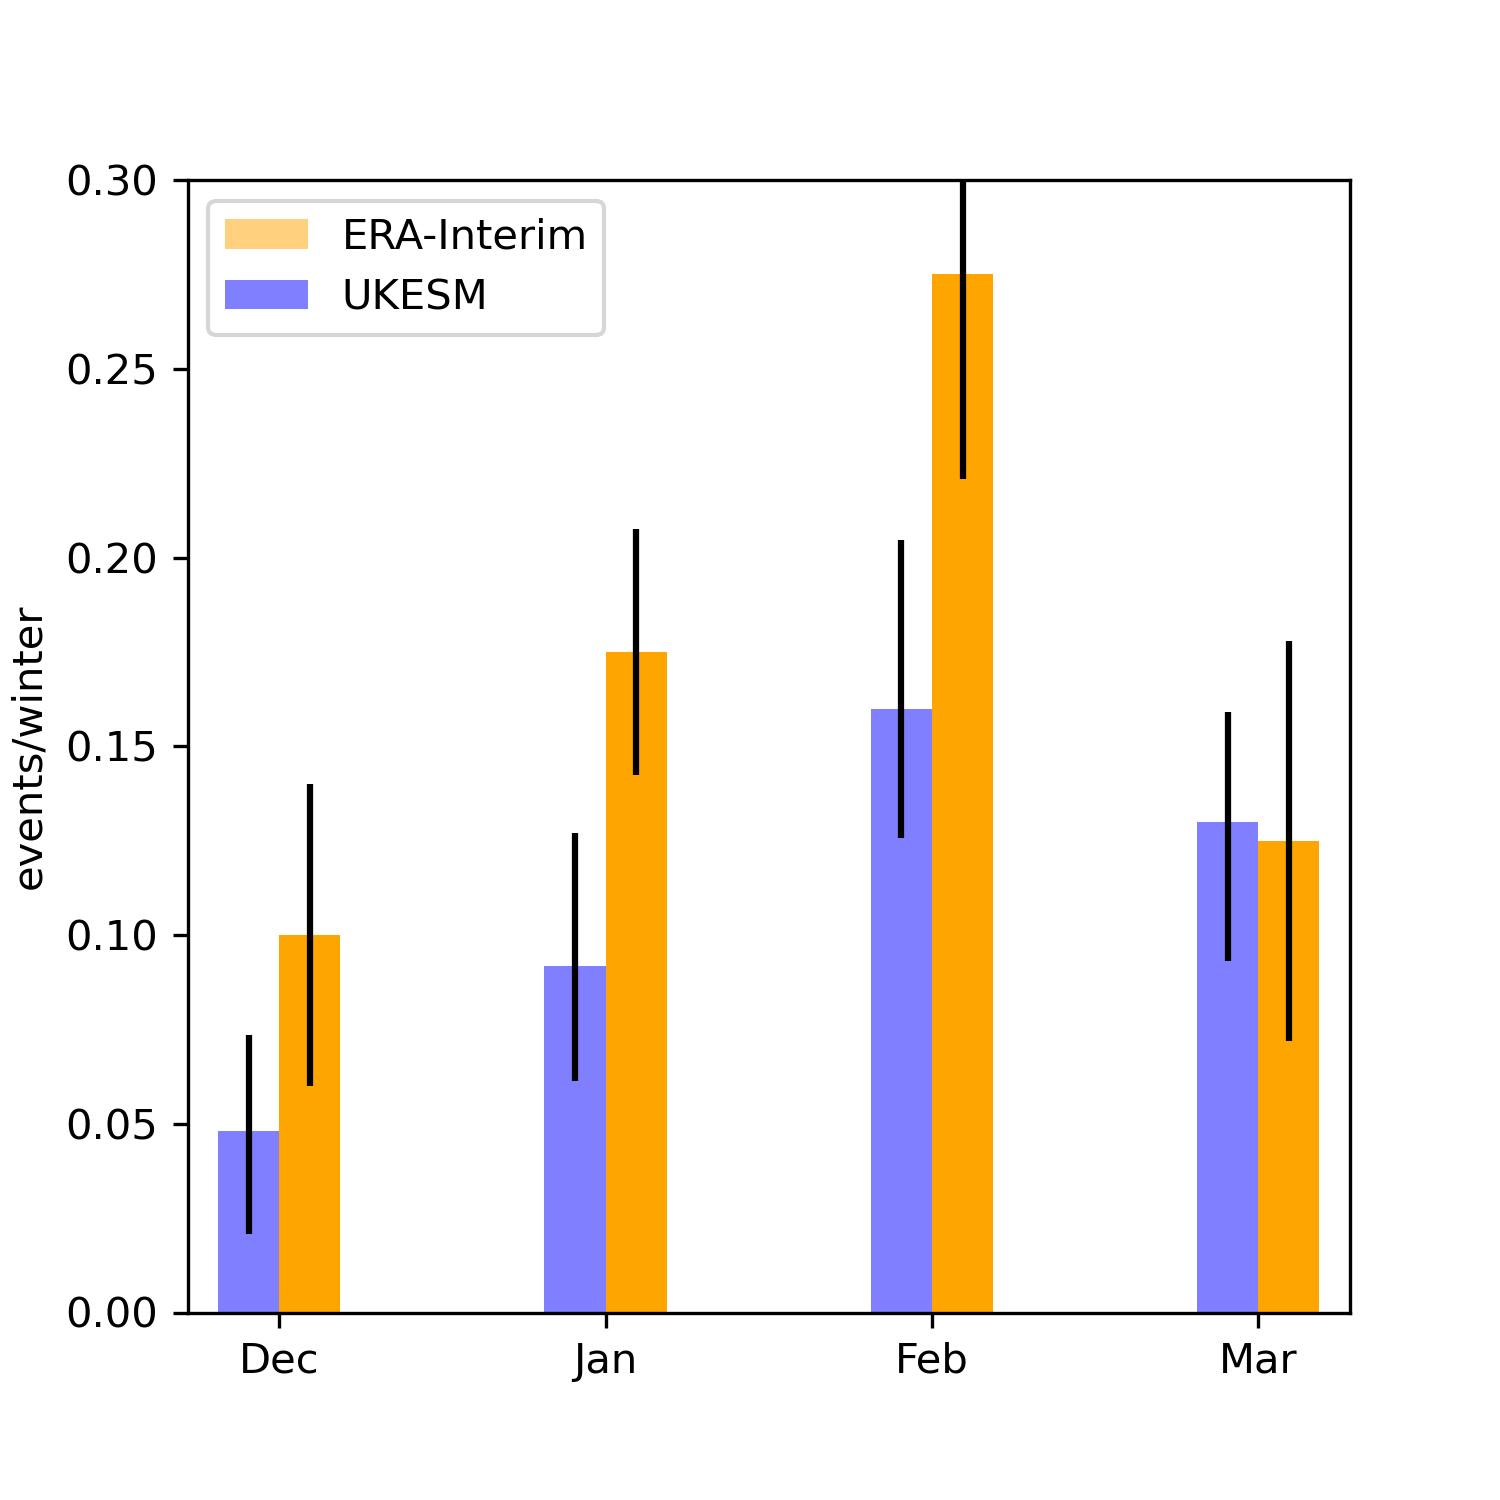
\includegraphics[width = 0.5\linewidth]{figures/SSW_hist_ERA_UKESM.png}
\caption{SSWs per NH winter season separated by month within the UKESM pi-control and ERA-Interim datasets. Error bars are derived using a bootstrap re-sampling method in which random selections of 50 years are chosen from the SSW data and the SSW rate recorded to build a PDF of events per season. 10000 such re-samples are carried out and the 97.5 and 2.5 percentile values are used as error bounds.}
\label{fig1}
\end{figure}
\end{center}

The model exhibits variability in SSW frequency comparable to observations, including both hiatus and consecutive SSW intervals. Figure 2 shows a sample 40-yr interval of the polar vortex zonal wind strength from the UKESM simulation compared with a similar length from the ERA Interim reanalyses. An extended interval of mainly westerly anomalies indicating a strengthened vortex and lack of SSWs can be seen towards the end of the 40-yr interval, similar to the 1990s in ERA-Interim when only 2 SSW events were recorded in the decade. The simulation contains 8 such hiatus intervals with at least 10 consecutive years with no SSWs, the longest of which lasts 16 years. On the other hand, the simulation only contains 2 intervals in which 10 consecutive years exhibit at least 1 SSW. However, if the threshold interval width for identifying hiatus and consecutive-SSW intervals is shortened from 10 to 5 years,  then 9 consecutive-SSW intervals and 25 hiatus intervals are found. These statistics indicate that UKESM is not only able to reproduce the mean state characteristics of SSW events but also decadal-scale variations in SSW rate, underlining its  suitability for this study. 

The second major mode of stratospheric variability is the QBO at equatorial latitudes which is present at all times of the year. Figure 3 shows the equatorial wind time-series from a sample 40-yr interval of the simulation compared with the ERA-Interim dataset. The mean period of the oscillation is longer than observed, at $\sim$38 months compared to $\sim$28 months in ERA-Interim \citep{Kawatani2016}. As a result the vertical shear zones descend less rapidly than observed. There is also a westerly bias at low levels where the QBO-E phase does not extend sufficiently deep into the lower stratosphere, which is a common bias in many models \citep{Bushell2020}. The descending shear zones also appear more regular than observed but there is nevertheless some evidence of decadal-scale variations e.g. in the degree of stalling at 30\ hPa, although not as pronounced as in the observations.

\begin{center}
\begin{figure}[h!]
\noindent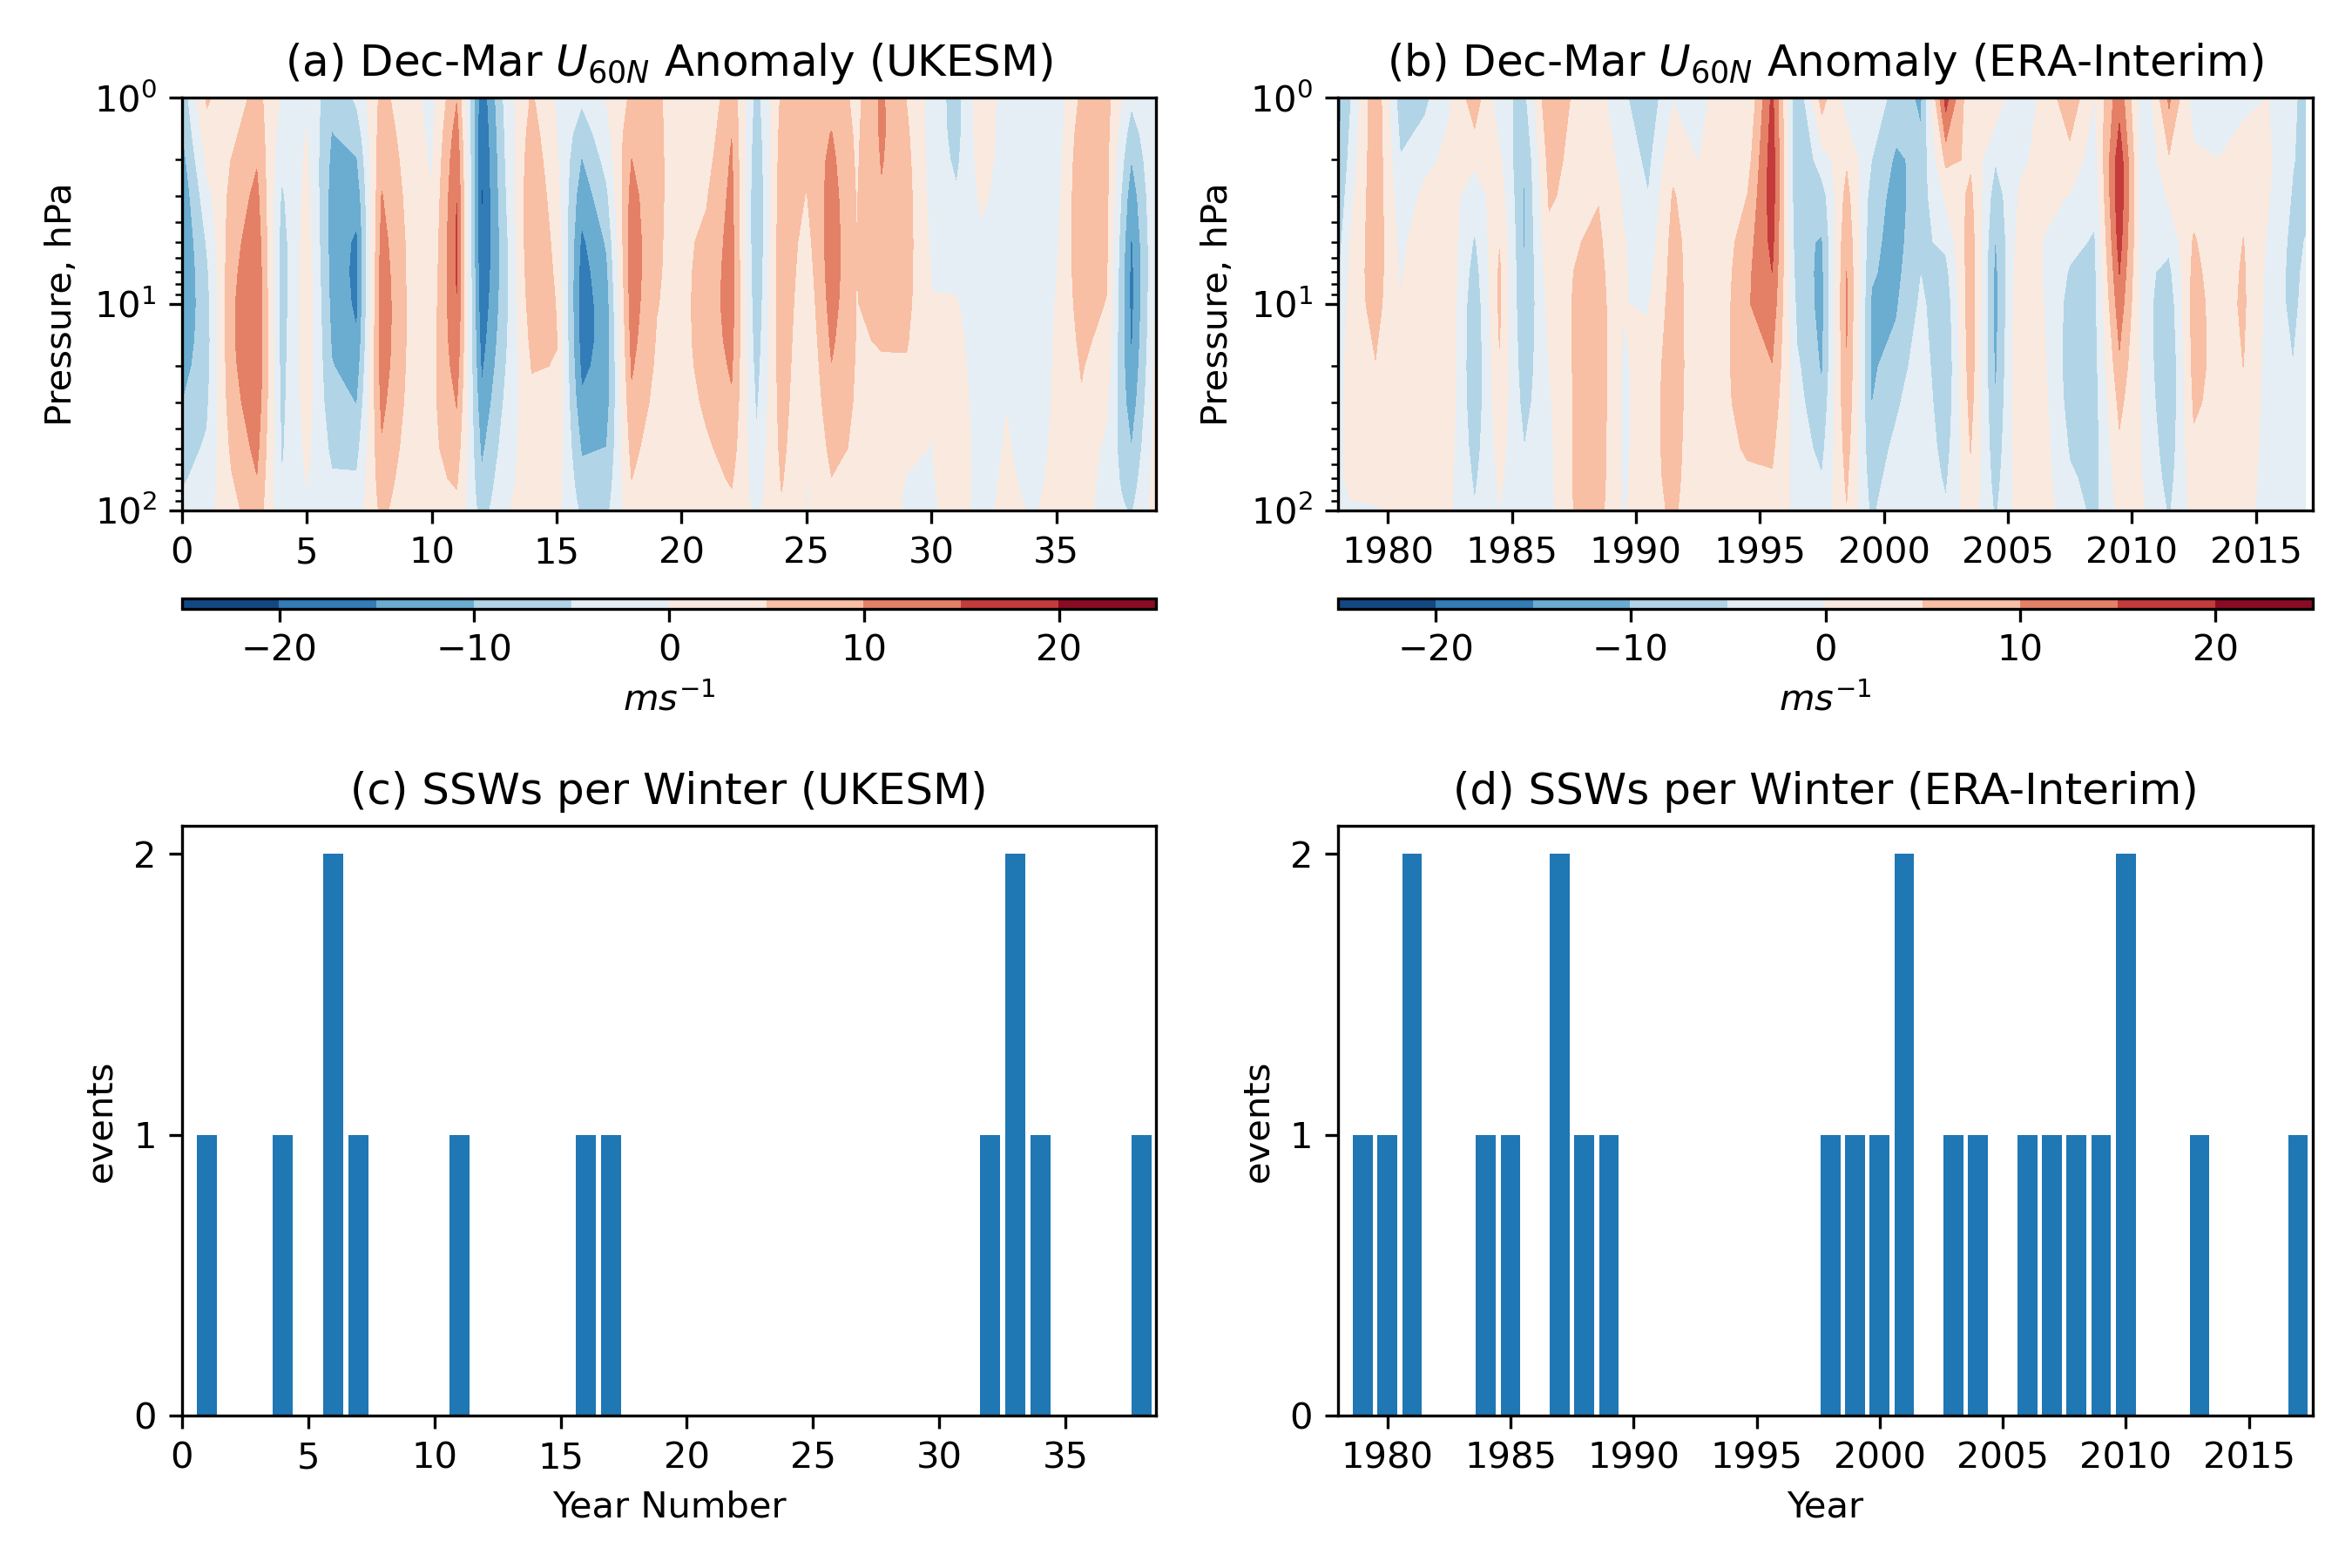
\includegraphics[width = \linewidth]{figures/SSW_series_fig1.png}
\caption{\textbf{(a, b)}: Dec-Mar annual mean ZMZW anomaly from the climatological mean at 60$^\circ$\,N from a 40 year sample from the pre-industrial control simulation of UKESM \textbf{(a)} and the ERA-Interim dataset between 1979 and 2018 \textbf{(b)}. \textbf{(c, d)}: Time series of SSWs recorded per winter season in the same datasets.}
\label{fig1}
\end{figure}
\end{center}

%---------------------------------------------------------------

\begin{center}
\begin{figure}[h!]
\noindent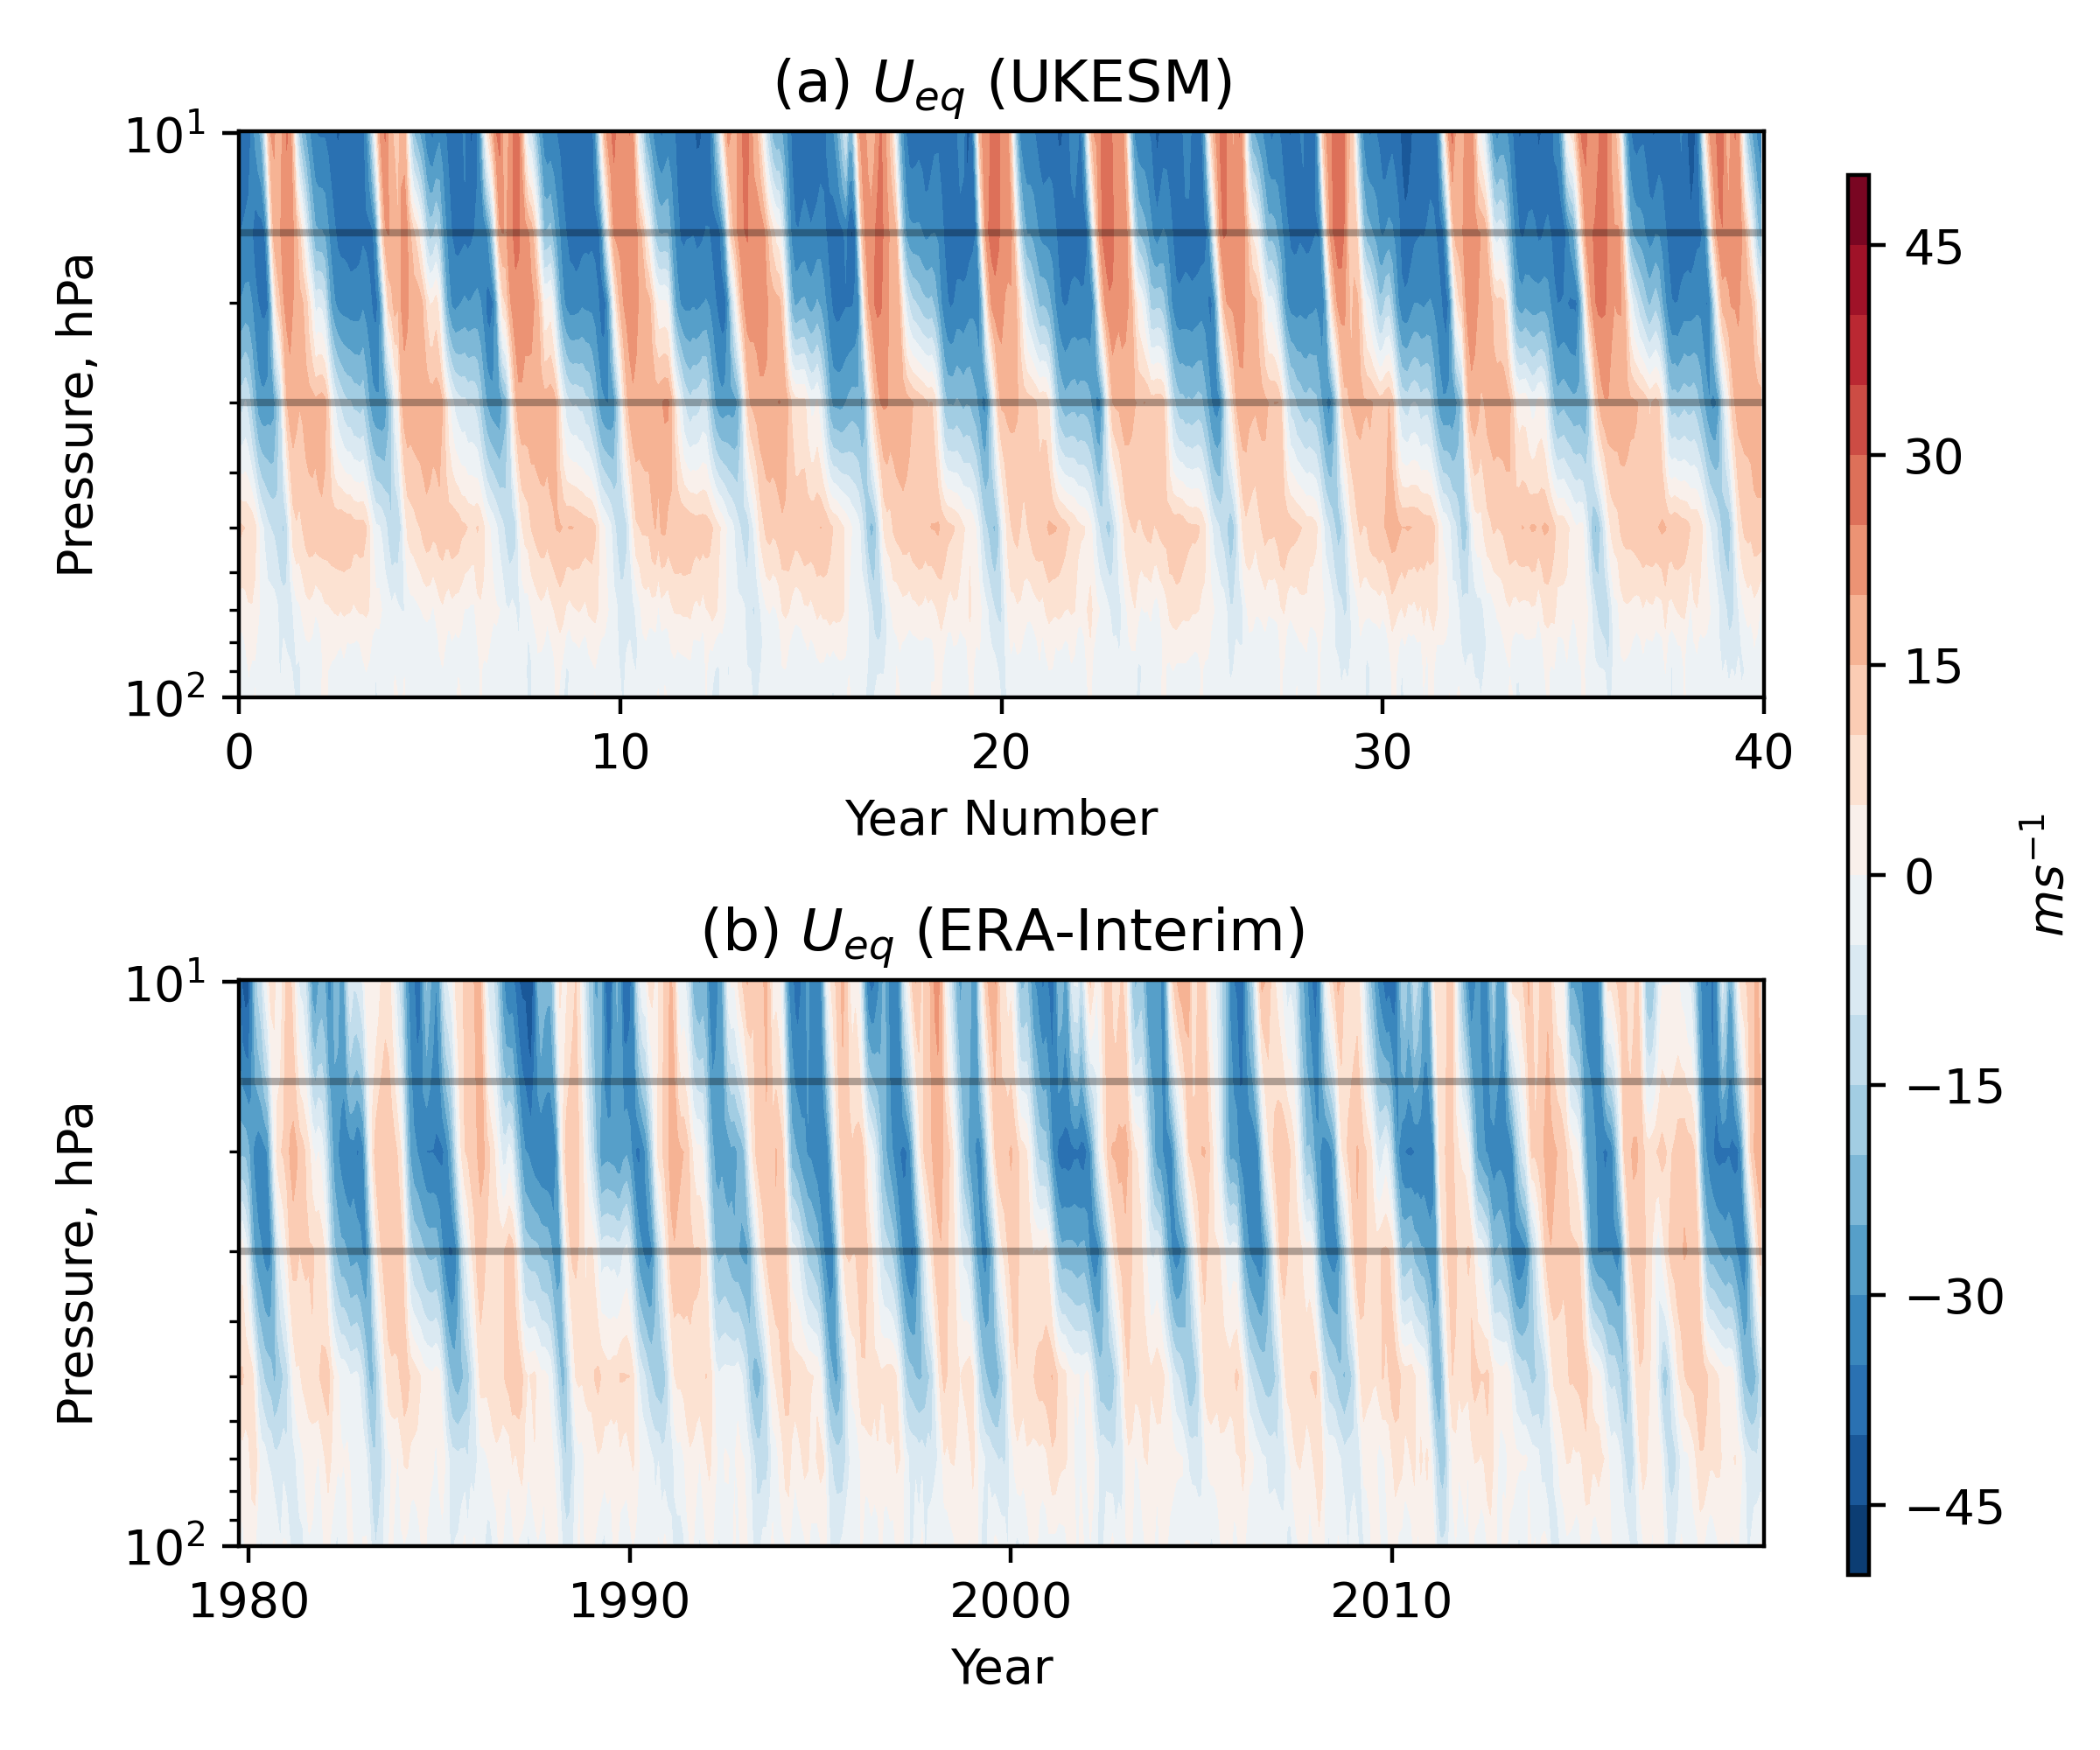
\includegraphics[width = 0.8\linewidth]{figures/QBOs.png}
\caption{ZMZW averaged between 5$^{\circ}$\,S--5$^{\circ}$\,N latitude from from a 40 year sample of the pre-industrial control simulation of UKESM \textbf{(a)} and the ERA-Interim dataset between 1979 and 2018 \textbf{(b)} Horizontal lines mark the 15\,hPa and 30\,hPa levels between which the deep QBO metric employed by \cite{Andrews2019} is defined.}
\label{fig1}
\end{figure}
\end{center}


%---------------------------------------------------------------


There is evidence of coupling between the two major modes of stratospheric variability in the model, giving rise to a Holton-Tan relationship \citep{Anstey20}. Figure 4 shows height-latitude cross-sections of NH winter zonal wind differences between QBO E-W composites defined at various equatorial levels. The familiar pancake structure of alternating easterly / westerly differences is present at equatorial latitudes, indicative of the QBO phase but there is also a response at high latitudes. In good agreement with observations the largest high latitude response amplitude is seen when  the QBO is defined at 50hPa, with anomalously weaker polar vortex strength in QBO-E than in QBO-W years. Higher levels (15\,hPa and 20\,hPa) show little significant QBO-vortex coupling. For comparison we also show in figure 4 the composite different response for QBO composites selected on the basis of the average QBO winds over a greater depth of the equatorial atmosphere (15-30 hPa and 20-50 hPa). We note that while this QBO definition will select some of the same years as in the separate single-level composite definitions, it is specifically designed to identify only QBO  phases that have extended vertical coherence, following \citep{Gray2018} and \cite{Andrews2019}, so the resulting composite  differences in figure 4 will not necessarily be an average of the corresponding single-level differences.   Interestingly, the 15--30 hPa deep-QBO selects years that exhibit not only a weaker polar vortex in QBO-E but also a weaker sub-tropical tropospheric jet (see 200 hPa, 30--40N). This results in a more coherent response in the mid-latitude troposphere and at the surface, in excellent agreement with the results of \cite{Gray2018} and \cite{Andrews2019}. 

%---------------------------------------------------------------

\begin{center}
\begin{figure}[h!]
\noindent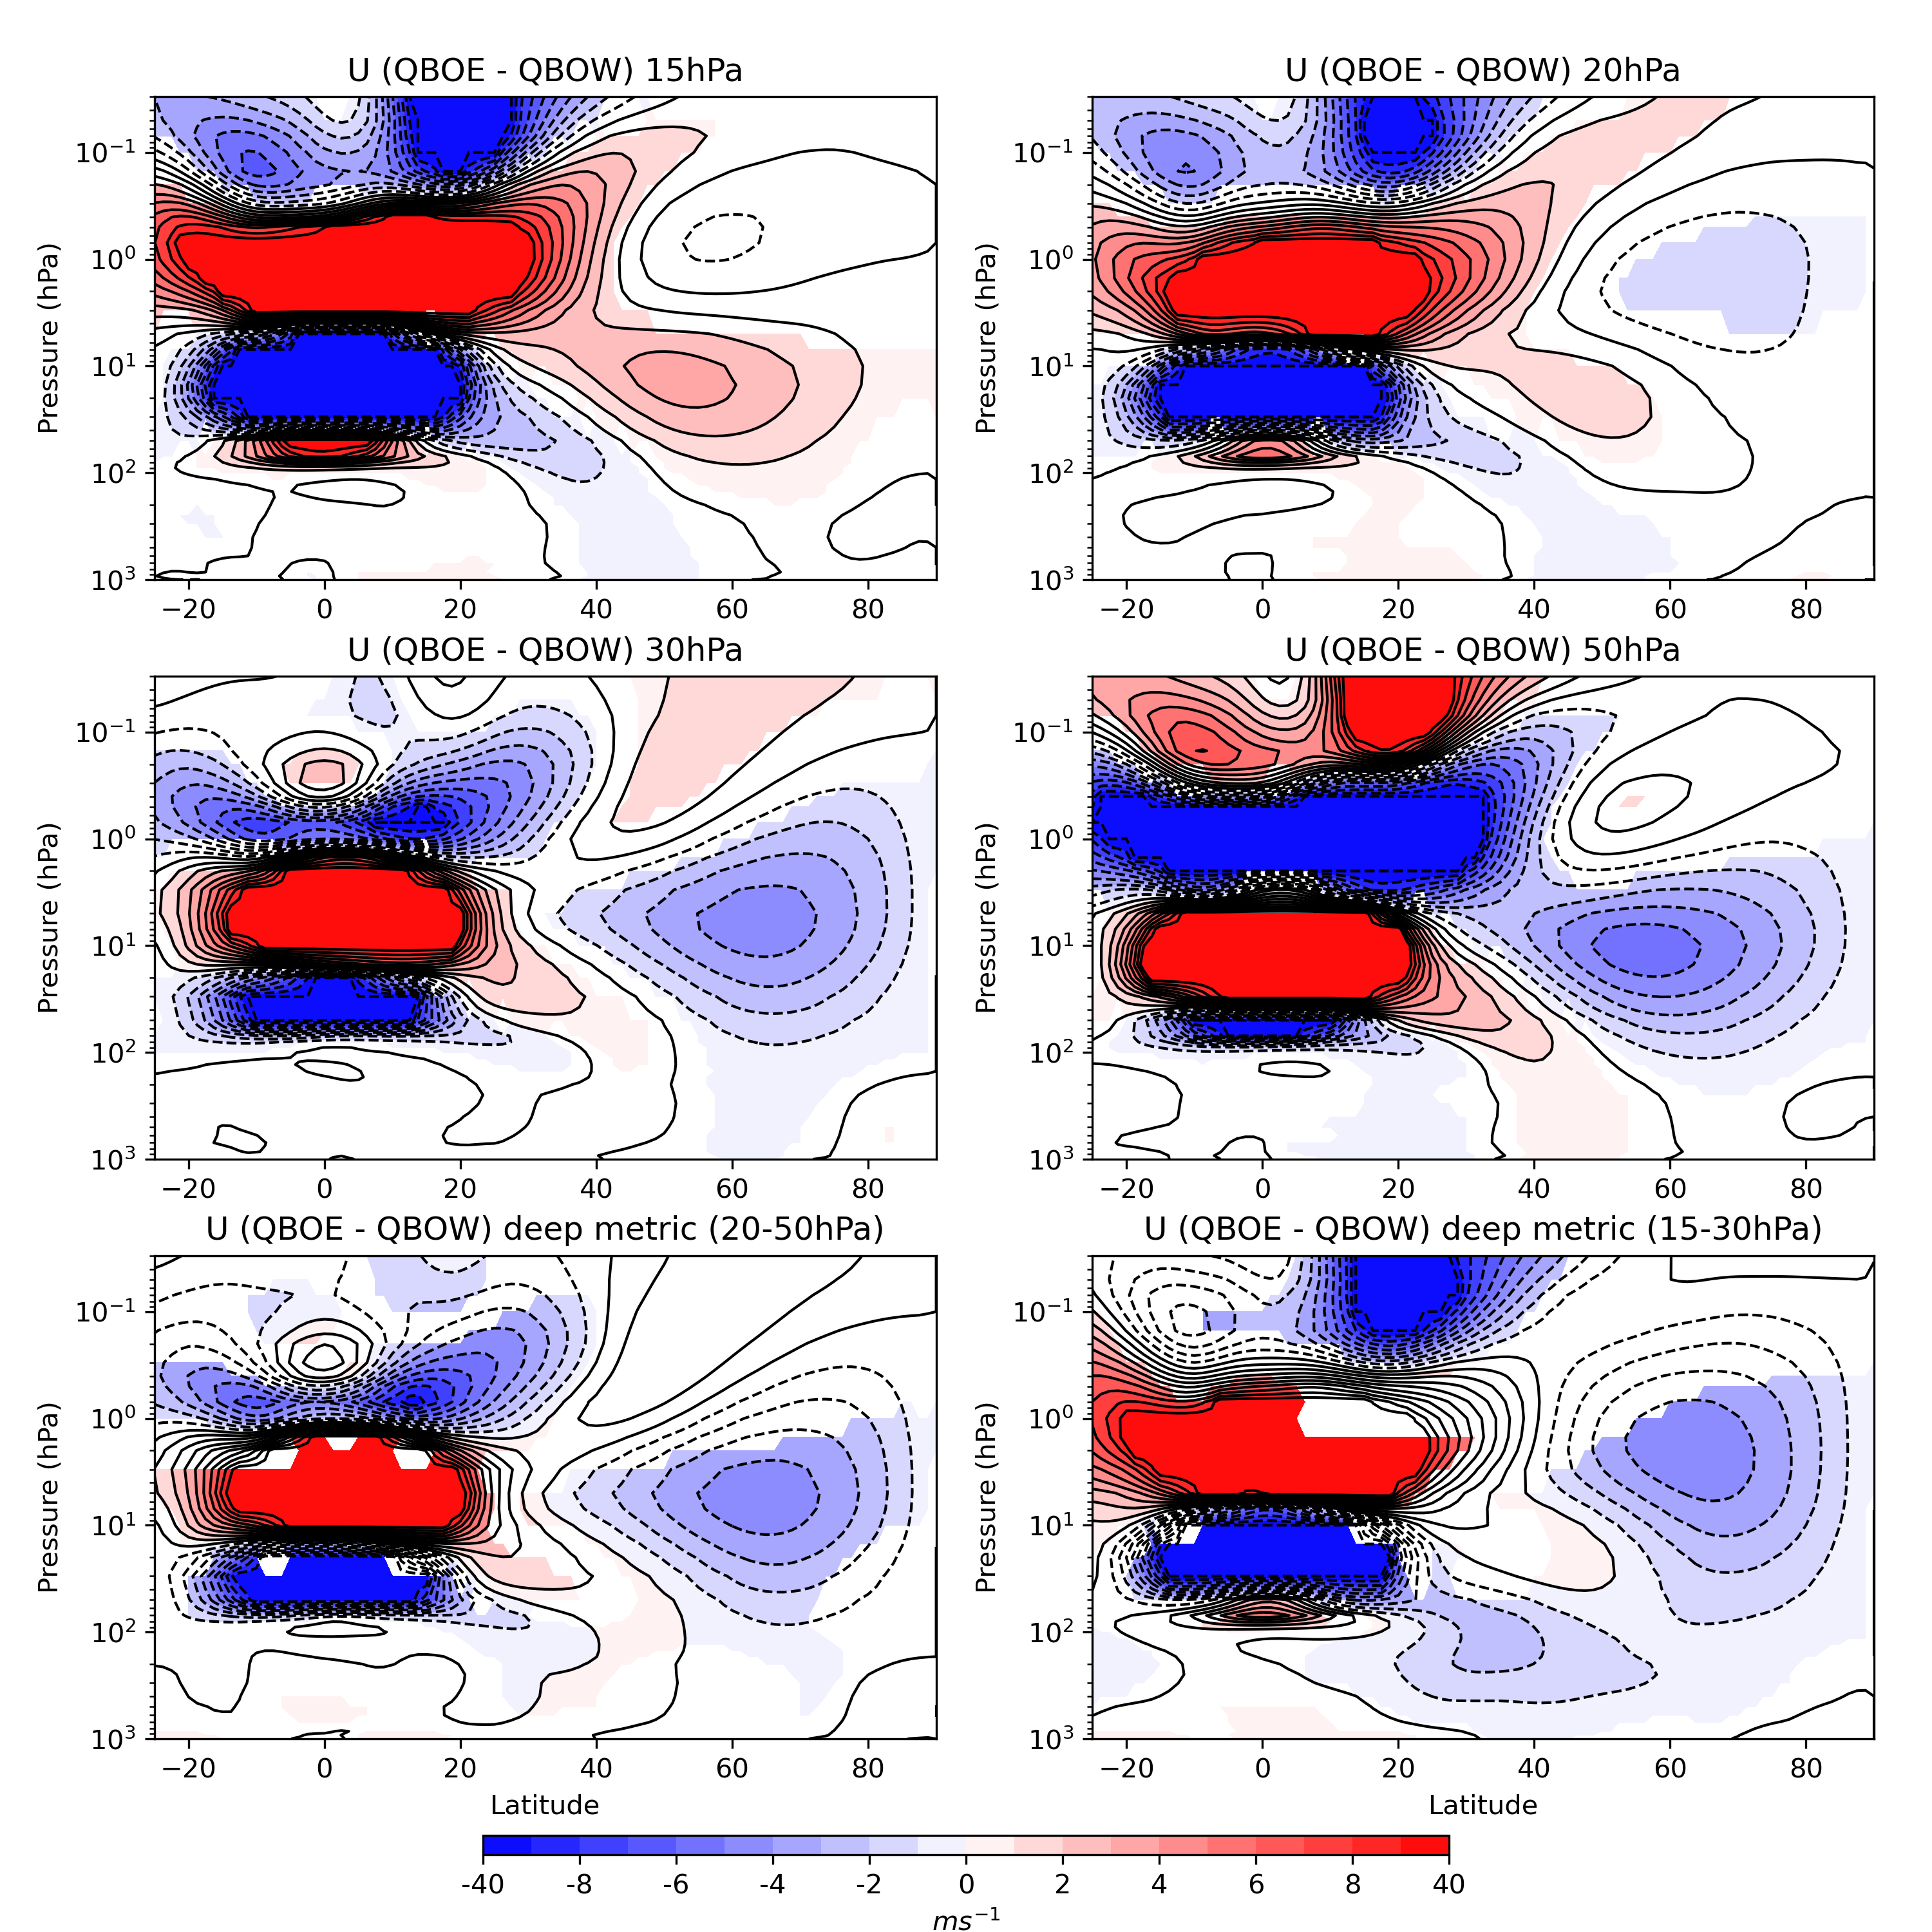
\includegraphics[width = 0.85\linewidth]{figures/Holton_Tan_composite_threshold_fig2.png}
\caption{Dec-Mar ZMZW composite differences between QBO East and QBO West phases evaluated in Sep-Oct at individual levels as well as using the deep QBO metric. The phase of the QBO is defined as in figure 1 - the equatorial Sep-Nov ZMZW of greater magnitude than 5\ m\,s$^{-1}$. Coloured shading indicates differences significant above the 95\% confidence level under a 2 tail student’s t-test.}
\label{fig1}
\end{figure}
\end{center}

The presence of the Holton-Tan relationship is also seen in the modelled frequency of SSWs (figures 5). Significantly higher rates are observed in QBO-E winters than QBO-W. Also notable is the asymmetry in abundance of QBO-E and QBO-W winters - nearly twice as many QBO-E winters are observed compared to QBO-W under all phase definitions (figure 5, legends). This suggests an element of phase locking between the QBO and the seasonal cycle possibly associated with seasonally variations in the strength of mean equatorial upwelling or mid-latitude planetary wave forcing in winter \citep{Pascoe2005, Gruzdez2000, Kylash2015} resulting in QBO phase transitions that occur preferentially in certain months. 

\begin{center}
\begin{figure}[h!]
\noindent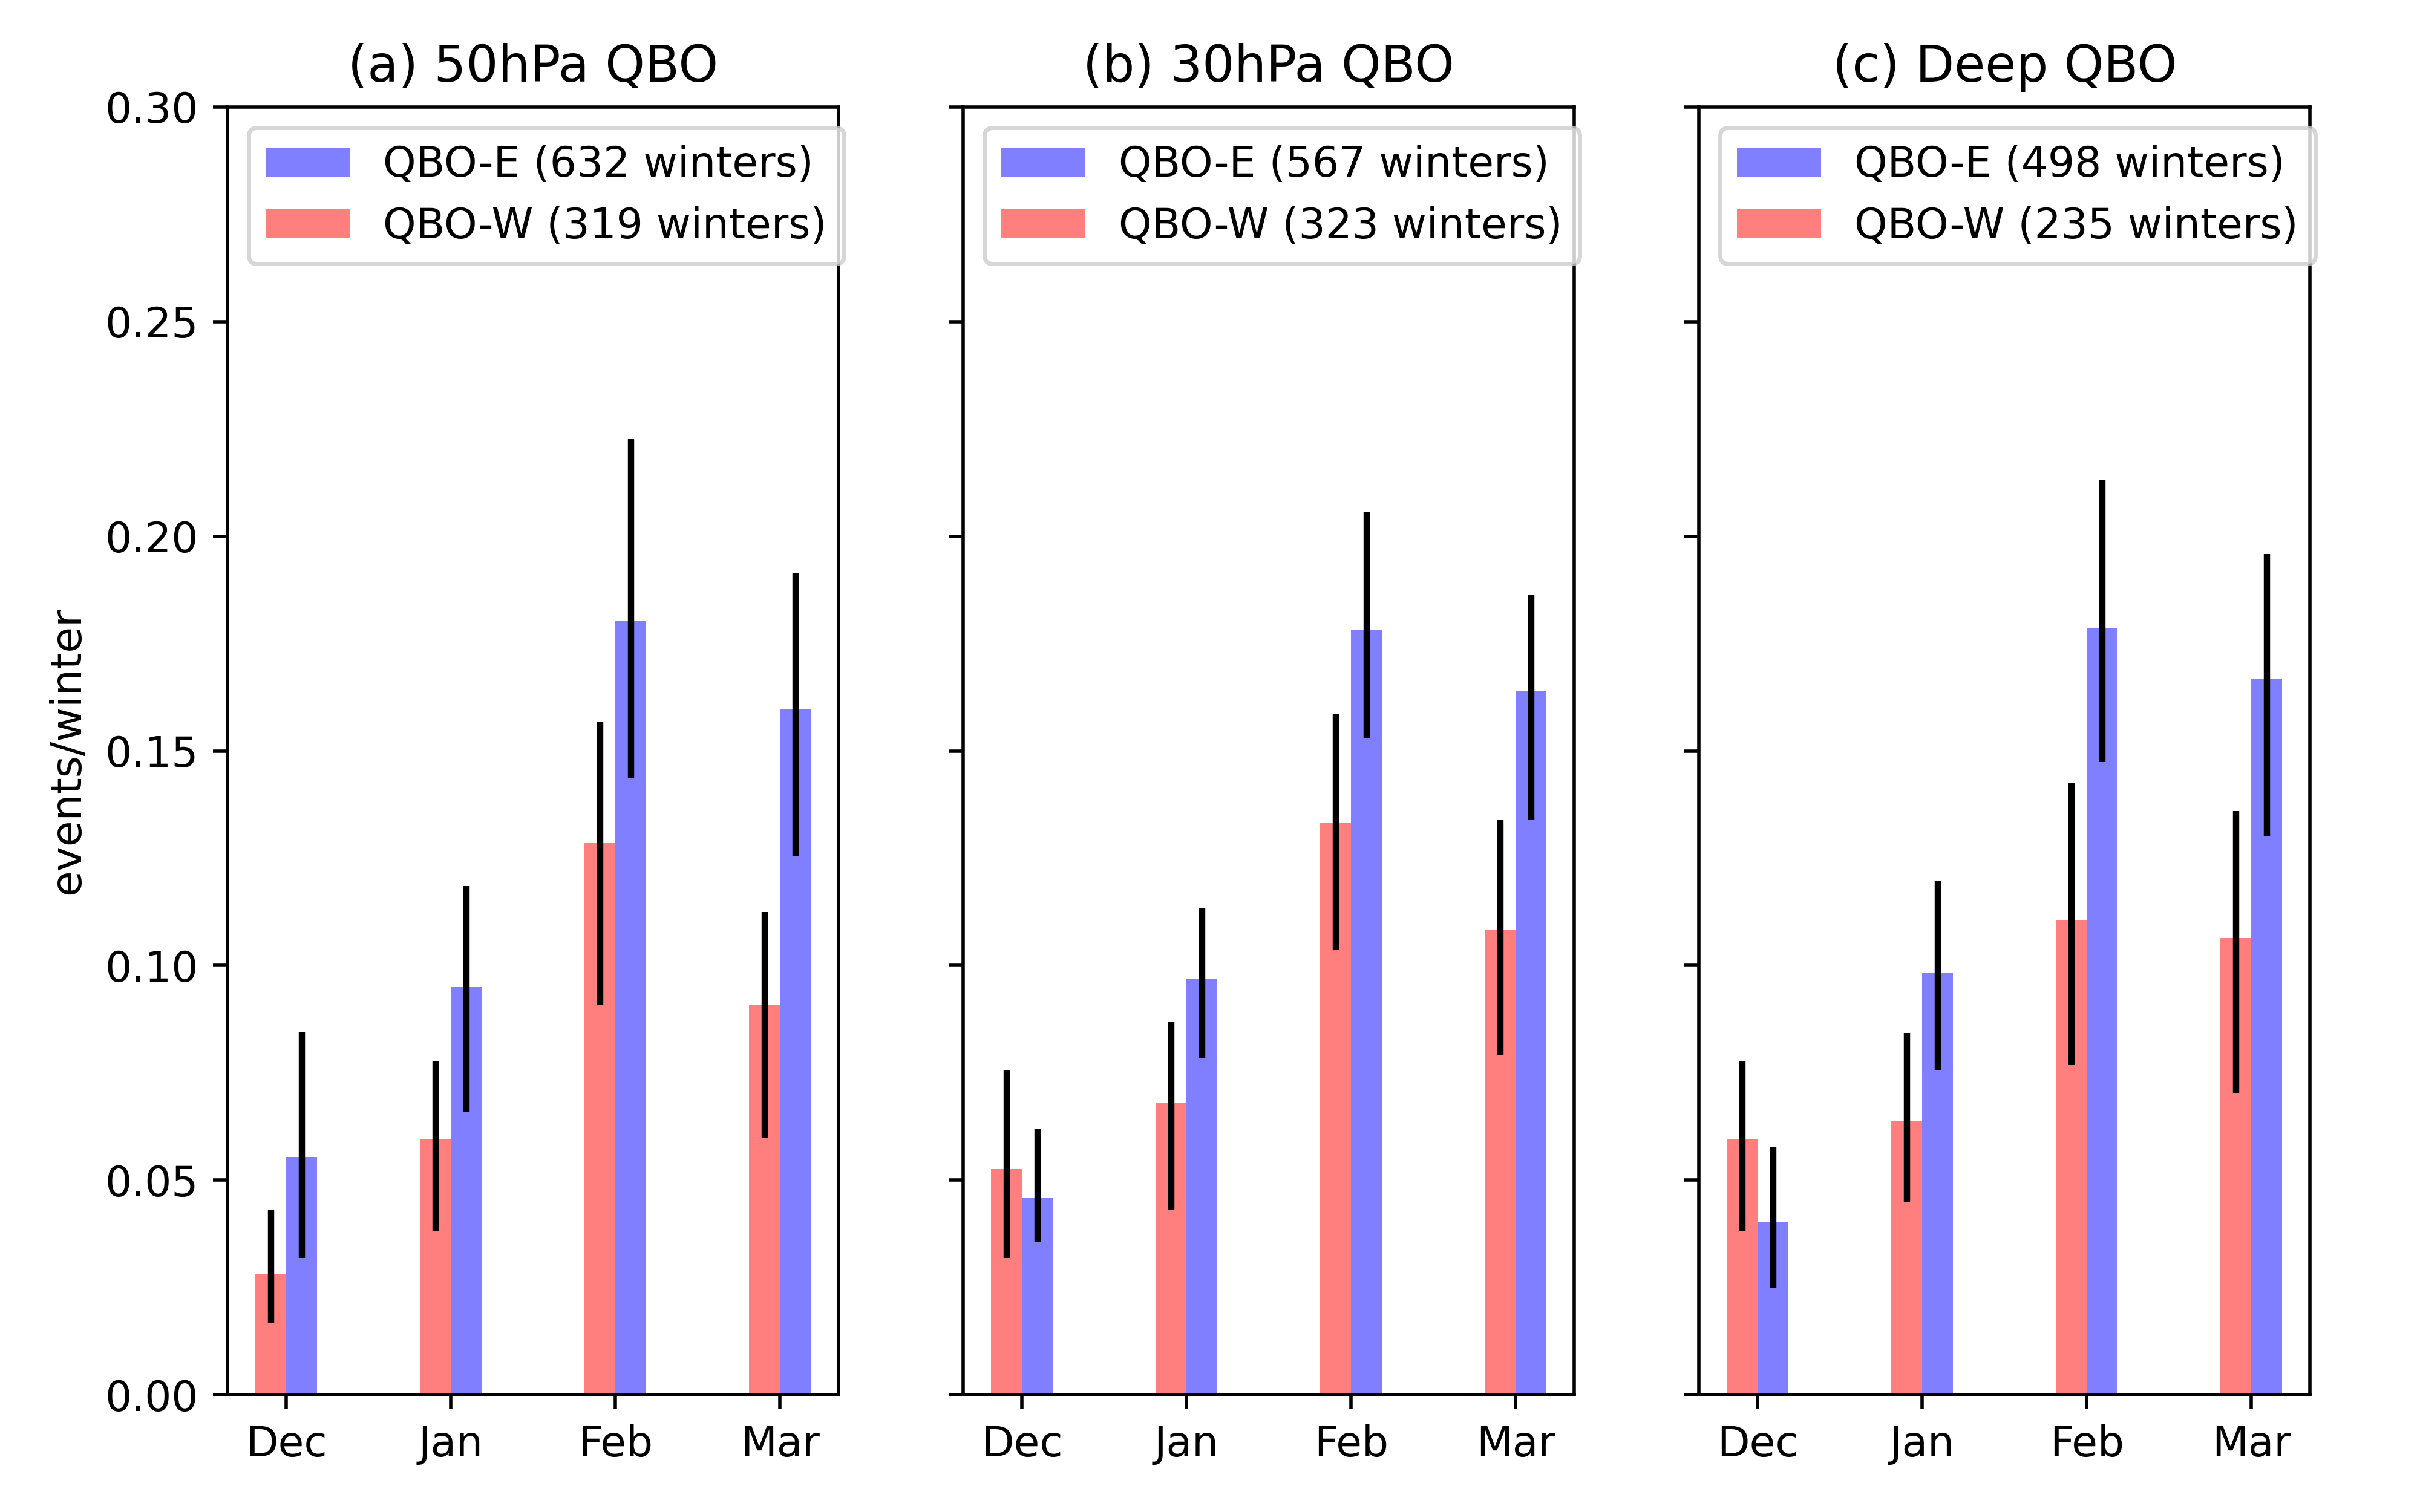
\includegraphics[width = 0.7\linewidth]{figures/SSW_histograms_QBOphases.png}
\caption{SSWs per winter season for years exhibiting QBO-E and QBO-W conditions in early winter (Sep-Nov) defined on different pressure levels (a,b) as well as using the deep metric (c), the vertical mean between 15 and 30\,hPa defined in \cite{Andrews2019}. The QBO phase is defined as any Sep-Nov equatorial ($5^{\circ}$\ S--$5^{\circ}\ $N average) ZMZW that exceeds a magnitude of 5\ m\,s$^{-1}$. Error bars on all plots are derived using the same bootstrapping method outlined in figure 1.}
\label{fig1}
\end{figure}
\end{center}

\subsection{Regression Analysis}
We next employ a multi-linear regression analysis to measure the relative contributions to the time-series of SSWs per year (as in figure 2)  from the QBO, ENSO and the Aleutian low. The results from this analysis are summarised in table 1.  Sensitivity experiments were performed to identify the optimum averaging intervals (lags) for each index: the deep 15-30 hPa QBO index and ENSO3.4 indices  were both defined using early winter (Sep-Nov) averages while the AL index was defined using Dec-Mar averages. The coefficients are all significant to the 95\% level but are relatively small and the $R^2$ score is only 0.047 indicating these variables account for only a small portion of the variability in the SSW timeseries. While results from this multi-linear regression approach are easy to interpret, the approach does not directly tackle the problem posed in this study, that of multi-decadal variability in SSWs and its origins, for two main reasons. Firstly, regression analysis assumes stationarity i.e. it provides a measure of stationary contributions to variability and will only highlight signals that are relatively persistent for the whole simulation. Secondly, it  analyses variability in the time series at all timescales simultaneously, so that the results are dominated by the timescales with larger amplitude variations.  This means that the results in table 1 are most likely dominated by the shorter (inter-annual) timescales and any small amplitude variations at longer timescales will not be revealed. The latter can be addressed to some extent by smoothing or filtering the time-series, as discussed in the next section, but this requires prior knowledge of which frequencies are of interest. An alternative and superior approach to this problem employs wavelet analysis, described more fully in the next section, which successively examines the frequency intervals to identify the presence of signals thus avoiding dominance by one particular frequency, and also examines the time evolution of the signal so that non-stationary signals can also be identified. 

\begin{table}[h!]
\centering
\begin{tabular}{|p{3cm}||p{3cm}|p{3cm}|}
 \hline
 \multicolumn{3}{|c|}{SSW regression}\\
 \hline
 Regression Variable& Coefficient& p value\\
 \hline
 ENSO3.4  & 0.1625$^+_-$0.035& 0.0002\\
 AL  &   -0.0927$^+_-$0.04  & 0.048\\
 deep QBO  & -0.1993$^+_-$0.03&0.0001\\
 \hline
 \end{tabular}
\begin{center}
\caption{Summary of results from regression analysis of SSWs per NH winter time series.}
\end{center}
\end{table}

%---------------------------------------------------------------

\subsection{Long-term Variability of the Polar Vortex}
A more comprehensive assessment of the long-term variability of SSWs can be made using a wavelet power spectrum approach. We count the number of SSWs in each winter season (Dec-Mar) and calculate the corresponding wavelet power spectrum, shown in figure 6. As described above, the analysis highlights the presence of power in the signal as a function of frequency (period in years, along the y-axis) and as a function of time (year of simulation along the x-axis). As expected, there is an intermittent but relatively persistent signal with period around 2-4 years throughout the simulation, corresponding to the period of the QBO which supports the presence of a Holton-Tan relationship between the QBO and the polar vortex in the model. The so-called 'global power spectrum' (i.e. the time average of the wavelet spectrum) shown on the right of the figure shows that the signal is on the boundary of the 95\% statistical significance. Other signals at periods near 20-30 years are similarly intermittent and manifest as a peak in the time-averaged spectrum that is also near the 95\% significance boundary. The most persistent feature of the series appears at periods between $\sim$60-90 years in the interval between 400-800 yrs. This feature shows statistical significance (based on comparisons between power in the spectrum and that of an AR1 process with the same autocorrelation structure as the series being analysed) for around 350 years of the 1000-yr simulation but does not cross the significance threshold for the time-averaged spectra. There is a possible limitation of this wavelet methodology due to the discrete nature of the time series being analysed (time points take values 0/1/2). The Morlet wavelet is a continuous function and, as a result, convolution with a highly discretised series may alias features on the resulting wavelet spectra. This limitation must be considered when drawing conclusions from the wavelet spectra and is discussed further below.

\begin{center}
\begin{figure}[h!]
\noindent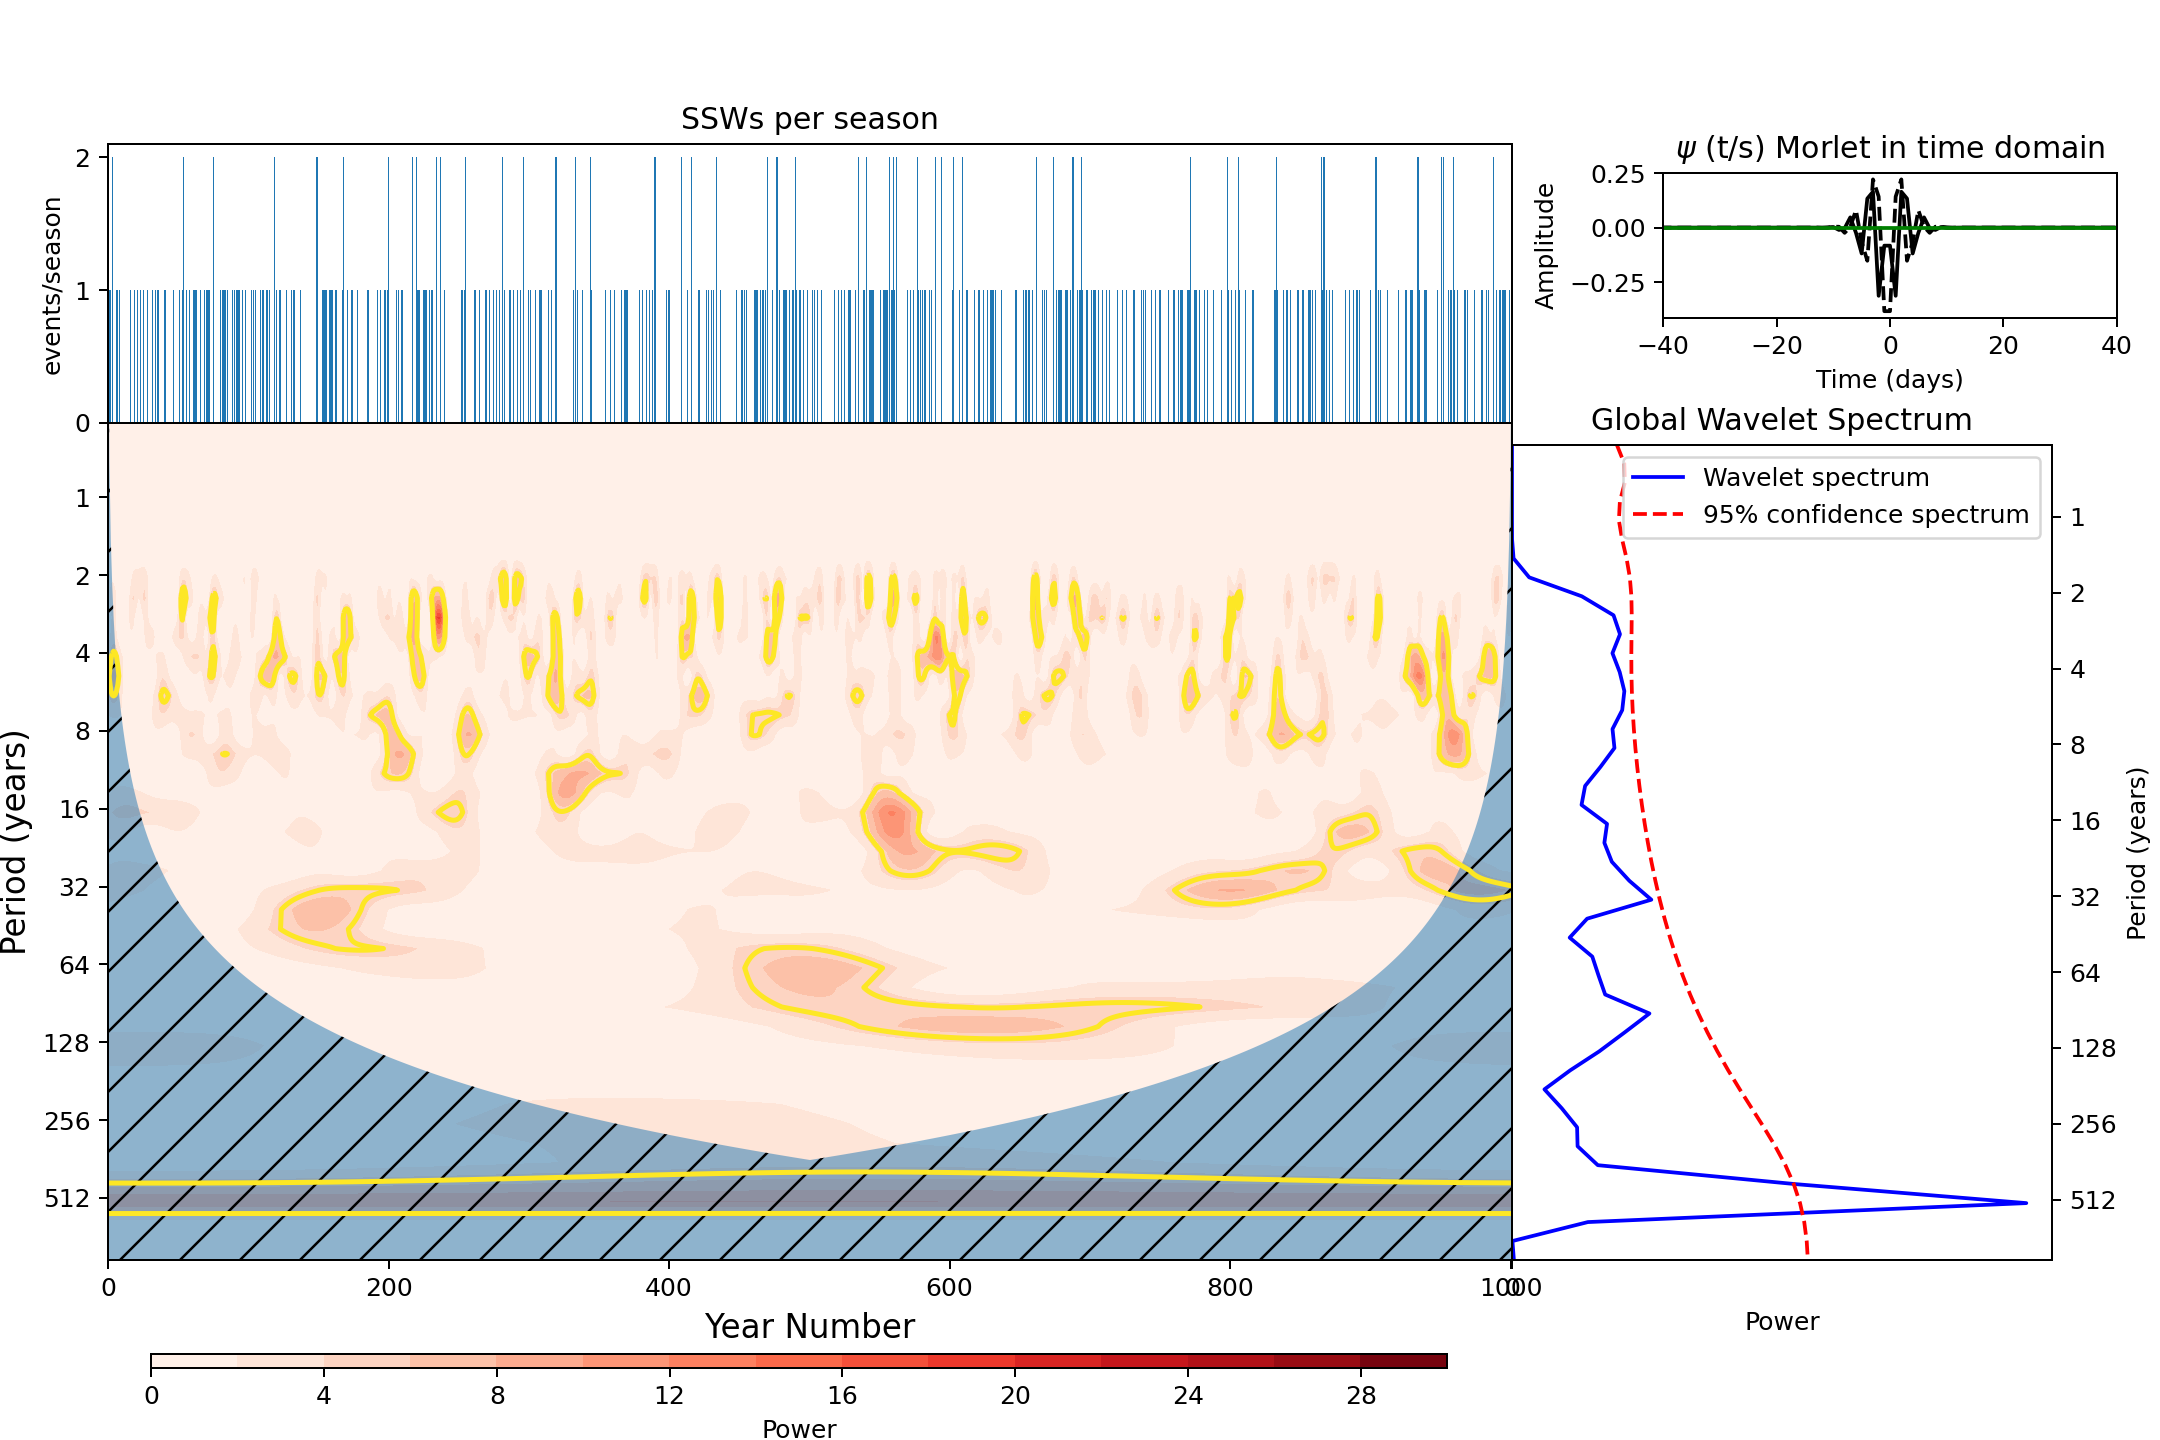
\includegraphics[width = 0.8\linewidth]{new_changed_figures/SSW_wavelet_new_levels.png}
\caption{\textbf{Top left}: SSW events per Dec-Mar season in UKESM \textbf{Bottom left}: Wavelet power spectrum of time series in top left. Hatching represents area outside the cone of influence in which edge effects are significant and power should not be considered. Yellow contours represent the 95\% confidence level assuming mean background AR1 red noise. \textbf{Top Right}: Morlet wavelet used for the wavelet transform in the time domain. \textbf{Bottom right:} Global power spectrum, the wavelet power averaged over the whole simulation (blue line), and global 95\% confidence spectrum (red dashed line).}
\label{fig3}
\end{figure}
\end{center}

%---------------------------------------------------------------

The focus of this study is on the longer-term time variations to understand the source of variability characterised by hiatus intervals (no SSWs over an extended period) and consecutive-event intervals (at least one SSW every year for an extended period). We therefore apply low-pass filtering to the time series of SSWs per season using a 5-year rolling window and examine the spectral characteristics of this smoothed series (which we refer to henceforth as $SSW_{5yr}$). This averaging is similar to the standard practice of smoothing daily data to remove the noise associated with daily weather variations, thus isolating longer seasonal timescales. It also decreases the impact of the time series discretisation by reducing the chance of introducing spurious spectral features on the wavelet power spectrum which could be otherwise encountered when analysing the un-smoothed time series.  

\begin{center}
\begin{figure}[h!]
\noindent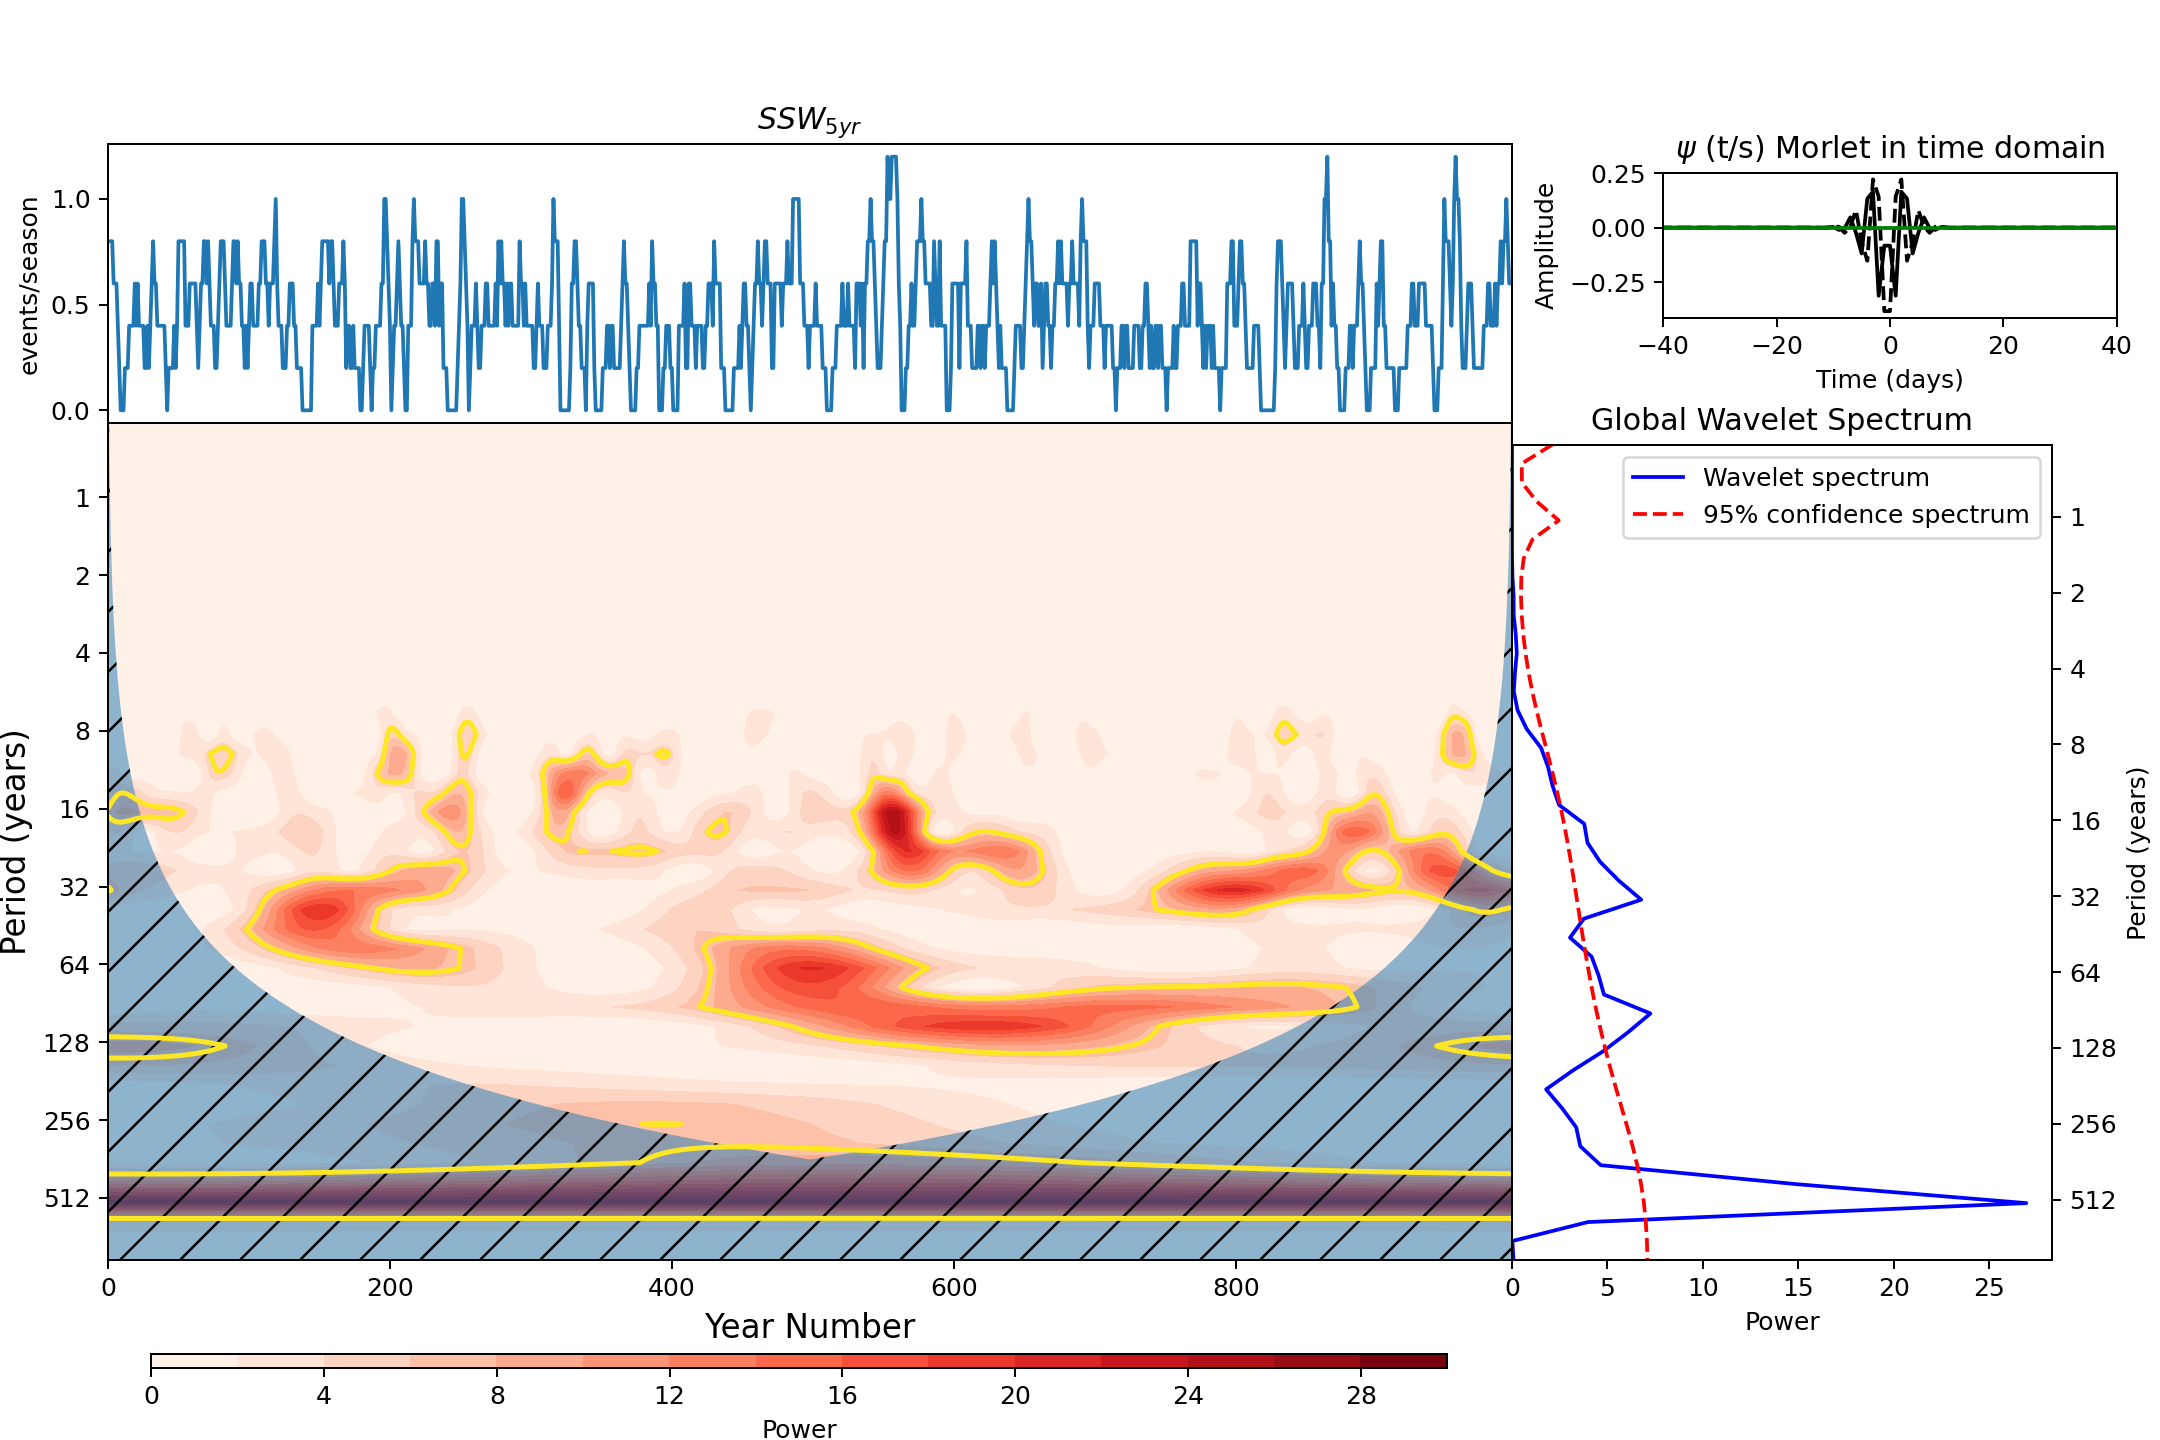
\includegraphics[width = 0.8\linewidth]{new_changed_figures/SSW_wavelet_5_yr_fig3_new_levels.png}
\caption{\textbf{Top left}: SSW events per Dec-Mar season in UKESM smoothed using a 5 year running mean. \textbf{Bottom left}: Wavelet power spectrum of time series in top left. Hatching represents area outside the cone of influence in which edge effects are significant and power should not be considered. Yellow contours represent 95\% confidence level assuming mean background AR1 red noise. \textbf{Top Right}: Morlet wavelet used for the wavelet transform in the time domain. \textbf{Bottom right:} Global power spectrum, the wavelet power averaged over the whole simulation, and global 95\% confidence spectrum.}
\label{fig3}
\end{figure}
\end{center}

%---------------------------------------------------------------
The wavelet power spectrum of $SSW_{5yr}$ (figure 7) shares many of the characteristics of the spectra of the un-smoothed series (figure 6), but the longer period signals are now more clearly evident, as expected. The $SSW_{5yr}$ wavelet spectrum shows the two broad regions of statistically significant maxima corresponding to signal periods of $\sim$20-30 years and $\sim$60-90 years, but with increased significance both locally and in the time-average. For example, the feature around 90 year period appears significant for 450 years in $SSW_{5yr}$ compared to 350 years before smoothing. One possible explanation for this increase lies in our definition of the significance level on power which is dependent on the lag-1 autocorrelation of the time-series. Introducing a 5 year averaging window will increase the autocorrelation, possibly leading to a less strict significance level. However, this is unlikely because the significance level is constructed using a red noise process with the same autocorrelation as the series. This means that for $SSW_{5yr}$, the threshold for 95\% confidence level increases with increasing period more steeply than in the un-smoothed case and yet the power exhibited at those long periods in $SSW_{5yr}$ nevertheless achieves higher statistical significance. This indicates that the smoothing has enhanced the visibility of a real signal in the $SSW_{5yr}$ time series that was less visible in the un-smoothed time-series. As a check for robustness, we also include the $SSW_{5yr}$ wavelet spectrum including November SSW events (supp figure A1). it looks similar to  the spectrum shown in figure 7 particularly on $\sim$60-90 years timescales with persistent power for around 450 years of the simulation at these periods.  


\subsection{Surface Forcing of Polar Vortex Variability}
In the absence of external forcing mechanisms such as greenhouse gas or anthropogenic aerosol forcing, the presence of long-term variability such as the 60-90 year periodicity seen in $SSW_{5yr}$ (figure 7) suggests a source of long-term internal variability from within the climate system. 

The most obvious potential driver of such long timescale variability is the ocean due to its high degree of thermal inertia. Previous work has identified coupling between tropical SSTs and the polar vortex, such as the relationship to ENSO conditions (see section 1). The model exhibits an expected connection between ENSO and the vortex on interannual timescales indicated by the regression analysis results (table 1) and ZMZW composites for El Ni\~{n}o and La Ni\~{n}a winters (supp figure A2). Figure 8a shows the wavelet power spectrum for the 5 year smoothed Sep-Nov ENSO 3.4 index as well as the cross power spectrum with $SSW_{5yr}$. We use the early NH winter ENSO index to capture the lagged response of the vortex to this mode of variability. The ENSO index is slowly varying so will likely remain in the same state between early and mid-winter. We also smooth the ENSO index for the purposes of calculating the cross spectrum with $SSW_{5yr}$. (The spectrum of the un-smoothed ENSO 3.4 index is provided in supp figure A3 and shows significant power in the expected period range of 4-7 years \citep{Santoso2017}). The smoothed ENSO 3.4 index shows intermittent power at periods around 16 years which appears significant in the global spectrum. It also exhibits a small signal coincident with the 90 year variability in $SSW_{5yr}$, however this feature only persists for around 100 years of the simulation. Cross spectra between the two series (figure 8b) reveals that the coincidence in signals at the 90 year period, while significant under our test, is marginally prominent but only covers a small proportion of significant signals in $SSW_{5yr}$. This suggests there may be some contribution from ENSO to the observed SSW variability but it is only marginally significant and on its own it cannot explain the signal in $SSW_{5yr}$ that persists for 450 years. The source of this ENSO signal at 90 year periods is unclear, although the PDO spectrum shares some of the same characteristics on the 90 year timescale (supp figure A4) which is consistent with results of \cite{Newman2016} which proposes the PDO as a low pass filtered version of ENSO. 

\begin{center}
\begin{figure}[h!]
\noindent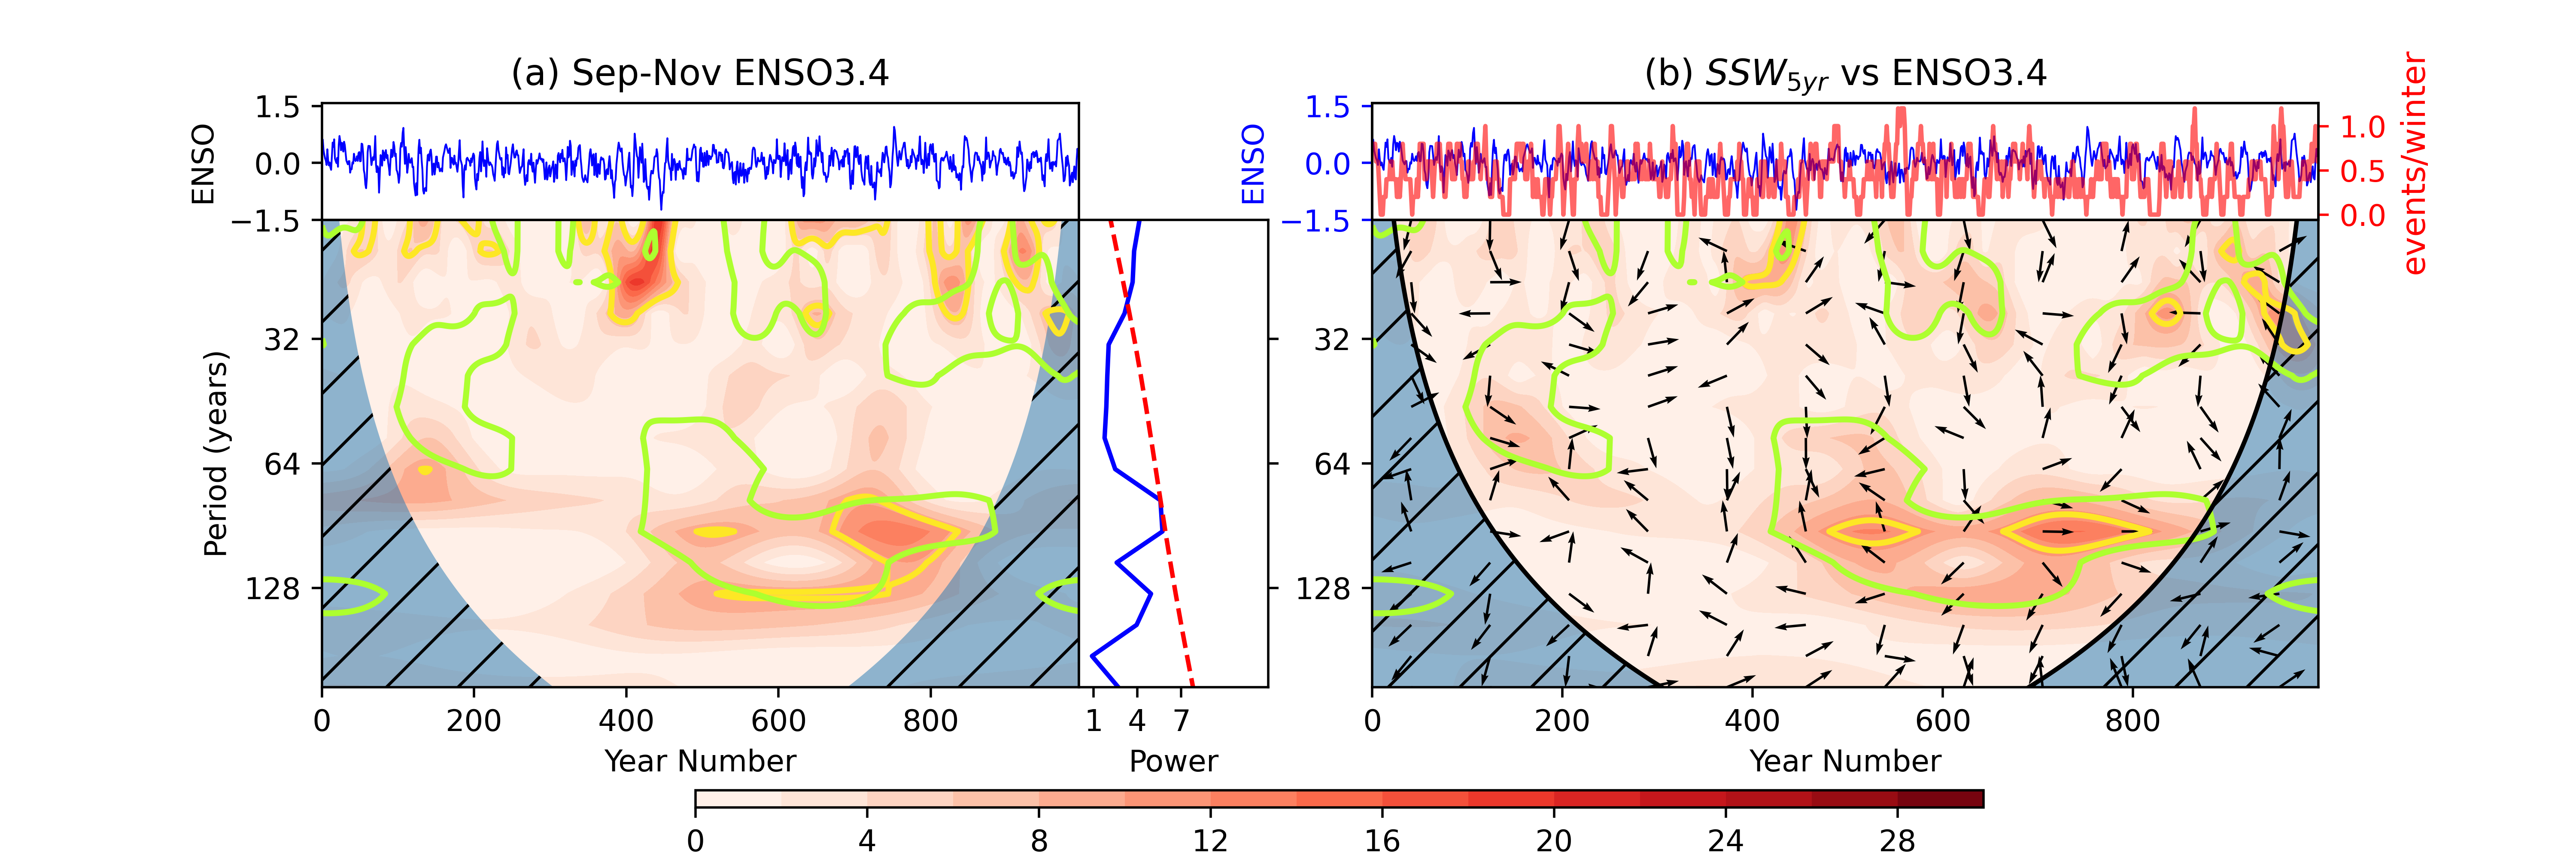
\includegraphics[width = \linewidth]{new_changed_figures/ENSO_wavelet_combined_new_levels.png}
\caption{\textbf{(a, top)}: ENSO3.4 time series, \textbf{a, bottom left}: Wavelet power spectrum (shaded contours represent wavelet power and yellow contours the 95\% significance level compared to an AR1 process), \textbf{a, bottom right}: global wavelet power spectrum (blue) and 95\% confidence level (dashed red). \textbf{b}: Cross spectra between $SSW_5yr$ and the ENSO3.4 index. \textbf{b, top}: ENSO3.4 and $SSW_5yr$ time series. \textbf{b, bottom}: Cross power spectrum. Shading indicates cross power, yellow contours the 95\% confidence interval and arrows the relative phase angle between signals in the time series (to the right: in phase, vertically upwards: $\frac{\pi}{2}$ out of phase with SSWs leading, to the left: $\pi$ out of phase, vertically downwards: $\frac{\pi}{2}$ out of phase ENSO3.4 leading). Green contours on both spectra represent the 95\% confidence intervals for the wavelet power spectrum of $SSW_{5yr}$.}
\end{figure}
\end{center}

In the interest of completeness, we also explore the long-term variability of other tropical ocean regions and their potential teleconnections with the polar vortex. Four additional tropical regions were selected based on those identified by \cite{Scaife2016} and outlined in section 2. While all four regions show some elements of multi-decadal variability (supp figure A5), particularly the Tropical Atlantic with a peak period of approximately 140 years for 700 years of the simulation, none of the spectra show variability that coincides well with that of $SSW_{5yr}$. There is some overlap of the Atlantic and Tropical East Pacific spectra with the regions of significant periodicity at around 60-90 years in the $SSW_{5yr}$ spectrum but, like the ENSO3.4 index, the overlaps and cross power between the series (supp figures A3 and A4) are minimal and cannot reasonably explain the vortex signal, especially the signal of period approximately 90 years that persists in $SSW_{5yr}$ for around 450 years (supp figures A3 and A4, green contours).

The strength of the Aleutian Low (AL) has also been used as an indicator of tropospheric wave forcing and its influence on the polar vortex \citep{Woo2015}. A similar wavelet and cross-spectrum analysis was therefore performed using an index based on the strength of the modelled NH winter (Dec-Mar) AL (see section 2 for details). The wavelet power spectrum for the 5-year smoothed AL index (figure 9a) exhibits elements of periodic signals with maximum power corresponding to a period of around 55 years (between 40-60 years) but with fairly minimal overlap with the regions enclosed by the 95\% confidence level in the corresponding SSW wavelet analysis (green contours). AL indices derived from different winter months give similar spectral patterns (not shown).  The cross spectrum analysis between the AL and $SSW_5yr$ (figure 9b) highlights this relatively small region of overlap in the interval between years 400-500. However, the phase relationship, indicated by the arrows in that region of overlap is difficult to interpret. The proposed physical mechanism of coupling between the AL and the vortex \citep{Woo2015} involves an association between a deeper AL (i.e. lower pressure and hence a negative anomaly) with increased frequency of SSWs. This negative correlation would give rise to arrows pointing to the left if the relationship was present. In contrast, the upward arrows in figure 9b indicate a $\frac{\pi}{2}$ phase difference between the indices on these 60 year timescales, suggesting that peaks in $SSW_{5yr}$ variations are associated with maximum rates of change of the AL index at the same periods. As with ENSO3.4, the spectra of the AL shares some features with that of the PDO (supp figure A4). This is consistent with studies into these modes of variability which find significant correlation of the PDO and AL \citep{Mantua_1997, Rodionov2005} as well as studies that examine influence of PDO on vortex strength through a pathway involving the AL and ENSO \citep{rao2019}. Despite this possible pathway, the relatively short time interval of overlap between the AL and $SSW_{5yr}$ signals at the 60-yr period, the absence of any significant signal around the 90-yr period, together with the inconsistent phase relationships, points to a conclusion that AL forcing is unlikely to be the primary driver of long-term variability in $SSW_{5yr}$. Indeed, examination of the cross-spectrum between the un-smoothed AL and SSW indices (figure A7) shows little indication of a coherent relationship between the two indices at any timescale. Finally, while the regression results of the un-smoothed indices give a significant coefficient for the AL (table 1), its magnitude is small compared to that of ENSO3.4 and the deep QBO, the uncertainty on the coefficient is large and the associated p value is close to the 95\% significance boundary.

%---------------------------------------------------------------

\begin{center}
\begin{figure}[h!]
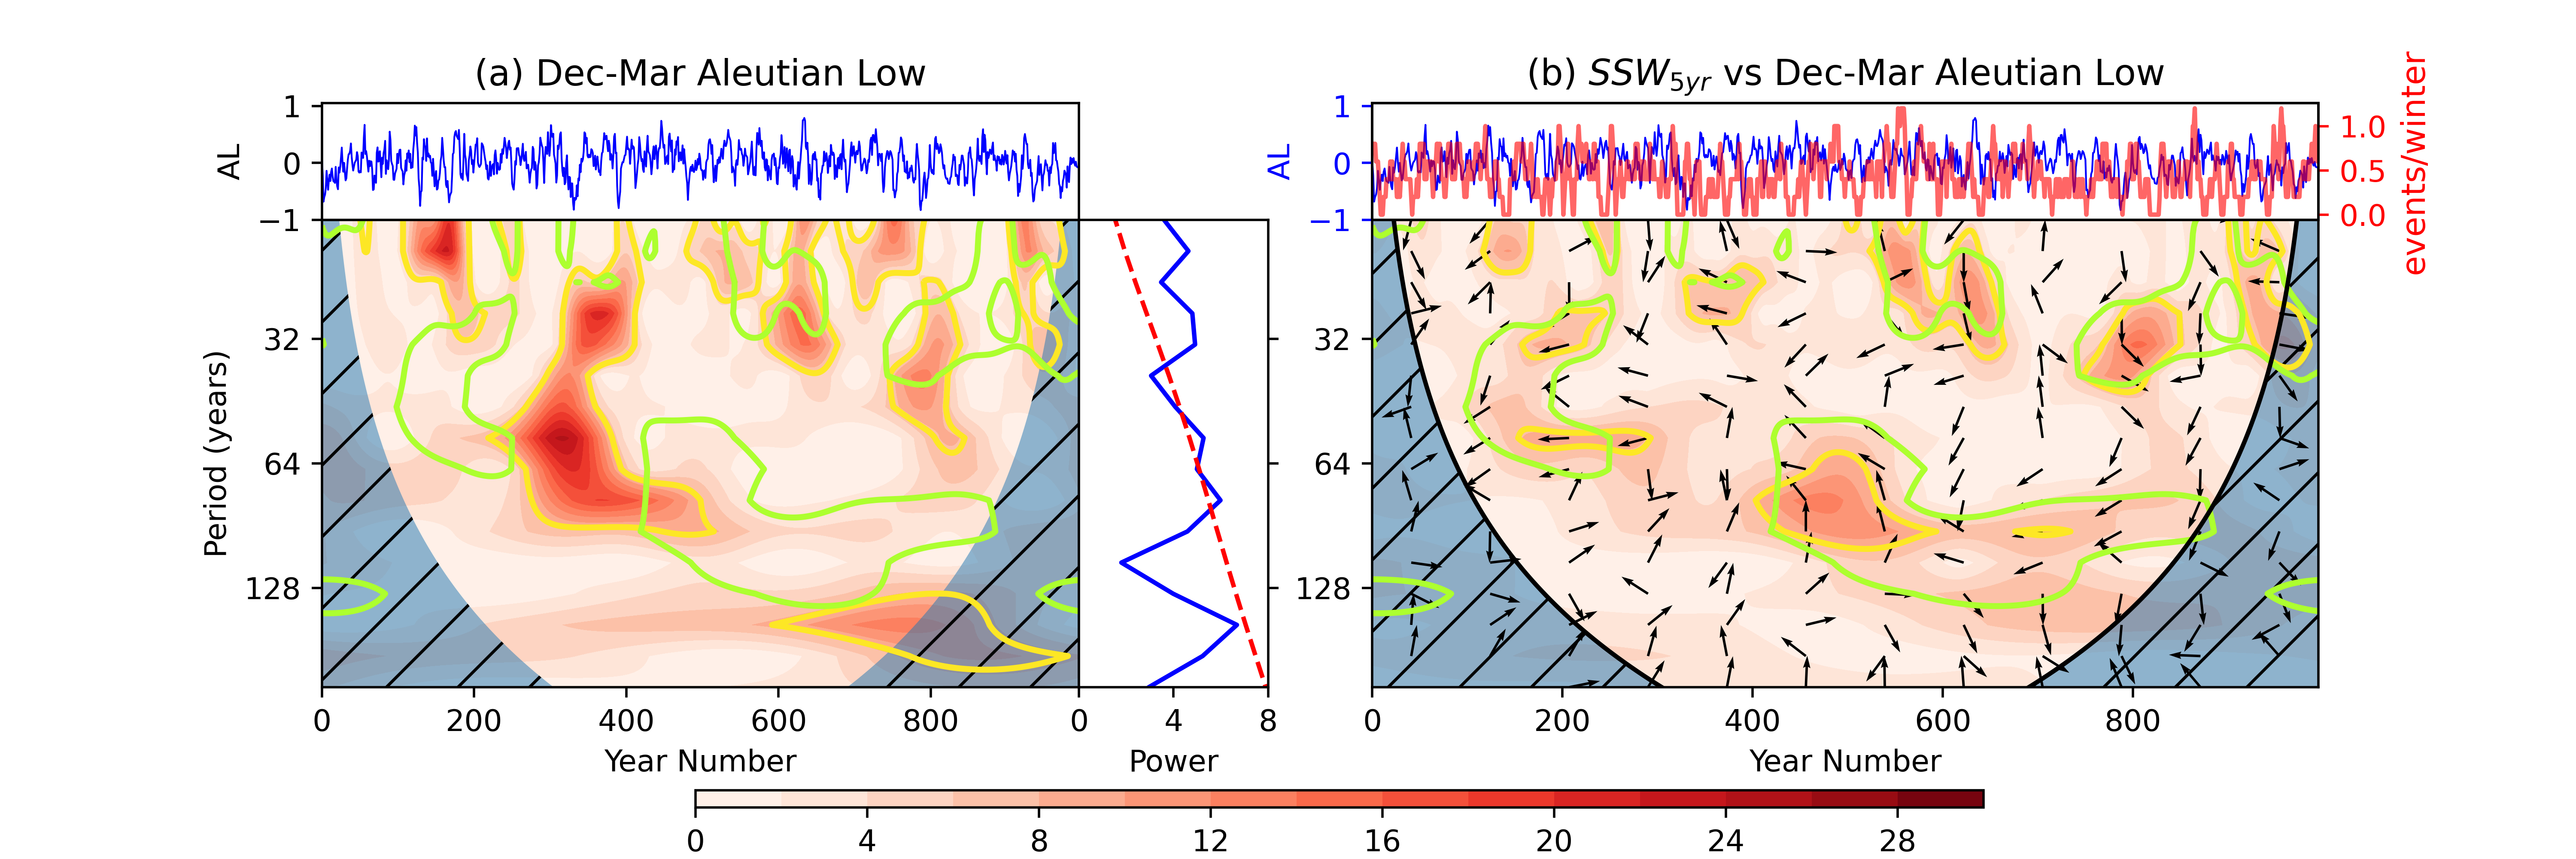
\includegraphics[width = \linewidth]{new_changed_figures/AL_wavelet_combined_new_levels.png}
\caption{As figure 8 for the Dec-Mar Aleutian Low index smoothed with a 5 year window. \textbf{a}: AL time series and associated wavelet power spectrum. \textbf{b}: Cross power spectrum between AL and $SSW_{5yr}$.}
\end{figure}
\end{center}

%---------------------------------------------------------------


\subsection{Vortex-QBO Interactions}
Despite some coincident signals between tropical SSTs, AL and $SSW_{5yr}$, long-term variability in these surface indices are unable to fully account for the  multidecadal signals in SSW frequency. An additional potential source of internally generated long-term variability may reside within the stratosphere. Studies have noted relatively long-term variations in the strength of the Holton-Tan relationship \citep{Lu2008, Lu14, OspEA10} although the cause of these variations is not well understood. In order to investigate this figure 10 shows the wavelet power spectrum of early winter (Sep-Nov) QBO winds evaluated at selected levels. Since the QBO evolves relatively slowly, employing Sep-Nov averaged winds provides a reasonable representation of the QBO and also allows us to evaluate the in-season lagged relationship between the QBO and subsequent occurrence of an SSW. There is a clear signal between 2 and 4 years for the majority of the simulation, as expected, but no prominent power at longer periods,  confirming that there is no significant long-term variability in the periodicity of the QBO winds that could explain the long-term variations in $SSW_{5yr}$ via the Holton-Tan relationship.

\begin{center}
\begin{figure}[h!]
\noindent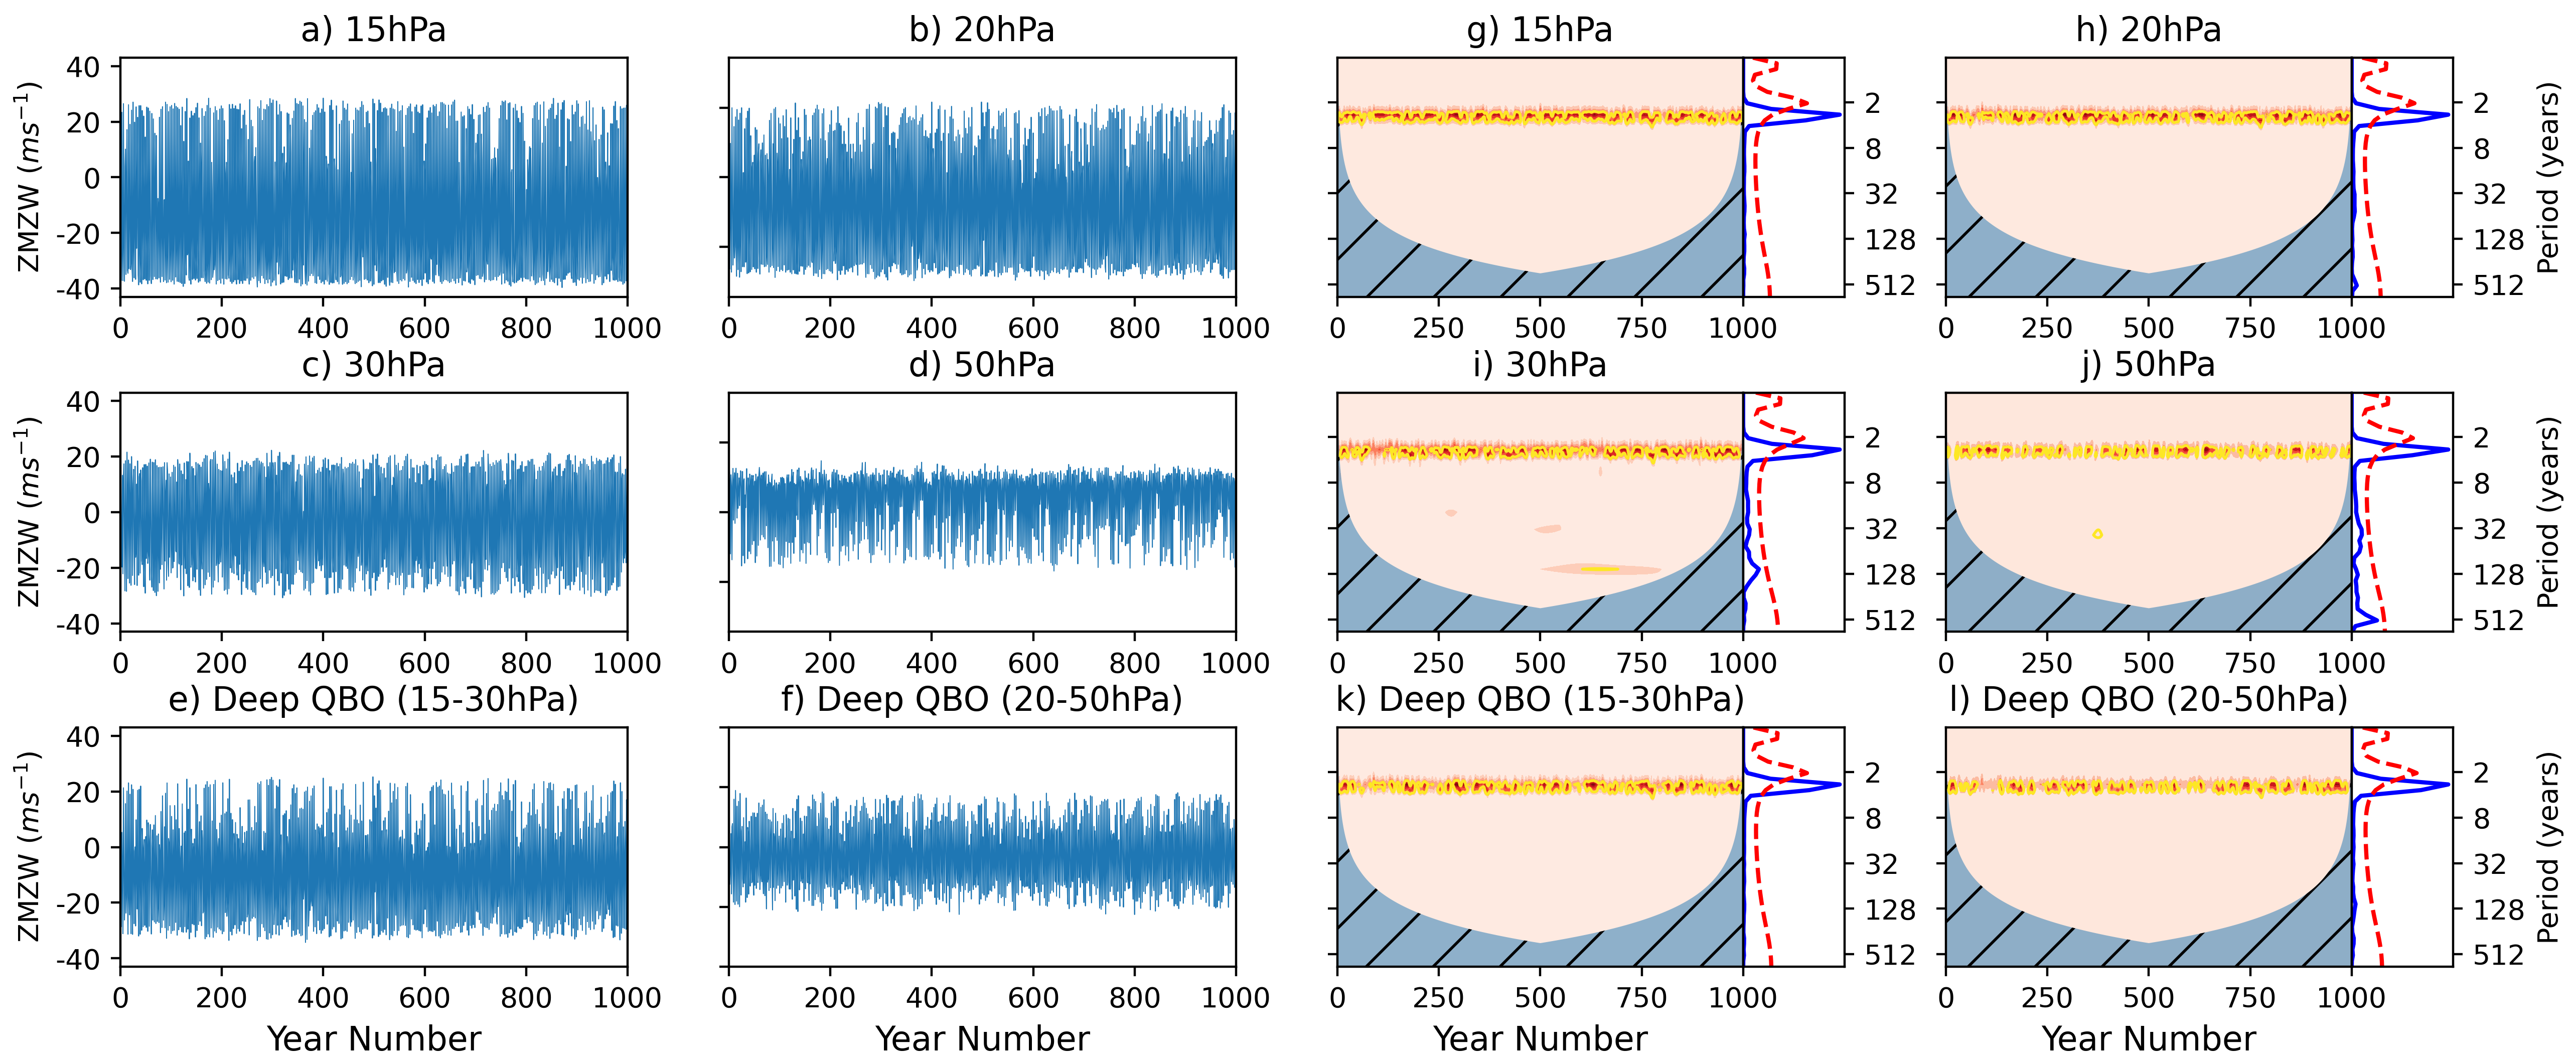
\includegraphics[width = \linewidth]{figures/QBO_levels.png}
\caption{\textbf{(a-f)}: Sep-Nov mean ZMZW averaged between 5$^\circ$S--5$^\circ$N latitude on different pressure levels (a-e) and the deep metric averaged between 15--30\,hPa (f). \textbf{(g-l)}: Wavelet power spectra for each time series shown in (a-c). Shading represents wavelet power and yellow contours indicate regions of significant power (>95\% confidence interval) compared to a background AR1 process.}
\label{fig4}
\end{figure}
\end{center}

%---------------------------------------------------------------

While the wavelet analysis technique is able to isolate and reveal frequency modulations very well it is less suited to examine amplitude modulations which are clearly evident by eye in some of the QBO index time-series. For example, both the 20 hPa and deep (15-30 hPa) QBO time series show multi-decadal variations in the magnitude of the westerly phase while the easterly phase amplitudes are relatively uniform in time. Similarly, the 50\,hPa and 30\,hPa time series show amplitude modulation predominantly in the easterly phase. This amplitude modulation can be highlighted by taking the Hilbert Transform of each QBO time-series (figure 11a-f). Wavelet analysis of the transformed QBO time series now shows significant power on multidecadal timescales (figure 11g-l). In particular, the 20\,hPa and deep QBO time-series exhibit signals coincident in time and around similar periods (60-90 years) to those observed in $SSW_5yr$. On the other hand, the QBO indices based on equatorial winds at 50\,hPa or 30\,hPa show minimal power at these periods, despite showing a strong intraseasonal HT relationship (figure 4). Given that the 15-30 hPa deep QBO  index exhibits  both multidecadal timescale variability and a strong intraseasonal HT coupling, we continue further analysis of the SSW-QBO interactions using the 15-30 hPa index. 

\begin{center}
\begin{figure}[h!]
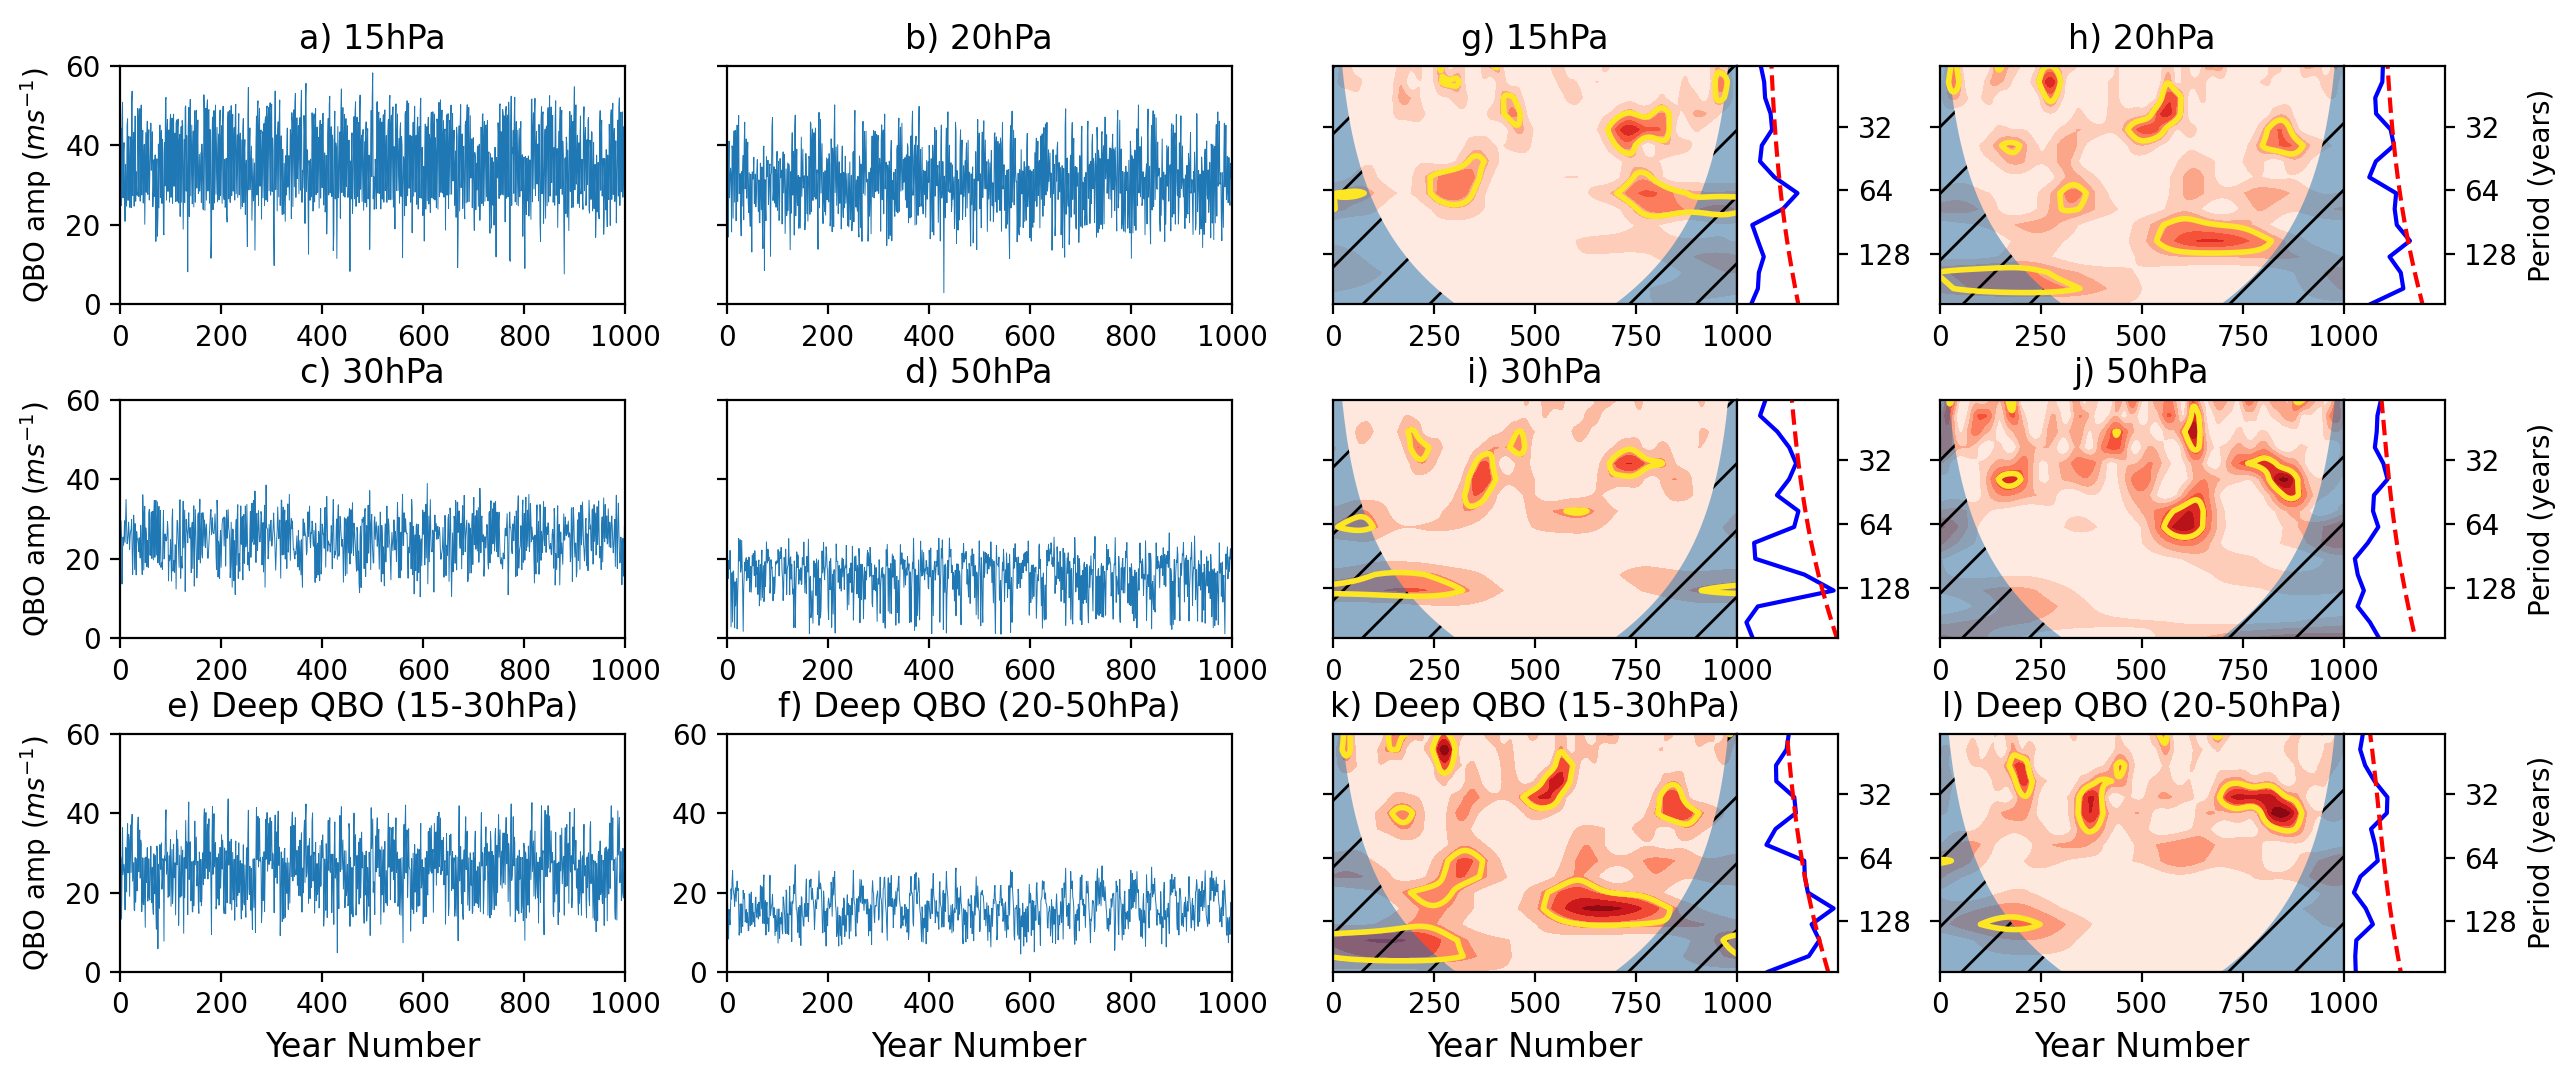
\includegraphics[width = \linewidth]{figures/QBO_levels_amp.png}
\caption{\textbf{(a-e)}: Hilbert amplitude of Sep-Nov mean ZMZW averaged between 5$^\circ$\,S--5$^\circ$\,N latitude on different pressure levels (a-e) and the deep metric averaged between 15--30\,hPa (f). \textbf{(g-l)}: Wavelet power spectra for each time series shown in (a-c). Shading represents wavelet power and yellow contours indicate regions of significant power (>95\% confidence interval) compared to a background AR1 process.}
\label{fig1}
\end{figure}
\end{center}

Wavelet analysis of the 5-year smoothed deep (15-30\,hPa) QBO amplitude modulation index (figure 12a) enhances the clarity of the long-term periodicity, showing statistically significant power at around 90 years in the interval between 500-800 years. The cross power between $SSW_5yr$ and this QBO amplitude modulation index (figure 12b) coincides extremely well with the signals observed in $SSW_5yr$ at around 90 years. There are also coincident features at other timescales, although the feature between years 450-550 at periods of 60 years is less well captured. The phase-relationship arrows in the main region of long-term variability (periods around 90 years in the interval 450-800 years) point broadly to the left ($\pi$ phase shift), indicating that the signals are approximately anti-phased (the slight downward pointing of the arrows suggests a small deviation from this lag-zero relationship and is discussed below). The anti-phase relationship is consistent with the HT relationship in which a westerly (positive) QBO anomaly corresponds to a reduction in the frequency of SSWs.


%---------------------------------------------------------------

\begin{center}
\begin{figure}[h!]
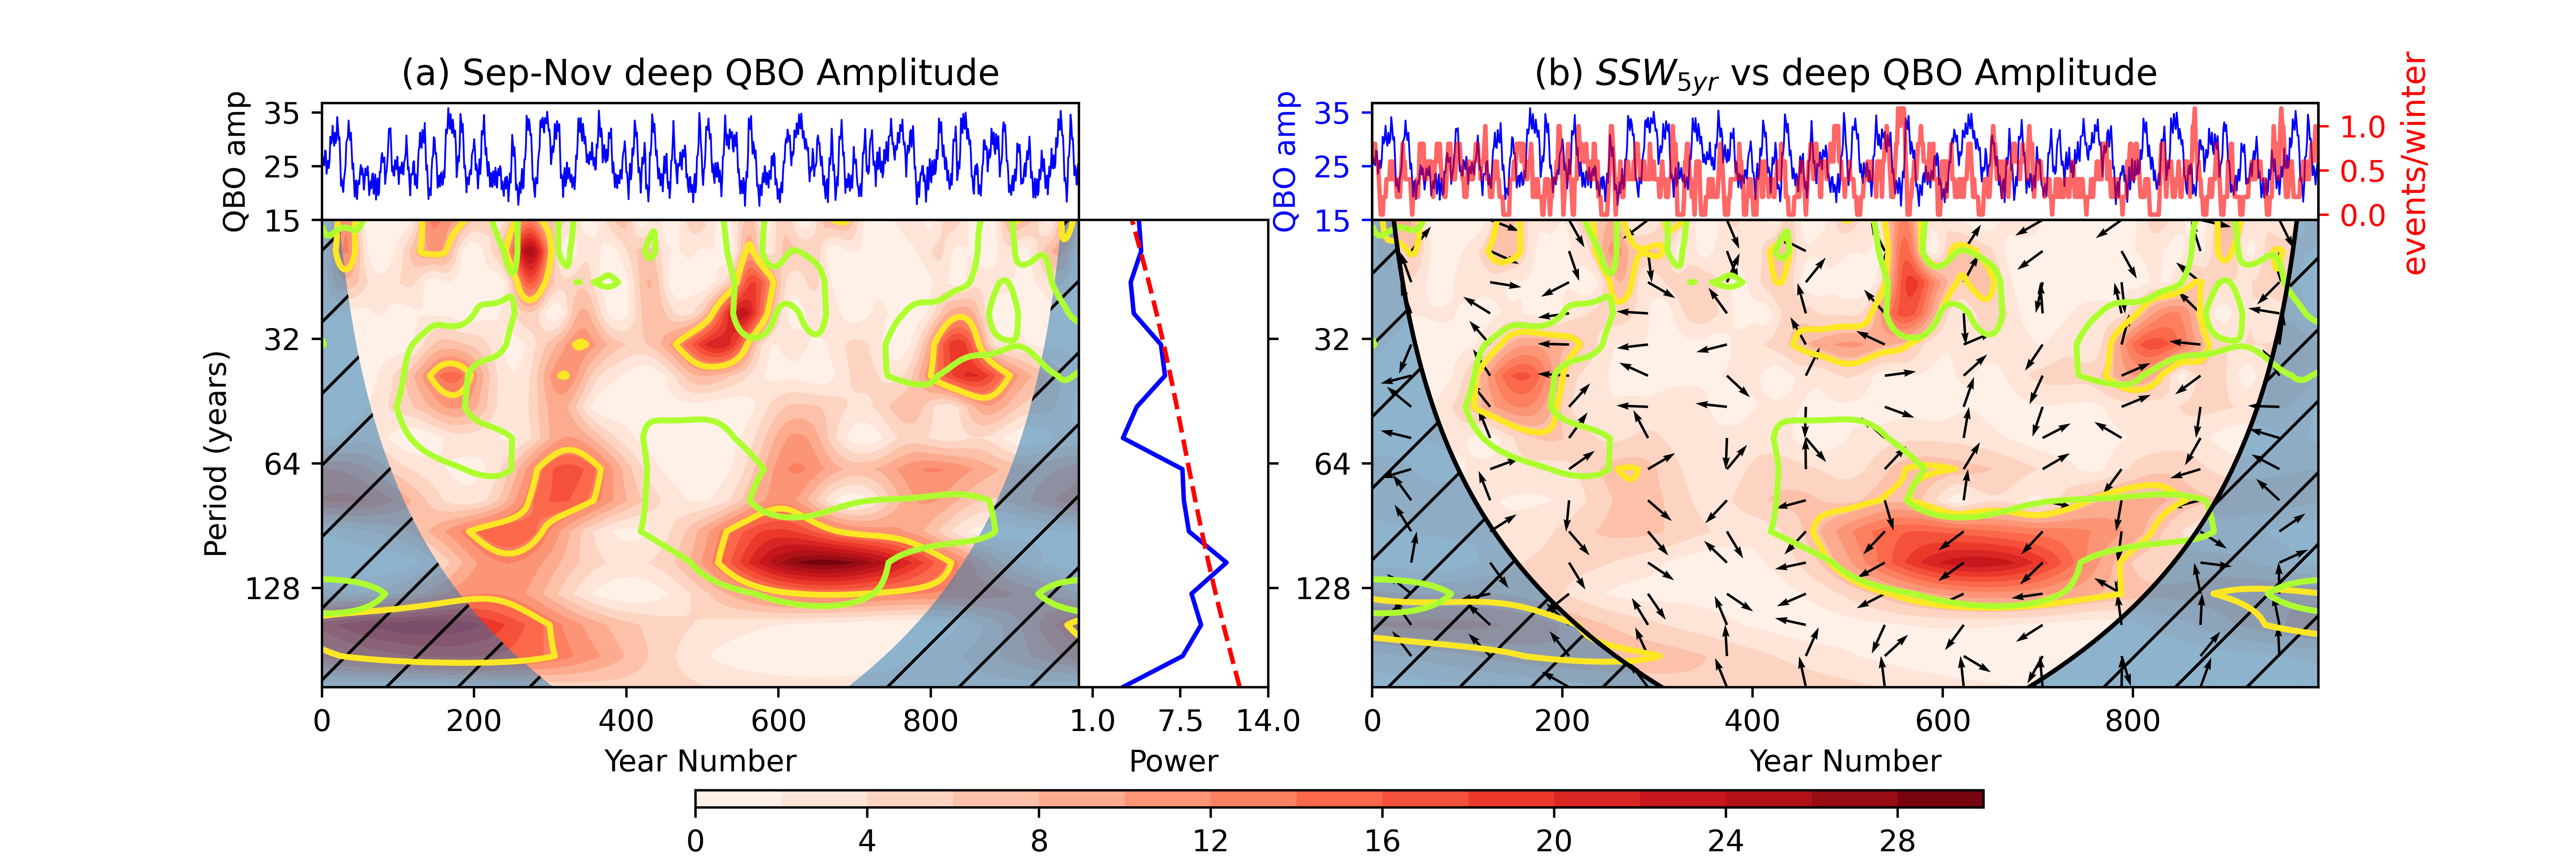
\includegraphics[width = \textwidth]{new_changed_figures/QBO_deep_amp_wavelet_combined_new_levels.png}
\caption{As figure 8 for the Sep-Nov deep QBO (15--30\,hPa) amplitude index smoothed with a 5 year window. \textbf{a}: QBO amplitude time series and associated wavelet power spectrum,\textbf{b}: Cross power spectrum between deep QBO amplitude and $SSW_5yr$.}
\end{figure}
\end{center}

In our earlier discussion we linked long-term variability in SSW frequency to the existence of extended hiatus periods, during which the vortex is relatively undisturbed with no SSW events (figure 2). The cross-spectrum analysis with deep QBO amplitude modulation suggests a possible physical interpretation involving the Holton-Tan relationship varying on longer timescales, in which a series of consecutive years that exhibit a large amplitude, deep westerly QBO in early winter leads to a series of winters with reduced SSW frequency i.e. a hiatus period. Correspondingly a series of large-amplitude deep easterly QBO years would lead to a series of consecutive-event years.

We verify the results of the wavelet analyses described above by repeating the multi-linear regression (table 1) but using the 5-year smoothed QBO, ENSO and AL indices to measure their  relative contributions to the 5-year smoothed  $SSW_5yr$ time-series. The resulting regression coefficients for the deep QBO amplitude and AL remain significant at the 95\% level, although the AL's contribution remains small and close to the significance boundary. The coefficient for ENSO3.4 is not significant, suggesting that the connection between ENSO and the vortex variability is dominated by timescales less than 5 years. If we further isolate multi-decadal signals by fourier filtering each timeseries, so that only periodicities longer than 60 years are retained, the ENSO3.4 coefficient is near 0 while the deep QBO amplitude signal is near -0.2. This is consistent with our wavelet analysis which suggest a dominant role for QBO amplitude variations on these long timescales. The AL coefficient remains significant but smaller than that of the QBO (and outside error ranges). For completeness, we repeated the regression analysis using a 5-year smoothed PDO index instead of the AL but there was no significant change in the coefficients (not shown). This is consistent with the fact that the AL and PDO indices exhibit similar spectra and there is a high correlation between them (-0.45 unfiltered and -0.68 filtered), as also found by \cite{Mantua_1997} and \cite{Rodionov2005}. 

\begin{table}
\centering
\begin{tabular}{|p{3cm}||p{3cm}|p{3cm}|}
 \hline
 \multicolumn{3}{|c|}{SSW$_{5yr}$ regression}\\
 \hline
 Regression Variable& Coefficient& p value\\
 \hline
 ENSO3.4  & -0.0127$\pm$0.032& 0.688\\
 AL  &   -0.072$\pm$0.021  & 0.046\\
 deep QBO amp &-0.124$\pm$0.031&0.0001\\
 \hline
\end{tabular}
\begin{center}
\caption{Summary of results from multi-linear regression analysis of SSW$_{5yr}$.} 
\end{center}
\end{table}

\begin{table}
\centering
\begin{tabular}{|p{3cm}||p{3cm}|p{3cm}|}
 \hline
 \multicolumn{3}{|c|}{Filtered (>60 year periods) SSW$_{5yr}$ regression}\\
 \hline
 Regression Variable& Coefficient& p value\\
 \hline
 ENSO3.4  &   $\sim$0$\pm$0.01  & $\sim$1\\
 AL & -0.0794$\pm$0.03& 0.042\\
 deep QBO amp &-0.199$\pm$0.01&0.00003\\
 \hline
\end{tabular}
\begin{center}
\caption{Summary of results from multi-linear regression analysis of a fourier filtered  version of SSW$_{5yr}$ retaining power corresponding to periods greater than 60 years.}  
\end{center}
\end{table}


To further clarify the role of the QBO, we note that an examination of figure 10 shows that the majority of the long-term amplitude variability in the 15-30 hPa deep QBO index lies in the amplitude of the westerly phase (the easterly phase amplitude is relatively constant with time). Also, as noted earlier, the simulation exhibits more hiatus intervals than consecutive-event intervals, which suggests that the observed long-term variability may arise primarily from the westerly QBO phase. To explore this hypothesis, we isolate the SSW  hiatus intervals by modifying the $SSW_5yr$ time-series in the following way. All SSW rates above 0.54 events per season (the climatological mean) are re-set to 0.54 thereby removing variability in 5 year intervals that exhibit anomalously high SSW rates. Figure 13 shows the cross power spectrum between this modified $SSW_5yr$ time-series and the time-series of deep QBO amplitude. It retains significant cross power within the portion of significant $SSW_5yr$ power (figure 13 green contours) when compared with figure 12b in which the full time-series is used and also shows a phase relationship significantly closer to anti-phased (i.e. pointing to the left). This is further support that the deep QBO - SSW relationship  on these long timescales in the model arises primarily from the SSW hiatus periods. 


\begin{center}
\begin{figure}[h!]
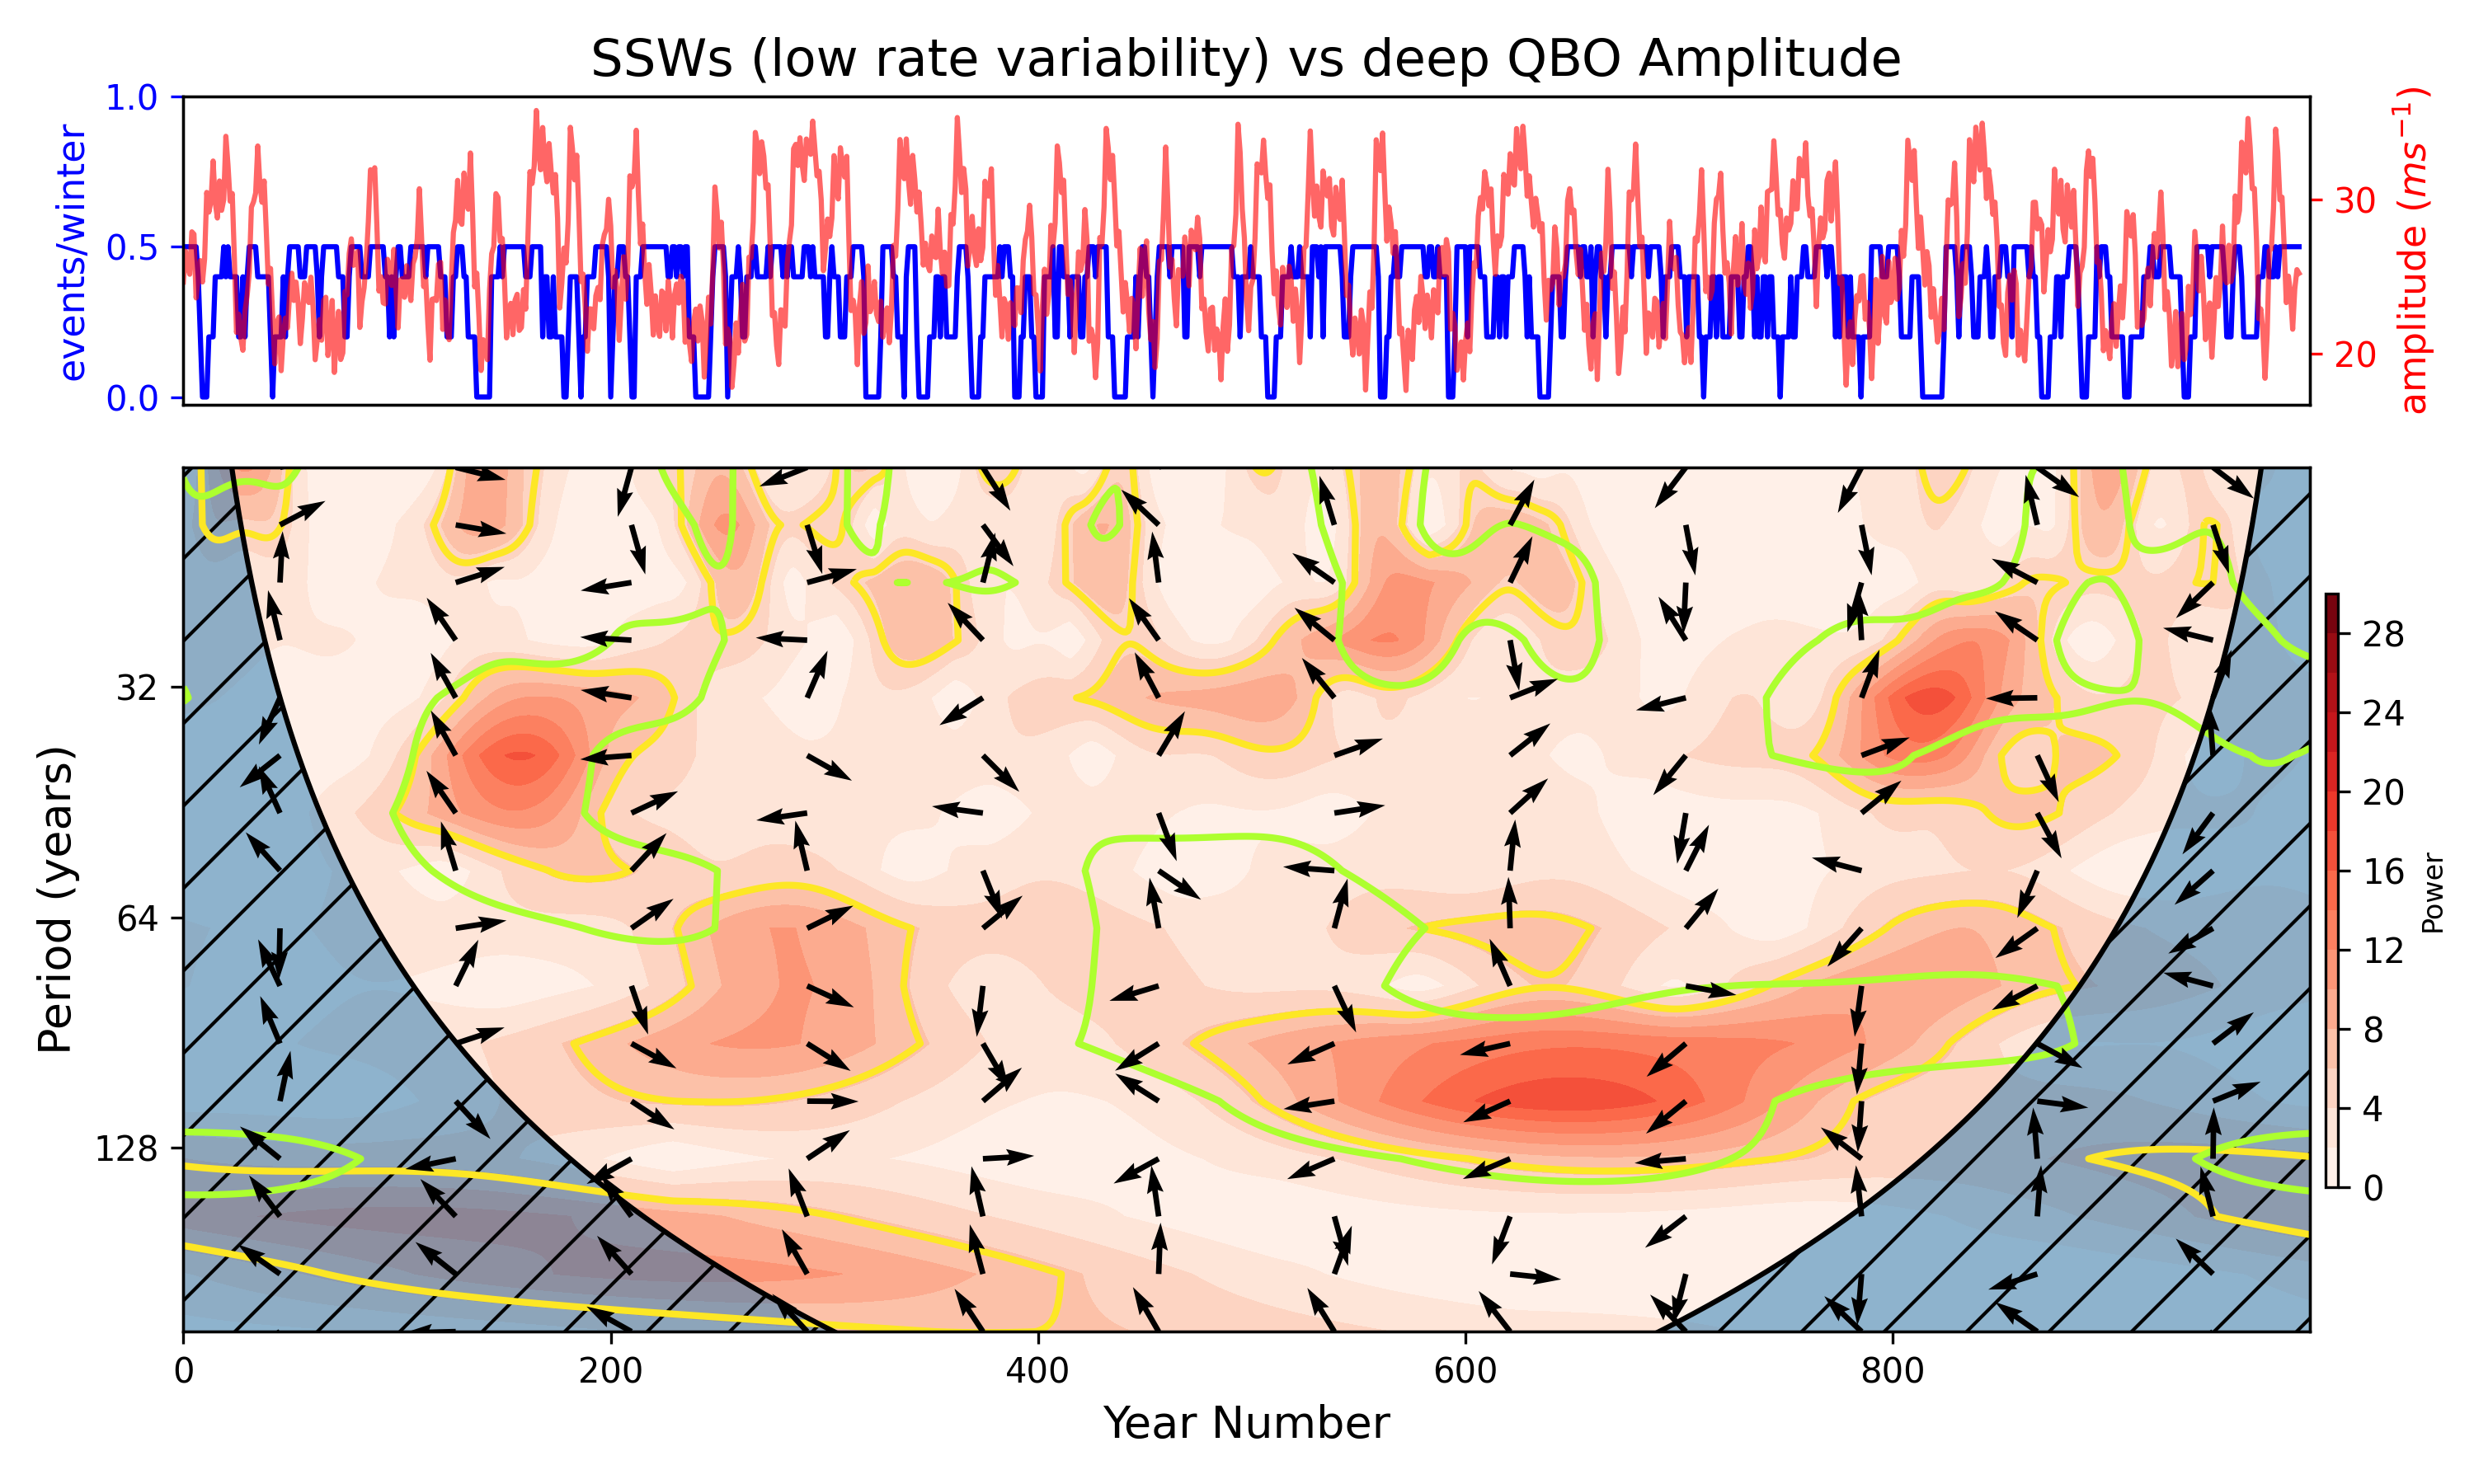
\includegraphics[width = 0.8\linewidth]{new_changed_figures/cross_power_SSWs_low_rates_vs_QBO_amplitude_modulation_5yr_mean_new_levels.png}
\caption{\textbf{Top}: $SSW_{5yr}$ time series with variability in high SSW rate intervals removed by setting all rates above the climatological mean (0.54 events per season) to the mean (blue) and Sep-Nov deep QBO Hilbert Amplitude index smoothed with a 5 year window (red). \textbf{Bottom}: Cross wavelet power spectrum between the two time series.}
\label{fig1}
\end{figure}
\end{center}

An obvious question is whether this sensitivity to deep QBO westerlies that we find in the model is also present in the real atmosphere. Examination of the ERA-Interim dataset shows limited support. Some winters in the 1990s are characterised by anomalously westerly Sep-Nov equatorial winds which are vertically coherent between the 15 and 30\,hPa levels. However this effect is intermittent and does not span the whole interval of the 1990s during which SSWs were markedly absent in the observational record (not shown). On the other hand, a mini hiatus that was present in the mid 2010s is associated with 3 years of deep westerly anomaly in the QBO. Overall, it is clear that the relationship, if present in the real atmosphere, is likely obscured by other factors including greenhouse gas increases and volcanic eruptions and the observational dataset is too short to provide useful validation for these long timescale variations.  

 
\section{Summary and Discussion}

In this study, we have examined variability in the appearance of hiatus and intervals of consecutive SSWs in a 1000-yr pre-industrial control simulation of the UK Earth System Model. While there is much observational evidence for an impact of SSWs on the underlying tropospheric weather and climate, their multi-decadal variability and the associated forcing mechanisms are not well understood due to the short observational record. Analysis of long climate model simulations is currently the only available tool for understanding this variability. 

We found realistic decadal and multi-decadal variability in the model, with hiatus intervals of 10 years or more in which no SSWs occurred, similar to the observed SSW record in the 1990s \citep{Pawson1999, Shindell1999} and also intervals of consecutive-event periods in which at least one SSW occurred every year, as observed in the early 2000s \citep{Manney2005}. A 5-yr smoothed representation of SSW frequency ($SSW_{5yr}$) was found to vary periodically for approximately 450 years of the 1000-yr simulation with maxima in wavelet power corresponding to periodicity of around 60-90 years. 

A possible tropical SST source of this long-term variability was investigated. Wavelet and cross-spectrum analyses were performed using a variety of different tropical SST indices, including the ENSO 3.4 index, and also an index of the strength of the Aleutian Low (AL) which is linked to large-scale planetary wave forcing of the winter stratosphere. While all of these indices displayed long-term variability, some of which overlapped with the periodicity and time intervals seen in the $SSW_{5yr}$ spectrum, none of them could fully account for the extended 450 year interval of significant power at 60-90 years seen in the $SSW_{5yr}$ spectrum.

A second possible source of long-term variability involving variations in the QBO was also investigated. A range of QBO indices were considered, including the standard approach of using equatorial winds at a specified pressure level e.g. 50 hPa and also a 'deep QBO'  index which takes the average QBO wind over 15-30 hPa, designed to capture the degree of vertical coherence in the QBO winds (following \cite{Gray2018} and \cite{Andrews2019}). A straightforward wavelet analysis of these QBO indices reveals no power at periodicity longer than 2-4 years. However, while there is evidently no long-term variability in the frequency of the QBO, visual examination of the QBO time series clearly shows the presence of  long-term variability in the QBO amplitudes. A measure of this amplitude modulation was extracted by taking the Hilbert Transform of the QBO index. Wavelet analysis of the amplitude variations from the Hilbert Transform of the QBO indices showed long-term periodicity matching that seen in the $SSW_{5yr}$ wavelet analysis. In particular, the deep QBO index exhibited significant signals coincident with those in $SSW_{5yr}$ corresponding to periodicities of around 90 years. This overlap accounted for nearly all 450 years of SSW variability present on the 90 year timescale. Regression analysis of 5 year smoothed and filtered indices confirmed the contribution of the deep QBO amplitude to variability in SSWs on timescales greater than 60 years. 

Our analysis has therefore revealed an unexpected relationship between the strength and vertical coherence of the QBO and long-term variability in the frequency of SSWs. The relationship was found to be particularly sensitive to the QBO westerly phase. Extended periods of deep westerly QBO phases were associated with hiatus periods with few or no SSWs, consistent with the Holton Tan relationship. While this result appears compelling, it should be noted that the model showed some biases in its QBO associated with the period and descent rate of shear zones. The extended period of close to 3 years could introduce an element of phase locking between the QBO and seasonal cycle causing winter months to occur preferentially in one QBO phase over the other (evident from figure 5, legends). This may influence QBO-vortex coupling. However, these biases are common in modern GCMs \citep{Bushell2020} and the pi-control remains the most effective tool for studying multi-decadal variability in the stratosphere.
Recent work has also shown a large degree of inter-model variability exists in representations of the QBO as well as SSWs \citep{Bushell2020,Ayarz2020} so it is possible the result from this study is model dependant. Additional analysis of long simulations from different models is required to verify these results. 

Combining the results of all these analyses, our overall  conclusion is that multi-decadal variability in SSW frequency in the model is primarily accounted for by long term variability in QBO-SSW coupling, particularly at periodicities of around 90 years and, to a lesser extent, by variability in the intensity of the Aleutian Low at periodicities around 60 years, although coherence with the AL signals is far less persistent than with the QBO. Given the observed impact of SSWs on the underlying tropospheric weather and climate, improved understanding of the source and mechanisms of long-term variability in QBO-SSW interactions is likely to help improve future seasonal weather forecasts and decadal-scale climate predictions. The precise nature of QBO-SSW interaction mechanisms are still not fully understood \citep{Anstey2014}. While the importance of wave-mean flow interactions is widely recognised, further studies are required to explore the relevance and usefulness of the deep QBO index highlighted in this study, that identifies a vertically coherent QBO phase. It appears to be especially relevant to long-term QBO-SSW interactions during the QBO-W phase. 

Further exploration of the source of the long-term variability in amplitude of the QBO-W phase is also required. While a direct influence of tropical SSTs on long-term variability in SSW frequency has not been supported by this study there may nevertheless be an important teleconnection via the QBO, in which the SSTs influence the QBO which subsequently influences the SSW frequency via the Holton Tan relationship. Initial investigation through cross spectrum analysis of the deep QBO index with ENSO and selected SST indices shows some contribution from each of the regions (supp figures A6 and A7), not surprisingly because of the tropical source of equatorial waves that are known to drive the QBO. A closer examination of the precise nature of forcing of the QBO-W phase in the model, in terms of Kelvin and gravity wave forcing would be helpful (but outside the scope of this study). 

Time series analysis such as those presented here can highlight associations between modes of variability but are less able to determine causality. Where possible we have selected indices that confirm well-known in-season causality, such as an early winter QBO index compared with a mid-winter SSW index, but determining causality on longer timescales is much more difficult. Well designed climate model experiments can help, for example to eliminate SST variability by using an atmosphere-only model with climatological SST forcing which could help to identify whether the QBO-W amplitude variations are externally forced by the SSTs or whether they are internally-driven (e.g. through nonlinear interactions within the stratosphere).  Similarly, there are other potentially important teleconnections that have not been examined in this study, for example the possible role of North Atlantic and/or North Pacific blocking, and other potential sources of long-term variability such as the Pacific North America (PNA) pattern and the Atlantic Multidecadal Variability (AMV) index. The climate system is extremely complex, with many different interactions between these modes of variability. The climate system is also clearly non-stationary, as evident in our simulation where the QBO-SSW interaction shows power at periodicities of 60-90 years for 450 years but is absent in the early half of the simulation. While this complexity means that it is extremely challenging to disentangle the influences or to attribute causality, improved understanding of individual links in this complex system, such as the relationship between the QBO and SSWs, will nevertheless contribute to improved understanding of the whole complex system.   

%\raggedright

\subsubsection*{\normalsize\normalfont\textit{Data availability. }ERA-Interim reanalysis data are available from the Copernicus Climate Change Service Climate Data Store \newline(CDS, https://climate.copernicus.eu/climate-reanalysis,
C3S, 2017). Data from the UKESM simulation used in this study are available from the Earth System Grid Federation of the Centre for Environmental Data Analysis (ESGF-CEDA;https://esgf-index1.ceda.ac.uk/projects/cmip6-ceda/,WRP,2019, last access: 6 Oct 2020).}

\subsubsection*{\normalsize\normalfont\textit{Author contributions. } OBDM conducted the analyses, and LJG and SO directed the research. All authors were fully involved in preparing and revising the text.}

\subsubsection*{\normalsize\normalfont\textit{Competing interests. }The authors declare that they have no conflict of interest.}

\subsubsection*{\normalsize\normalfont\textit{Financial support. }LJG and SO acknowledge funding from the UK Natural Environment Research Council (NERC) through the National Centre for Atmospheric Science (NCAS) ACSIS project (NE/N018001/1) and the NERC Belmont-Forum grant GOTHAM (NE/P006779/1). OBDM gratefully acknowledges support from the Oxford DTP in Environmental Research (NE/L002612/1)}

\subsubsection*{\normalsize\normalfont\textit{Acknowledgements. }The authors would like to thank their respective funding bodies as well as Tim Woollings, Antje Weisheimer and Chris O'Reilly for useful discussions. We also give thanks to the UKESM1 team who have worked to develop and run the model used in this study as well as make the data available. In particular, Colin Jones, Jeremy Walton, Alistair Sellar and Till Kuhlbrodt.}


\bibliographystyle{copernicus}
\bibliography{paper_bibliography} 

\newpage
\section{Appendix A}
\appendix
\appendixfigures  %% needs to be added in front of appendix figures

%\section{Supplementary Material STARTS HERE}
\begin{center}
\begin{figure}[h!]
\noindent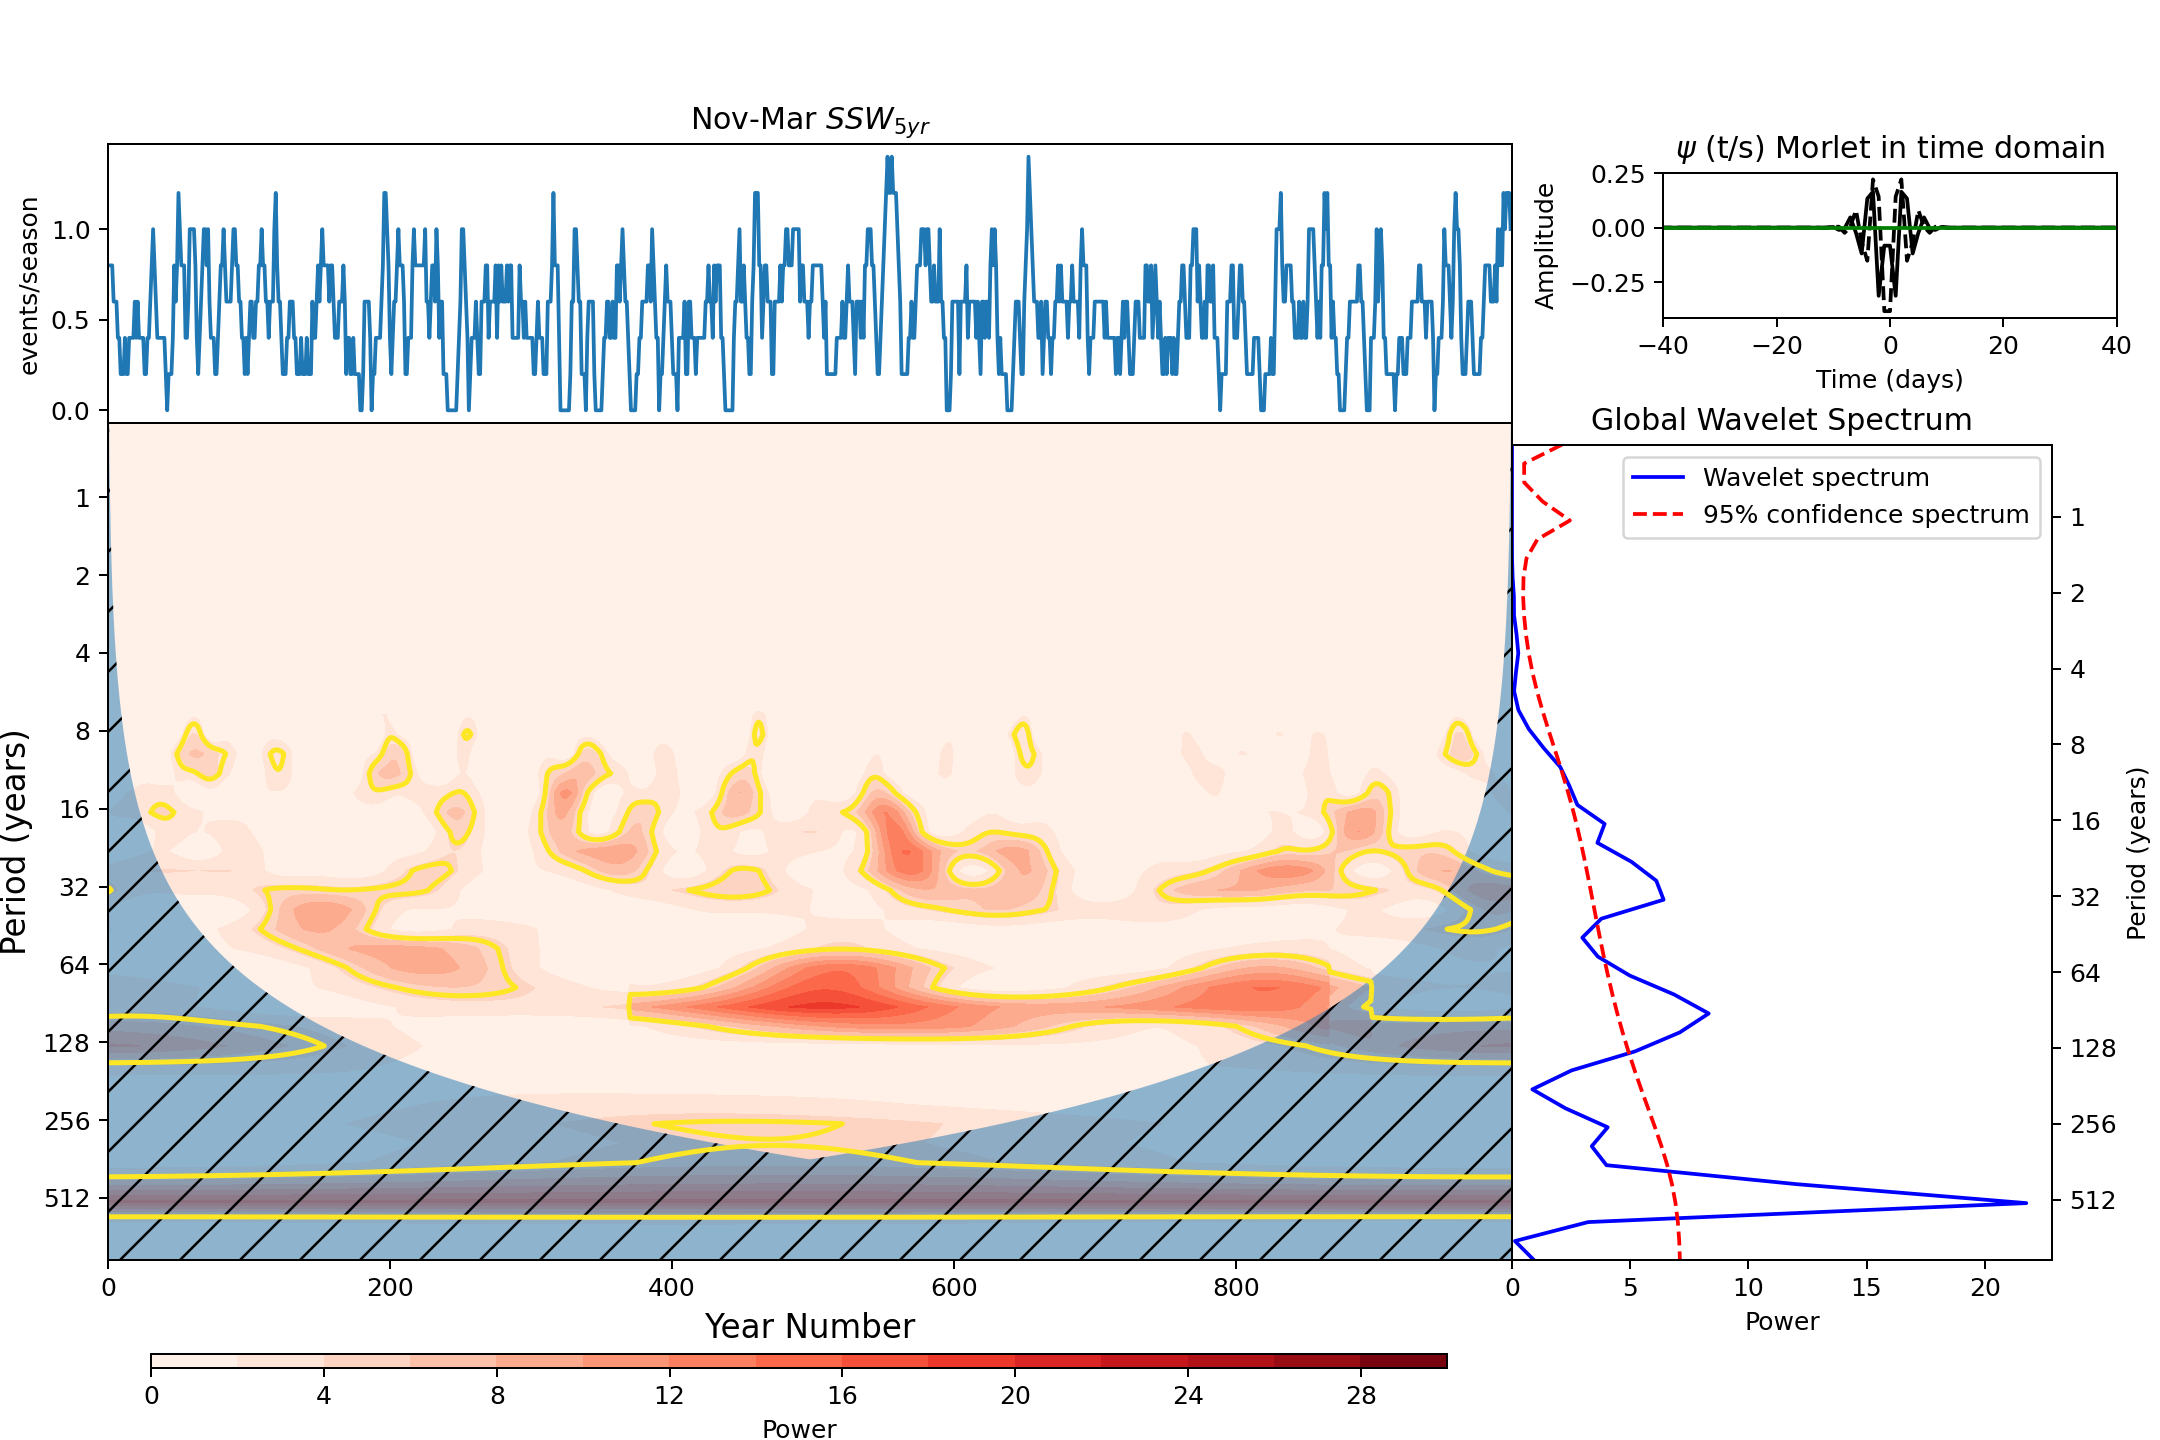
\includegraphics[width = 0.8\linewidth]{new_changed_figures/SSW_wavelet_5_yr_fig3_new_levels_NDJFM.png}
\caption{\textbf{Top left}: SSW events per Nov-Mar season in UKESM smoothed using a 5 year running mean. \textbf{Bottom left}: Wavelet power spectrum of time series in top left. Hatching represents area outside the cone of influence in which edge effects are significant and power should not be considered. Yellow contours represent 95\% confidence level assuming mean background AR1 red noise. \textbf{Top Right}: Morlet wavelet used for the wavelet transform in the time domain. \textbf{Bottom right:} Global power spectrum, the wavelet power averaged over the whole simulation, and global 95\% confidence spectrum.}
\label{fig3}
\end{figure}
\end{center}

\begin{center}
\begin{figure}[h!]
\noindent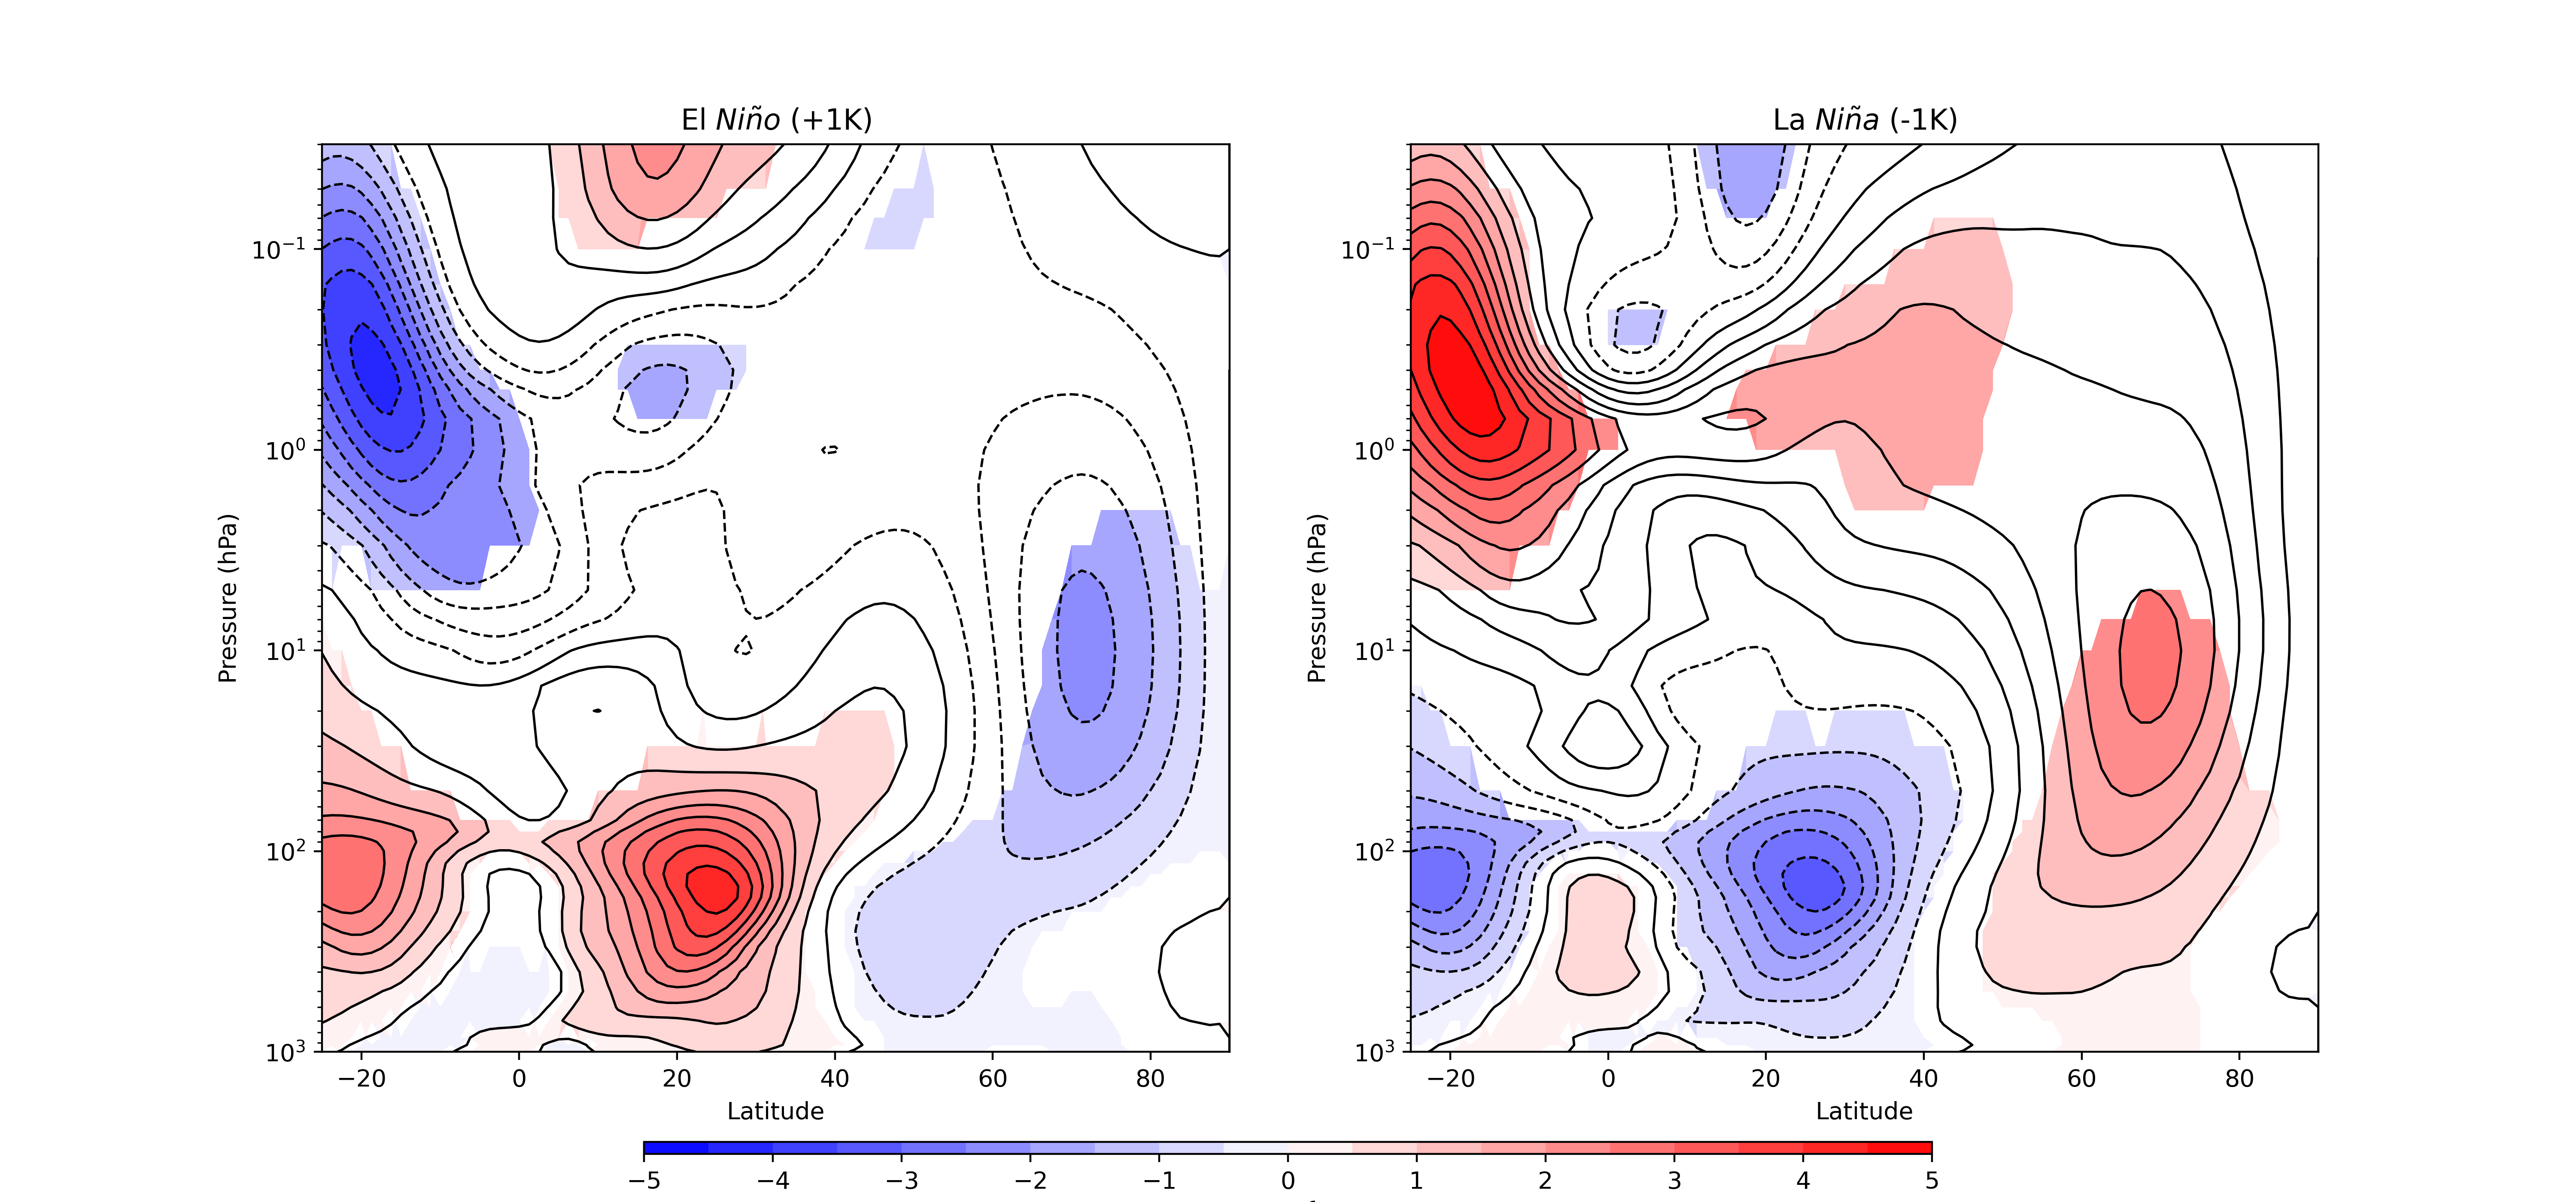
\includegraphics[width = \linewidth]{new_changed_figures/ZMZW_ENSO_phase_1K.png}
\caption{Dec-Mar ZMZW anomaly composites for positive (El Ni\~{n}o) and negative (La Ni\~{n}a) phases of the ENSO3.4 index evaluated in Sep-Nov. The phase of ENSO3.4 is defined as an SST anomaly of greater magnitude than 1K. Coloured shading indicates anomalies significant above the 95\% confidence level under a 2 tail student’s t-test.}
\label{fig3}
\end{figure}
\end{center}


\begin{center}
\begin{figure}[h!]
\noindent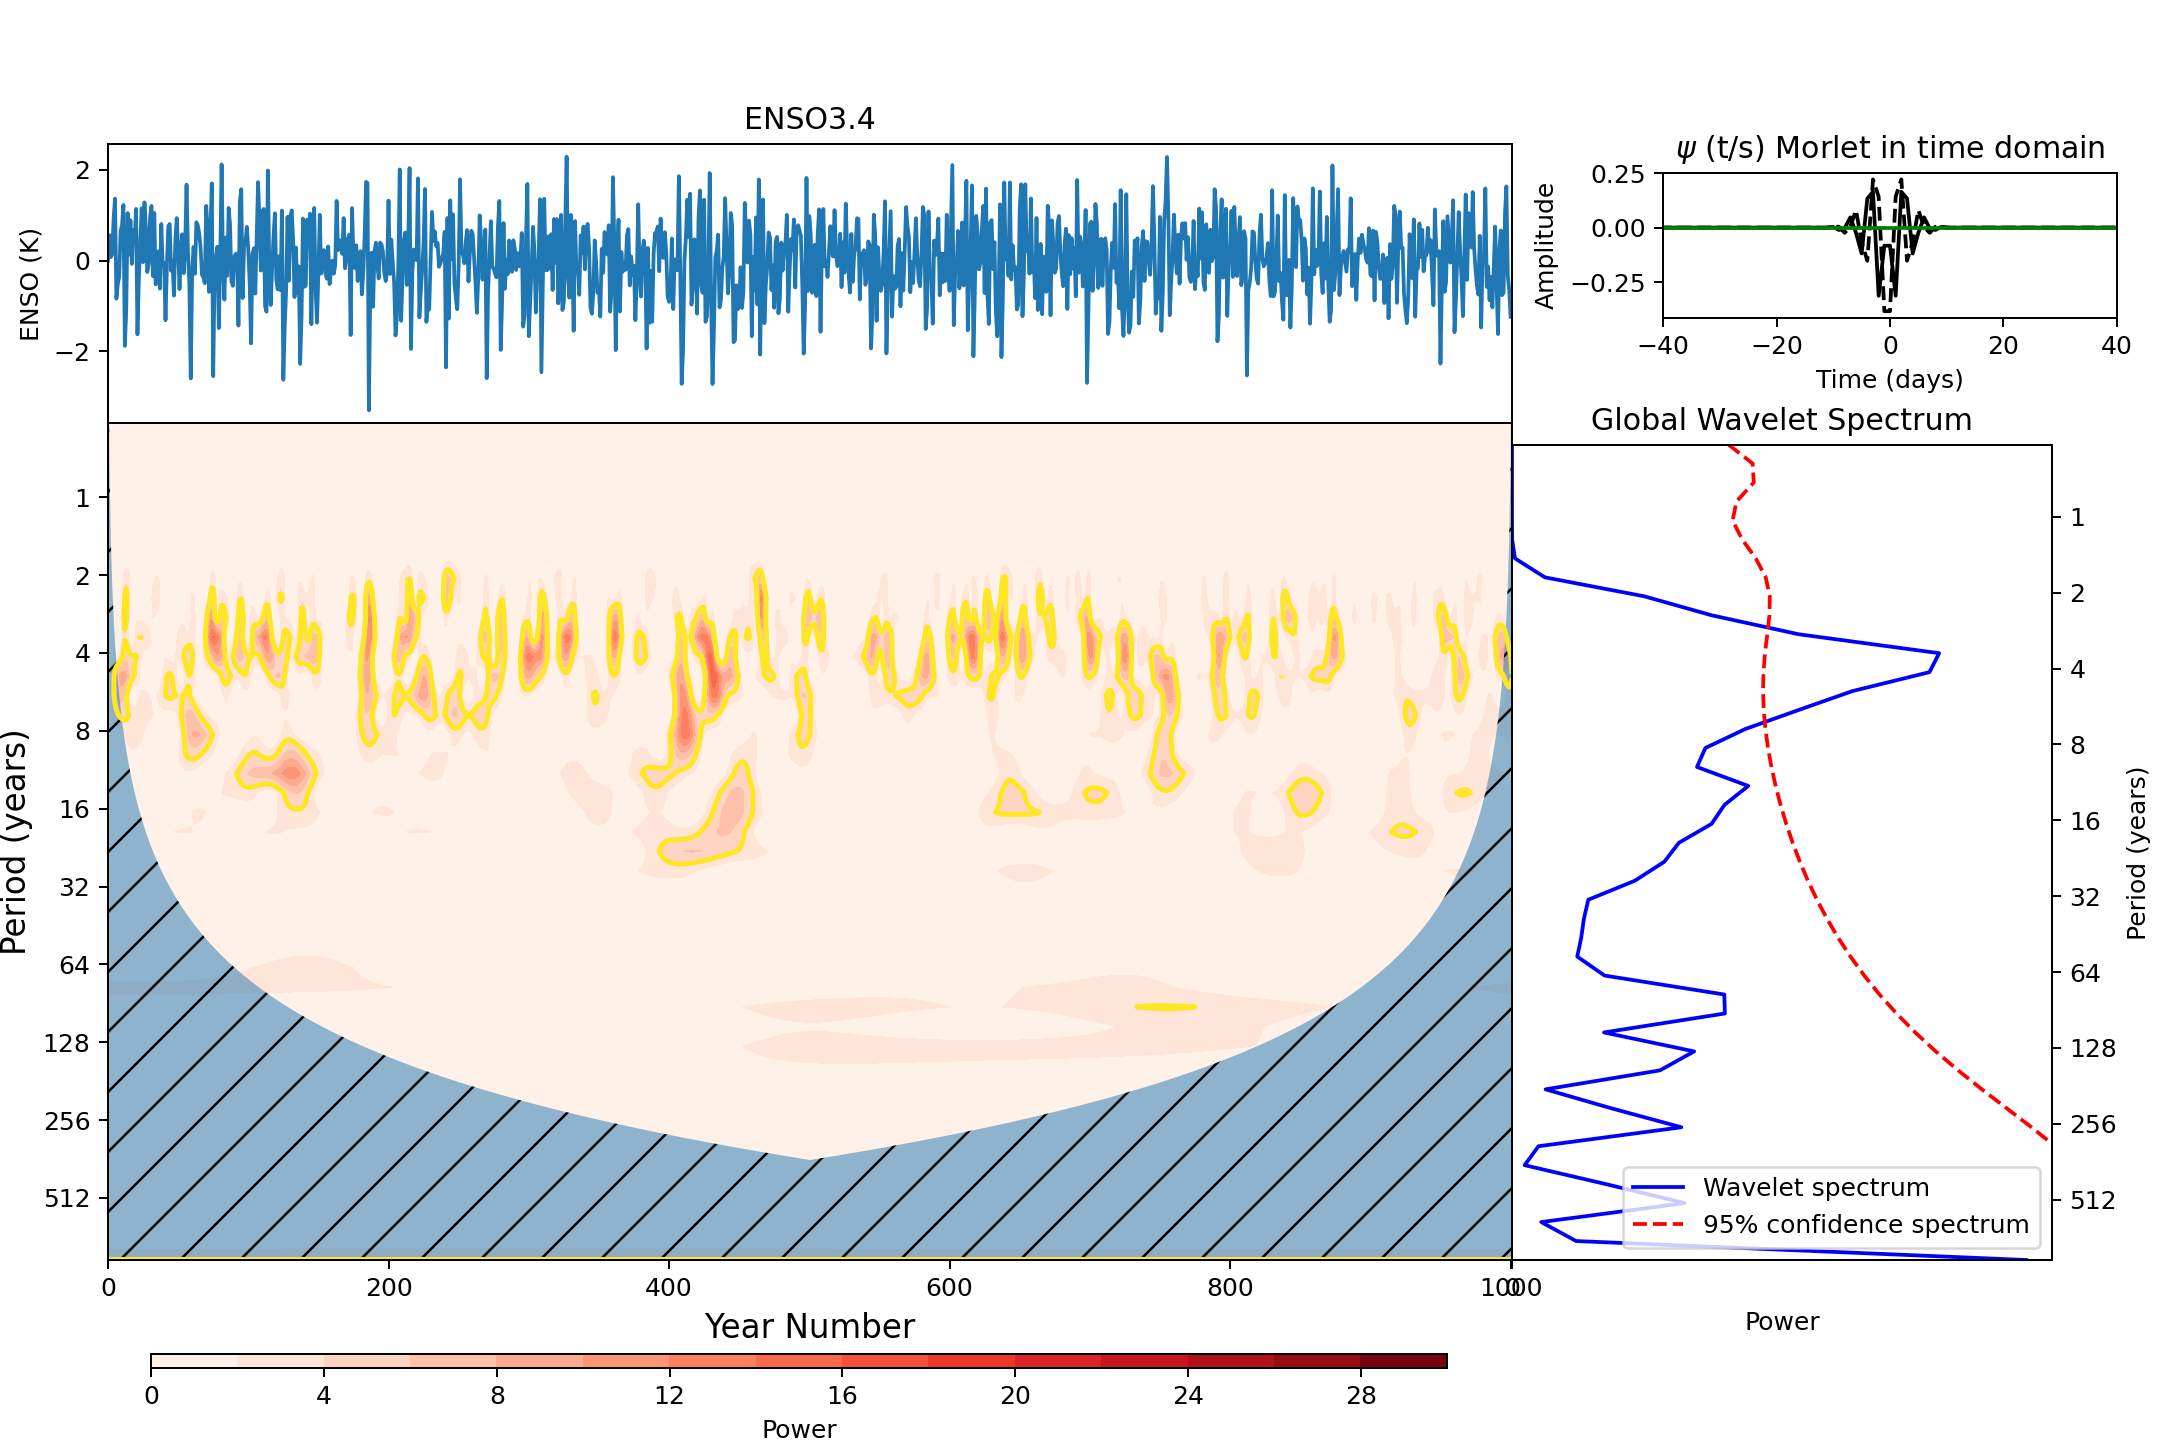
\includegraphics[width = \linewidth]{new_changed_figures/ENSO_wavelet_new_levels.png}
\caption{\textbf{Top left}: Sep-Nov ENSO3.4 index from the UKESM pi-control simulation. \textbf{Bottom left}: Wavelet power spectrum of time series in top left. Hatching represents area outside the cone of influence in which edge effects are significant and power should not be considered. Yellow contours represent the 95\% confidence level assuming mean background AR1 red noise. \textbf{Top Right}: Morlet wavelet used for the wavelet transform in the time domain. \textbf{Bottom right:} Global power spectrum, the wavelet power averaged over the whole simulation, and global 95\% confidence spectrum.}
\label{fig3}
\end{figure}
\end{center}

\begin{center}
\begin{figure}[h!]
\noindent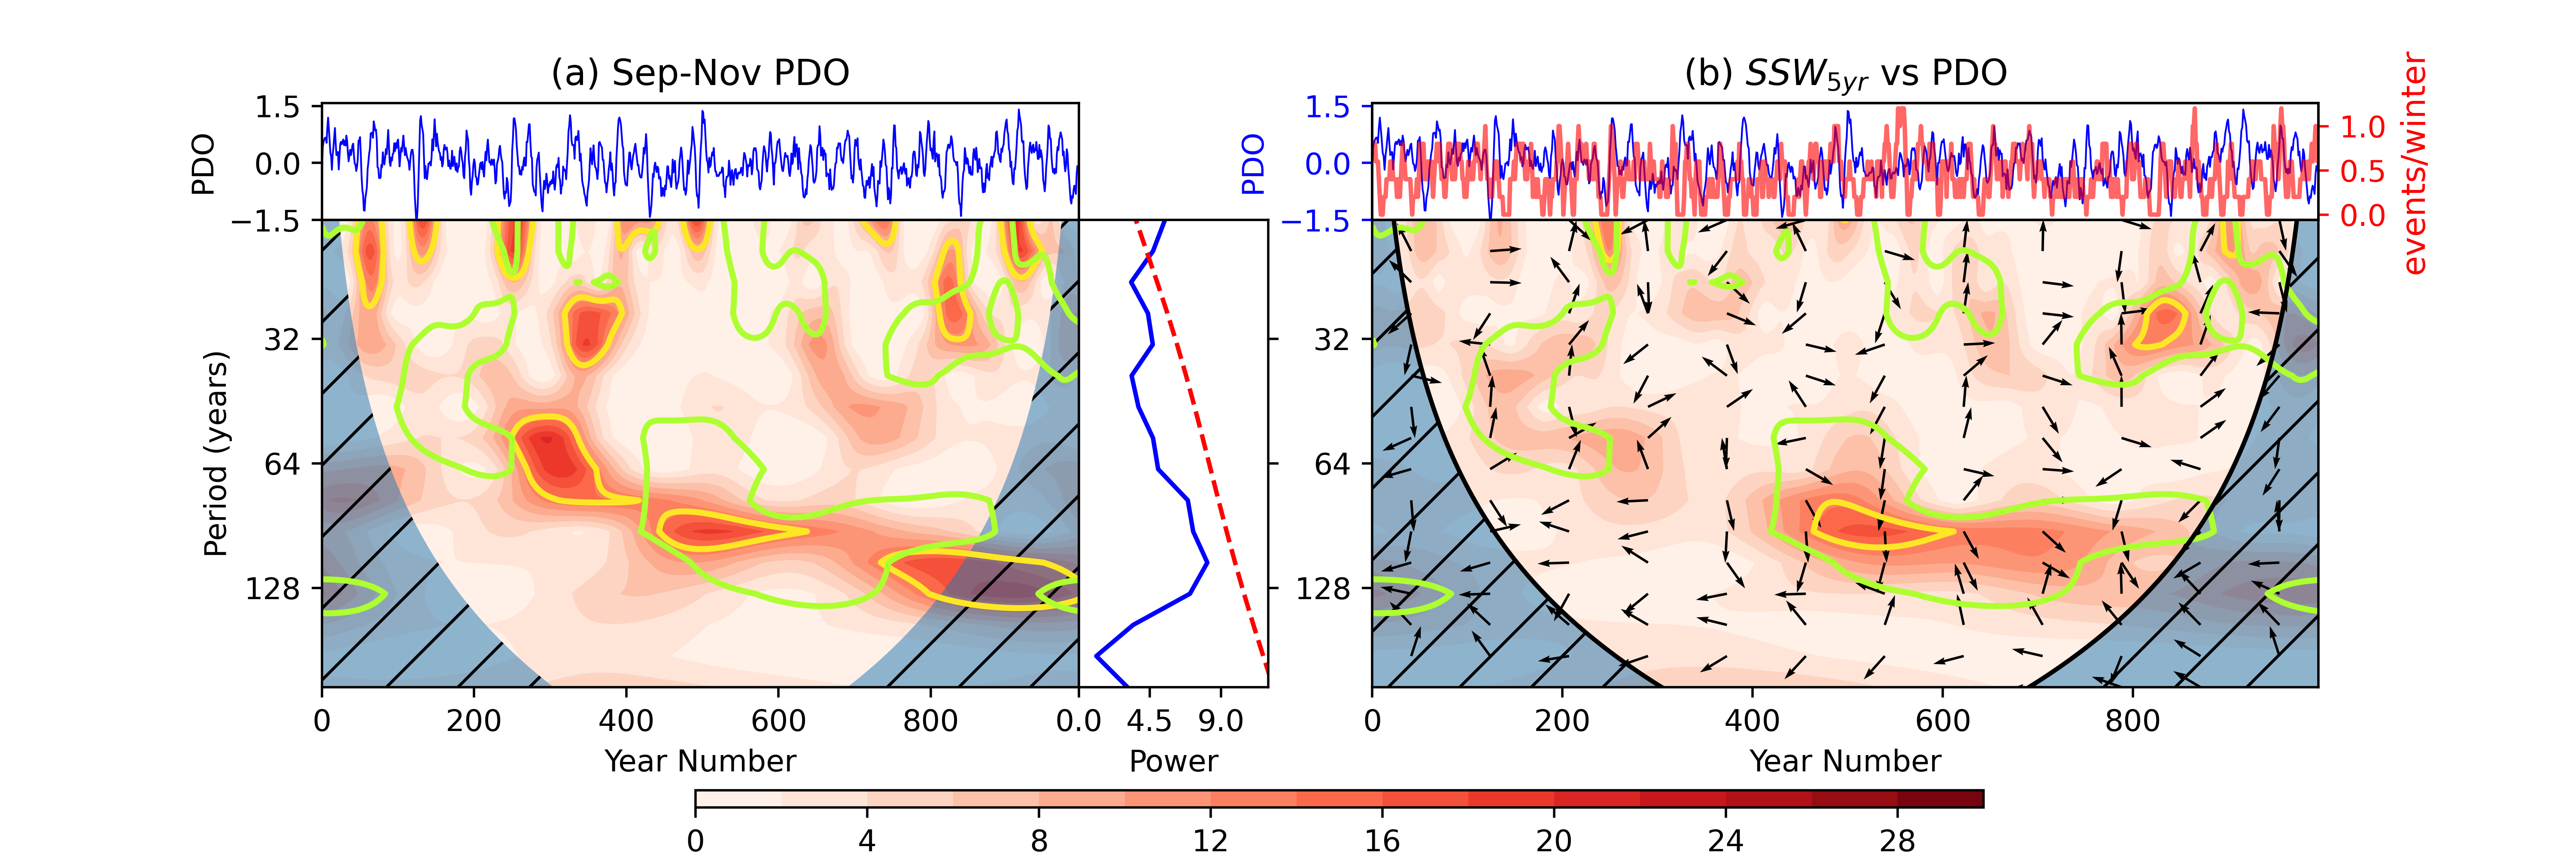
\includegraphics[width = \linewidth]{new_changed_figures/PDO_wavelet_combined_new_levels.png}
\caption{\textbf{(a, top)}: Sep-Nov PDO time series, \textbf{a, bottom left}: Wavelet power spectrum (shaded contours represent wavelet power and yellow contours the 95\% significance level compared to an AR1 process), \textbf{a, bottom right}: global wavelet power spectrum (blue) and 95\% confidence level (dashed red). \textbf{b}: Cross spectra between $SSW_5yr$ and the PDO index. \textbf{b, top}: PDO and $SSW_5yr$ time series. \textbf{b, bottom}: Cross power spectrum. Shading indicates cross power, yellow contours the 95\% confidence interval and arrows the relative phase angle between signals in the time series. Green contours on both spectra represent the 95\% confidence intervals for the wavelet power spectrum of $SSW_{5yr}$.}
\end{figure}
\end{center}


\begin{center}
\begin{figure}[h!]
\noindent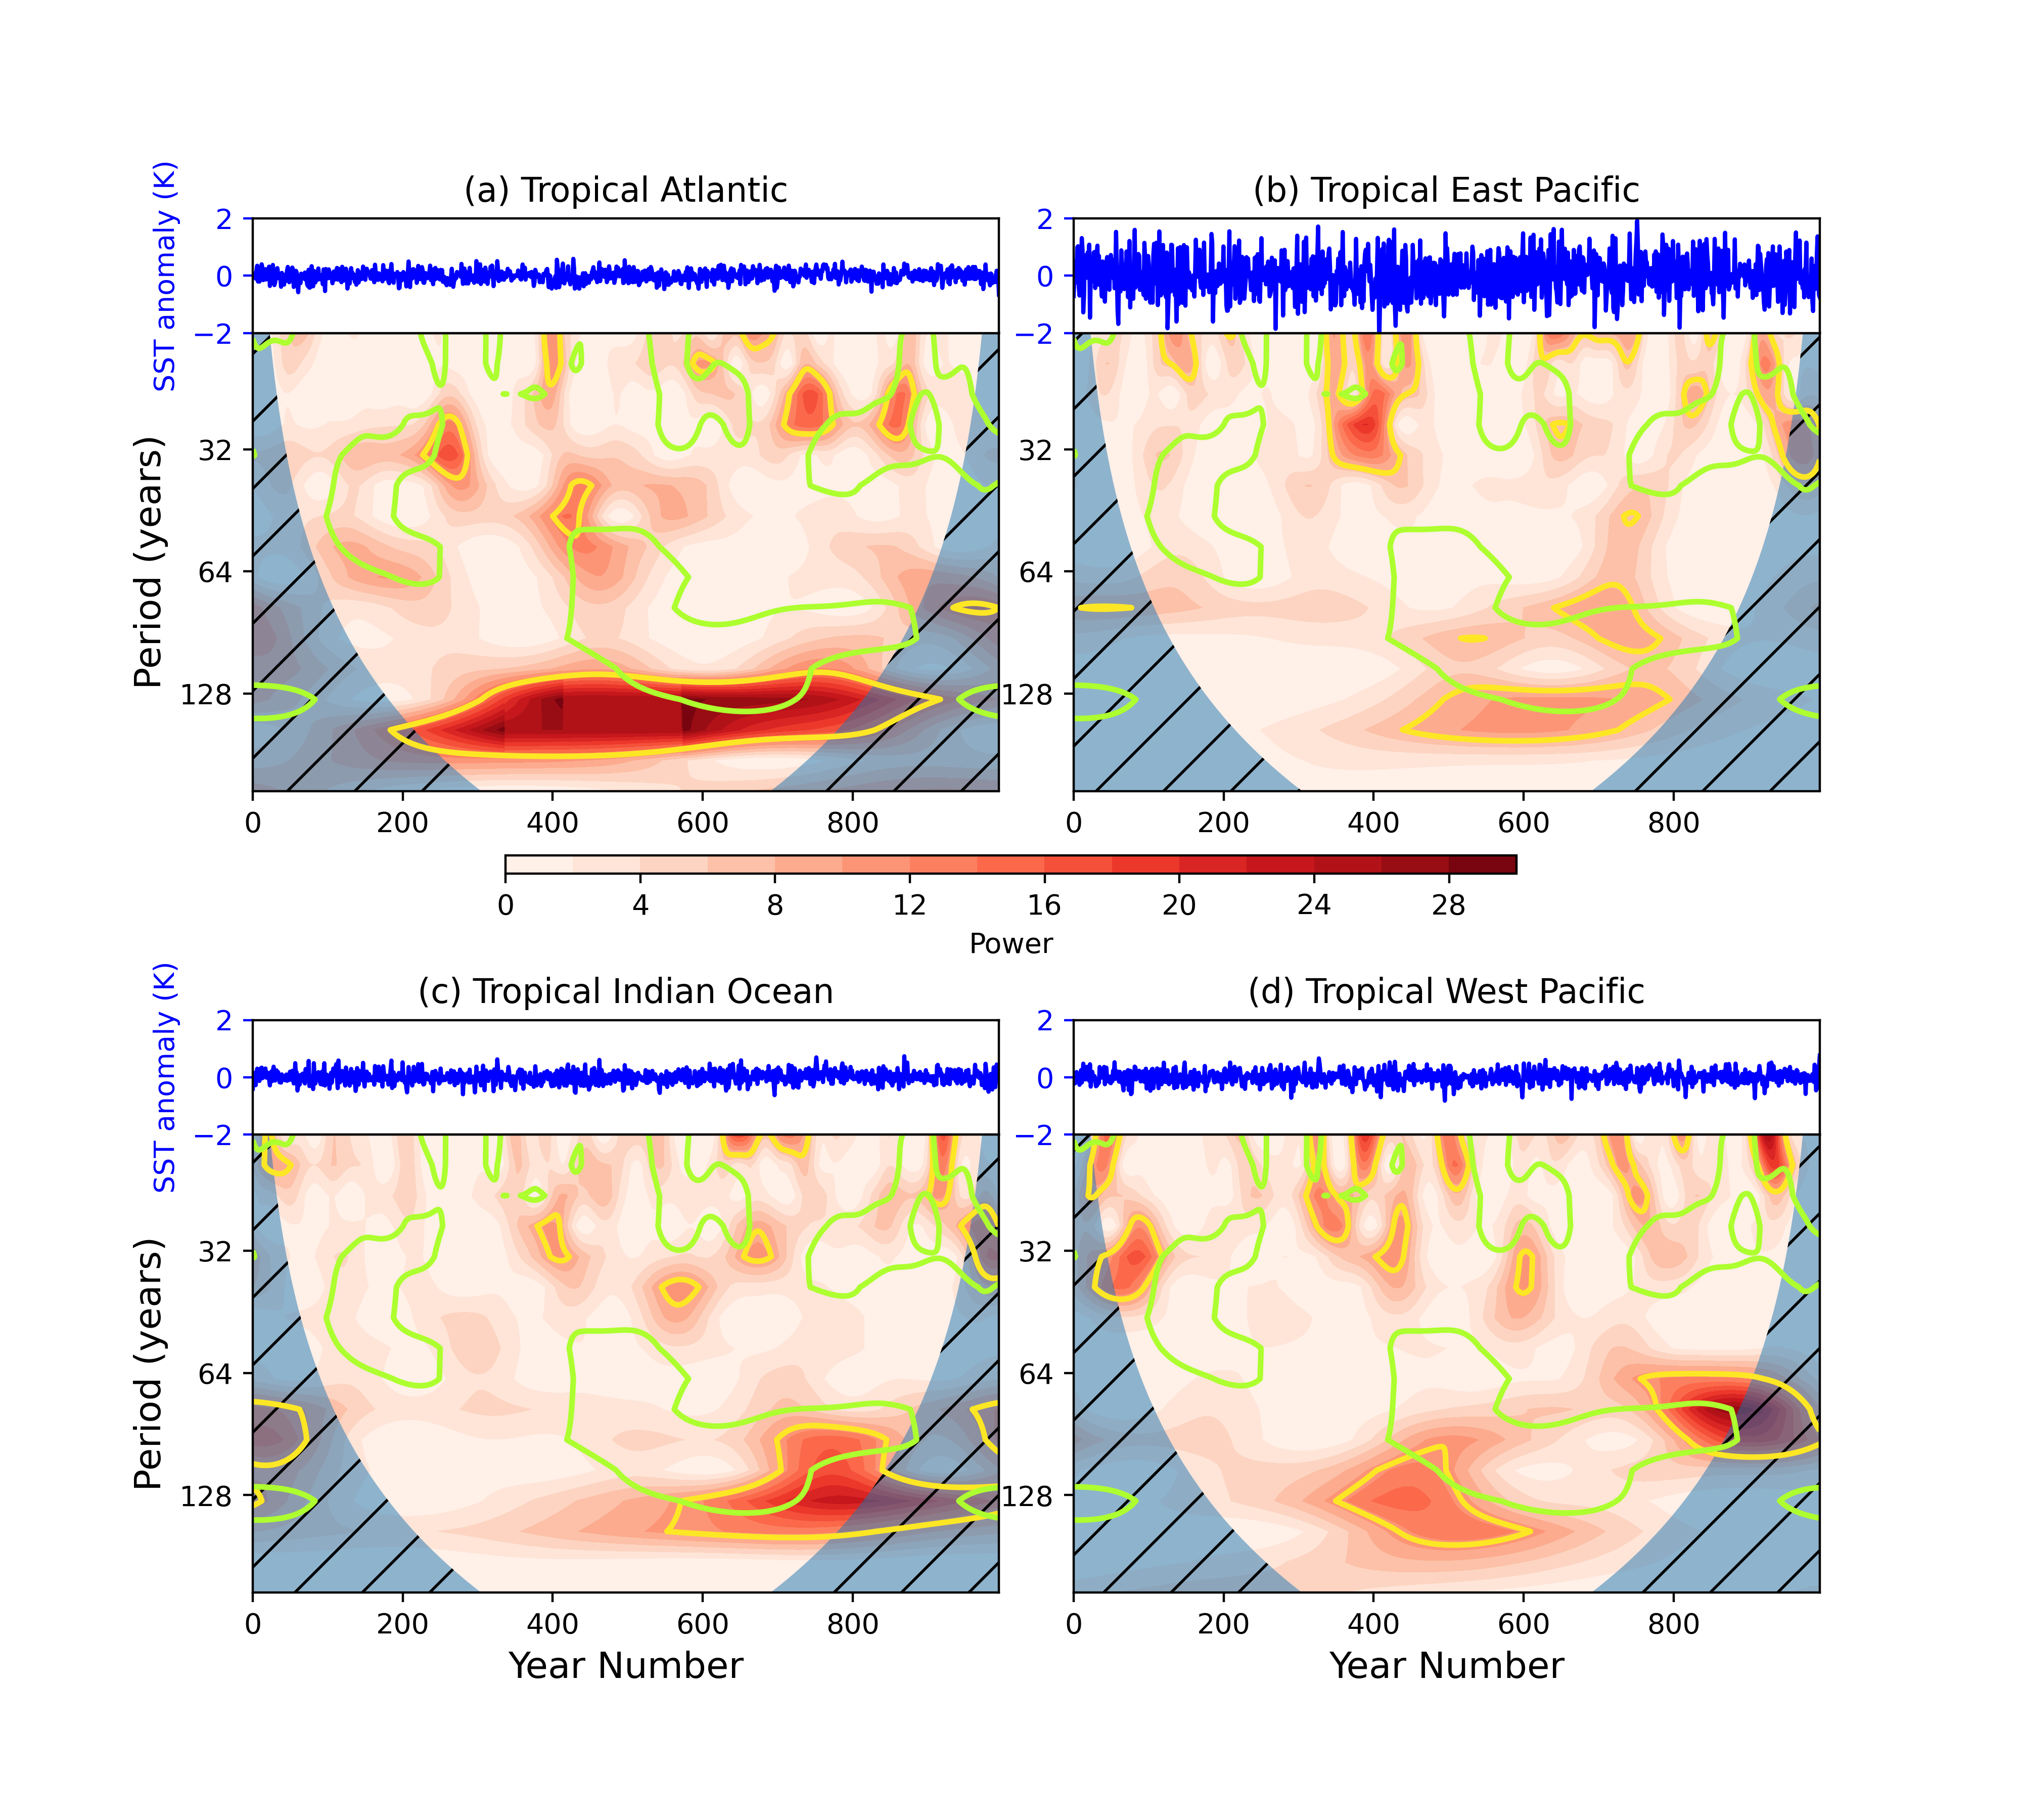
\includegraphics[width = \linewidth]{new_changed_figures/SSTs_tropical_wavelet_new_levels.png}
\caption{Sep-Nov SST anomaly time series and associated wavelet power spectrum for Tropical Atlantic (5$^{\circ}$\,S–5$^{\circ}$\,N, 60$^{\circ}$\,W–0$^{\circ}$\,W), Tropical East Pacific (5$^{\circ}$\,S–1$^{\circ}$\,N, 160$^{\circ}$\,E–270$^{\circ}$\,E), Tropical West Pacific (5$^{\circ}$\,S–25$^{\circ}$\,N, 110$^{\circ}$\,E–140$^{\circ}$\,E) and Tropical Indian Ocean (5$^{\circ}$\,S–10$^{\circ}$\,N, 45$^{\circ}$\,E–100$^{\circ}$\,E). Shading indicates wavelet power, yellow contours show the 95\% confidence level when the power is compared to and AR1 red-noise process and green contours indicate the 95\% confidence level for the power spectrum of $SSW_5yr$.}
\label{fig3}
\end{figure}
\end{center}

\begin{center}
\begin{figure}[h!]
\noindent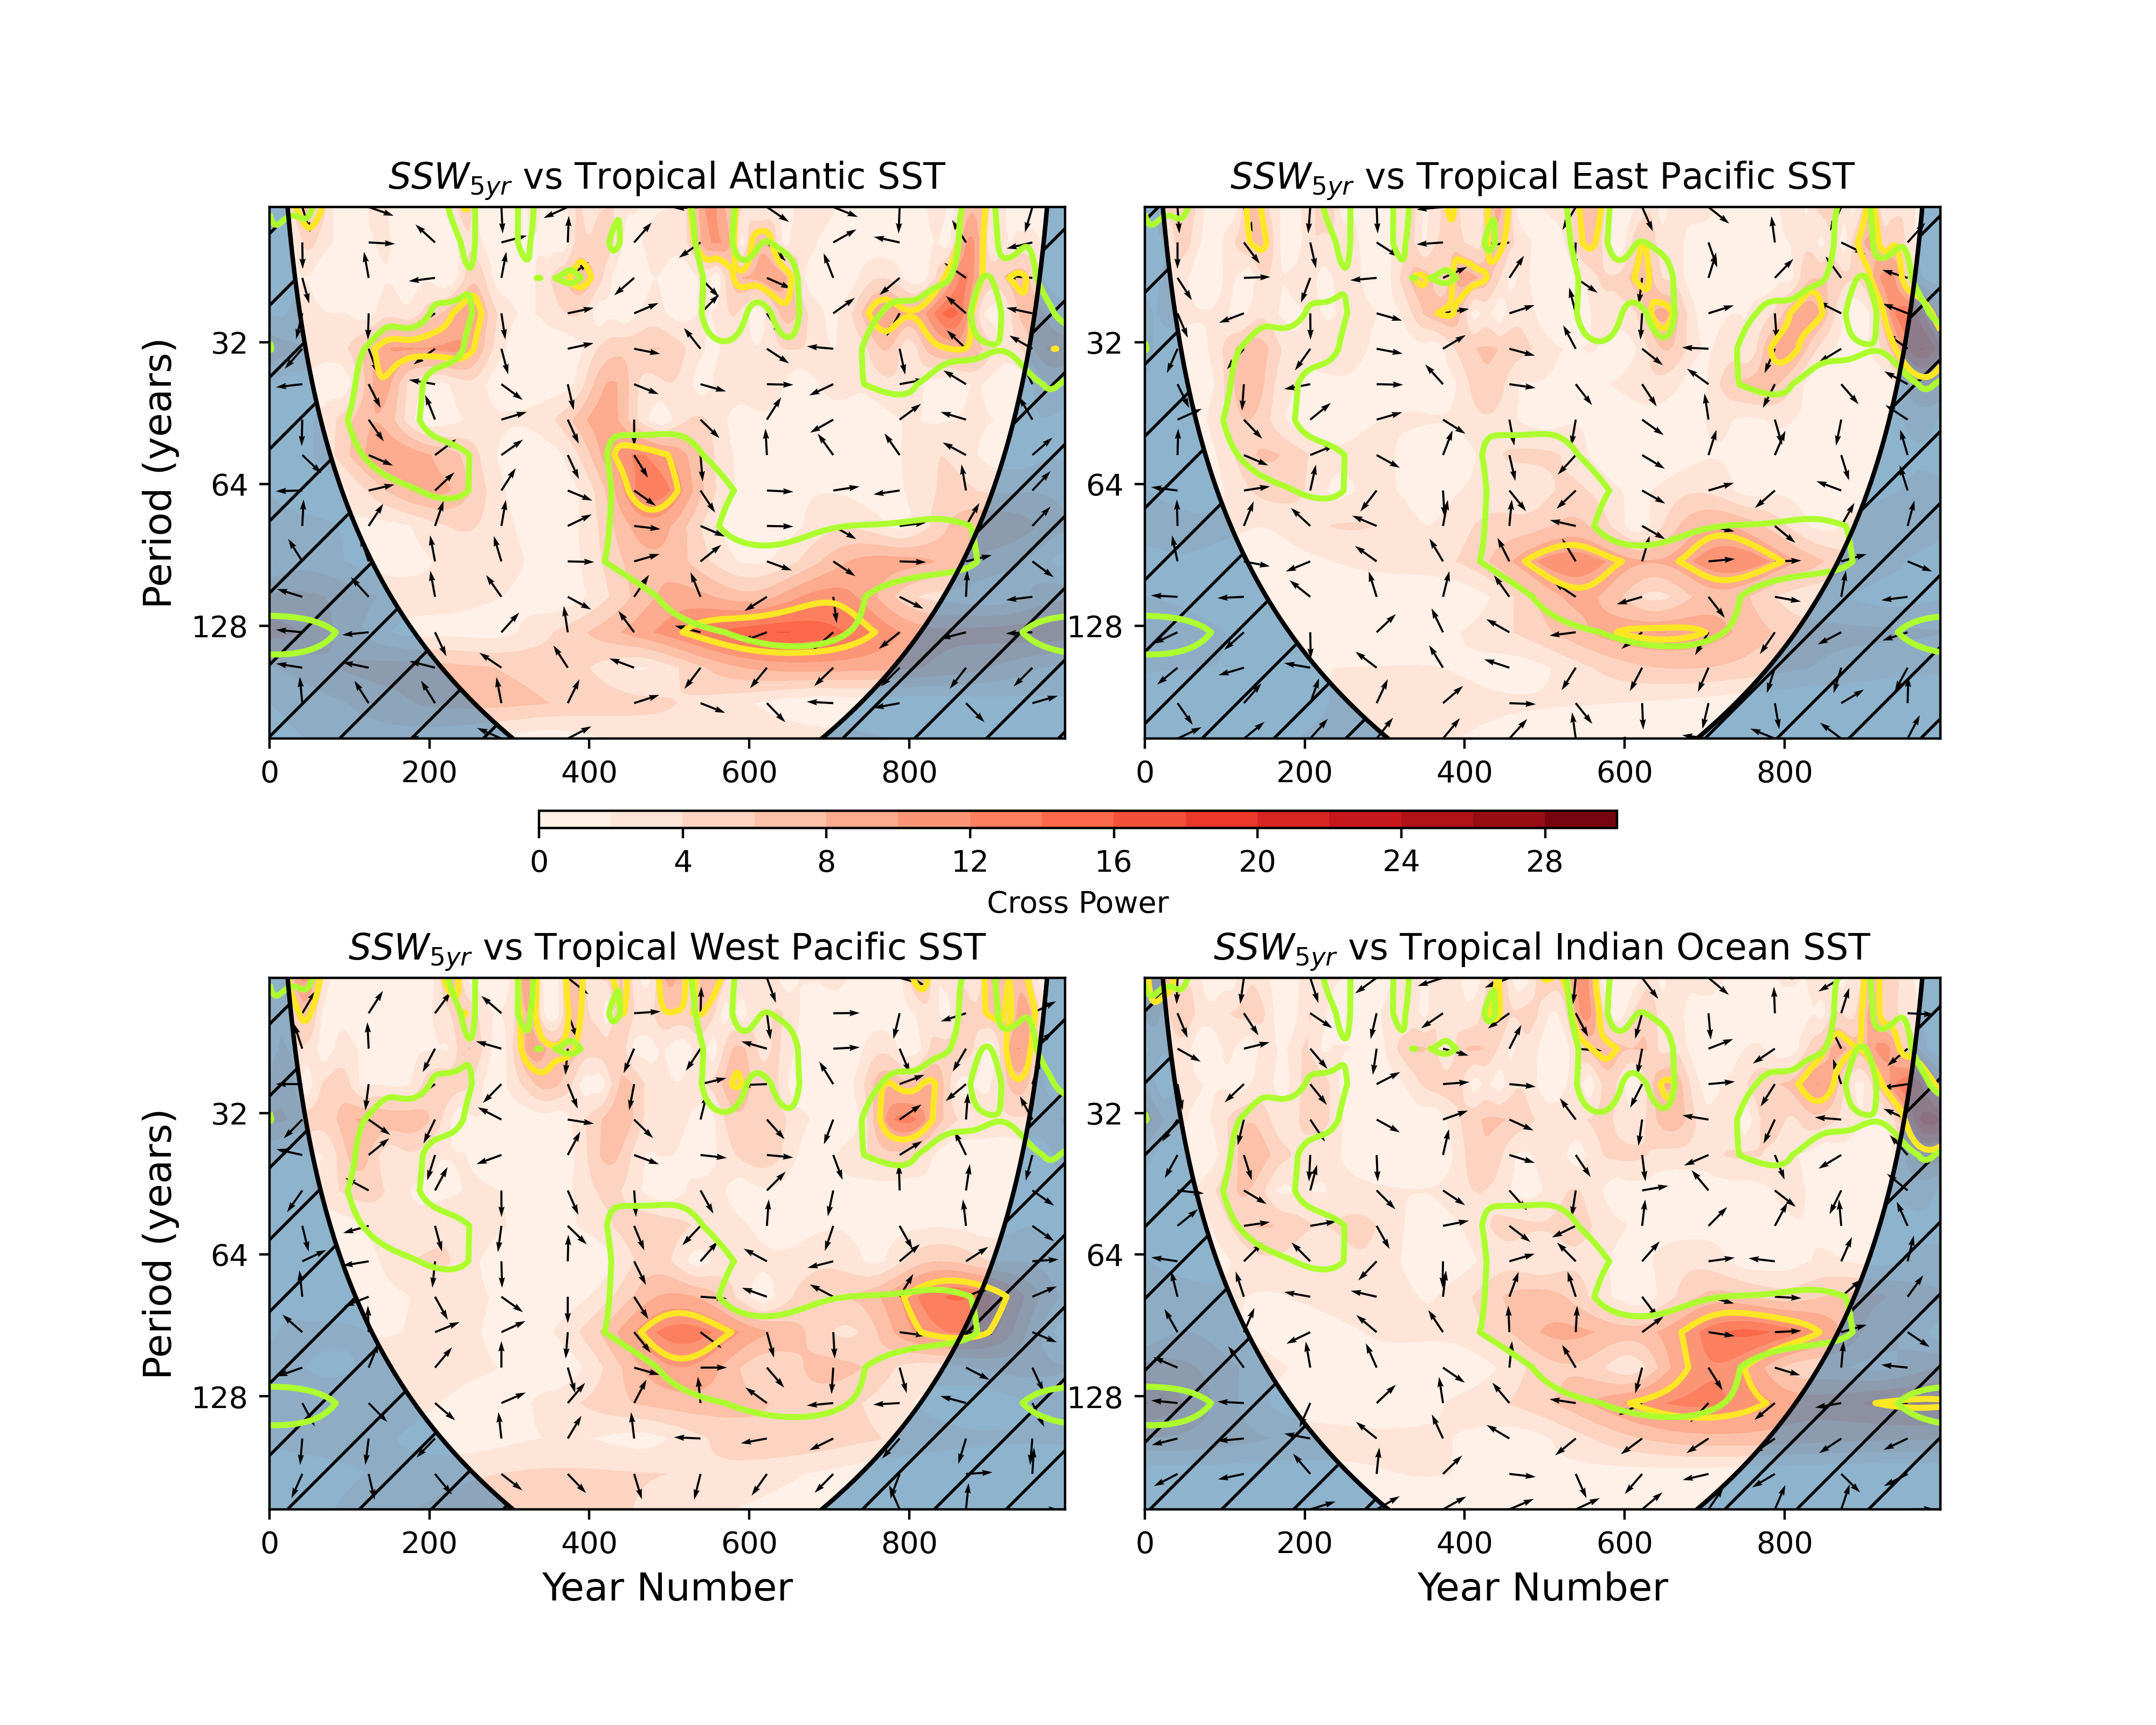
\includegraphics[width = \linewidth]{new_changed_figures/SSW_5yr_vs_trop_SSTs_crosspower_new_levels.png}
\caption{Cross power spectra between Sep-Nov Tropical SST anomaly time series and $SSW_5yr$. SST regions are defined as: Tropical Atlantic (5$^{\circ}$\,S-5$^{\circ}$\,N, 60$^{\circ}$\,W-0$^{\circ}$\,W), Tropical East Pacific (5$^{\circ}$\,S–1${^\circ}$\,N, 160$^{\circ}$\,E–270$^{\circ}$\,E), Tropical West Pacific (5$^{\circ}$\,S–25$^{\circ}$\,N, 110$^{\circ}$\,E–140$^{\circ}$\,E) and Tropical Indian Ocean (5$^{\circ}$\,S–10$^{\circ}$\,N, 45$^{\circ}$\,E–100$^{\circ}$\,E).}
\label{fig3}
\end{figure}
\end{center}


\begin{center}
\begin{figure}[h!]
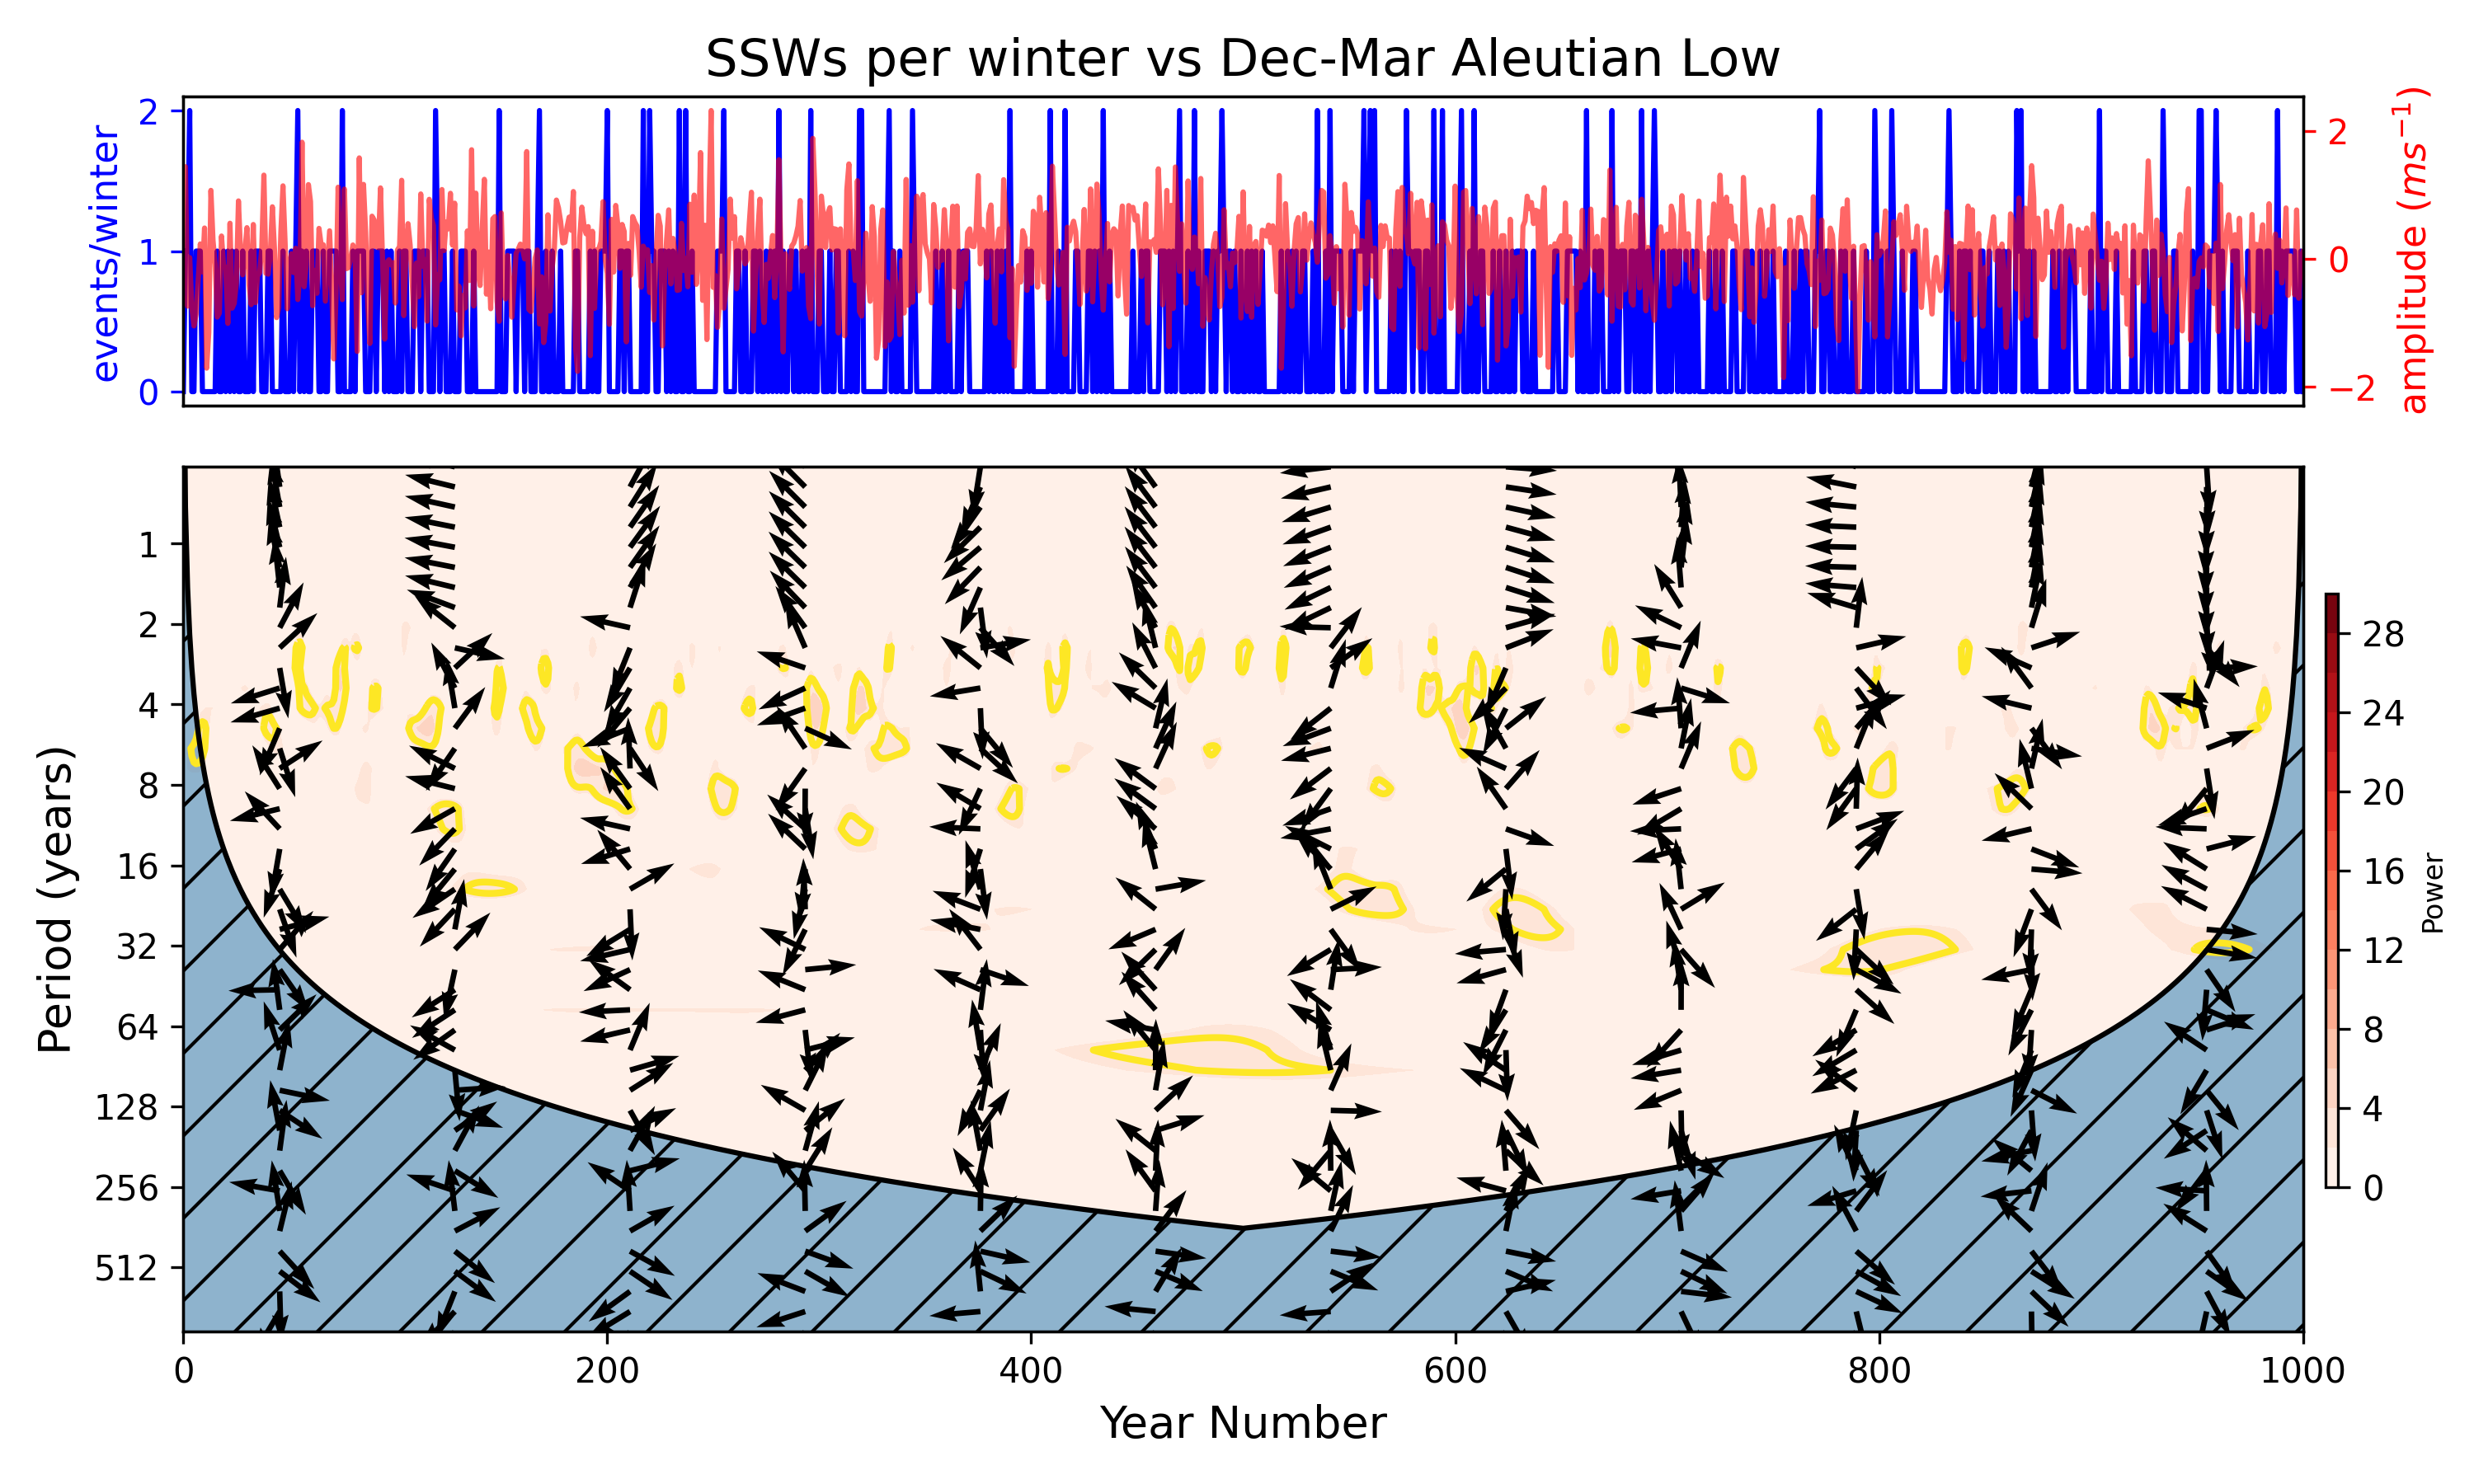
\includegraphics[width = \linewidth]{new_changed_figures/cross_power_SSWs_vs_AL_new_levels.png}
\caption{\textbf{Top}: Dec-Mar Aleutian Low index (red) and SSWs per NH winter (blue) time series. \textbf{Bottom}: Cross wavelet power spectrum between the two time series.}
\end{figure}
\end{center}

\begin{center}
\begin{figure}[h!]
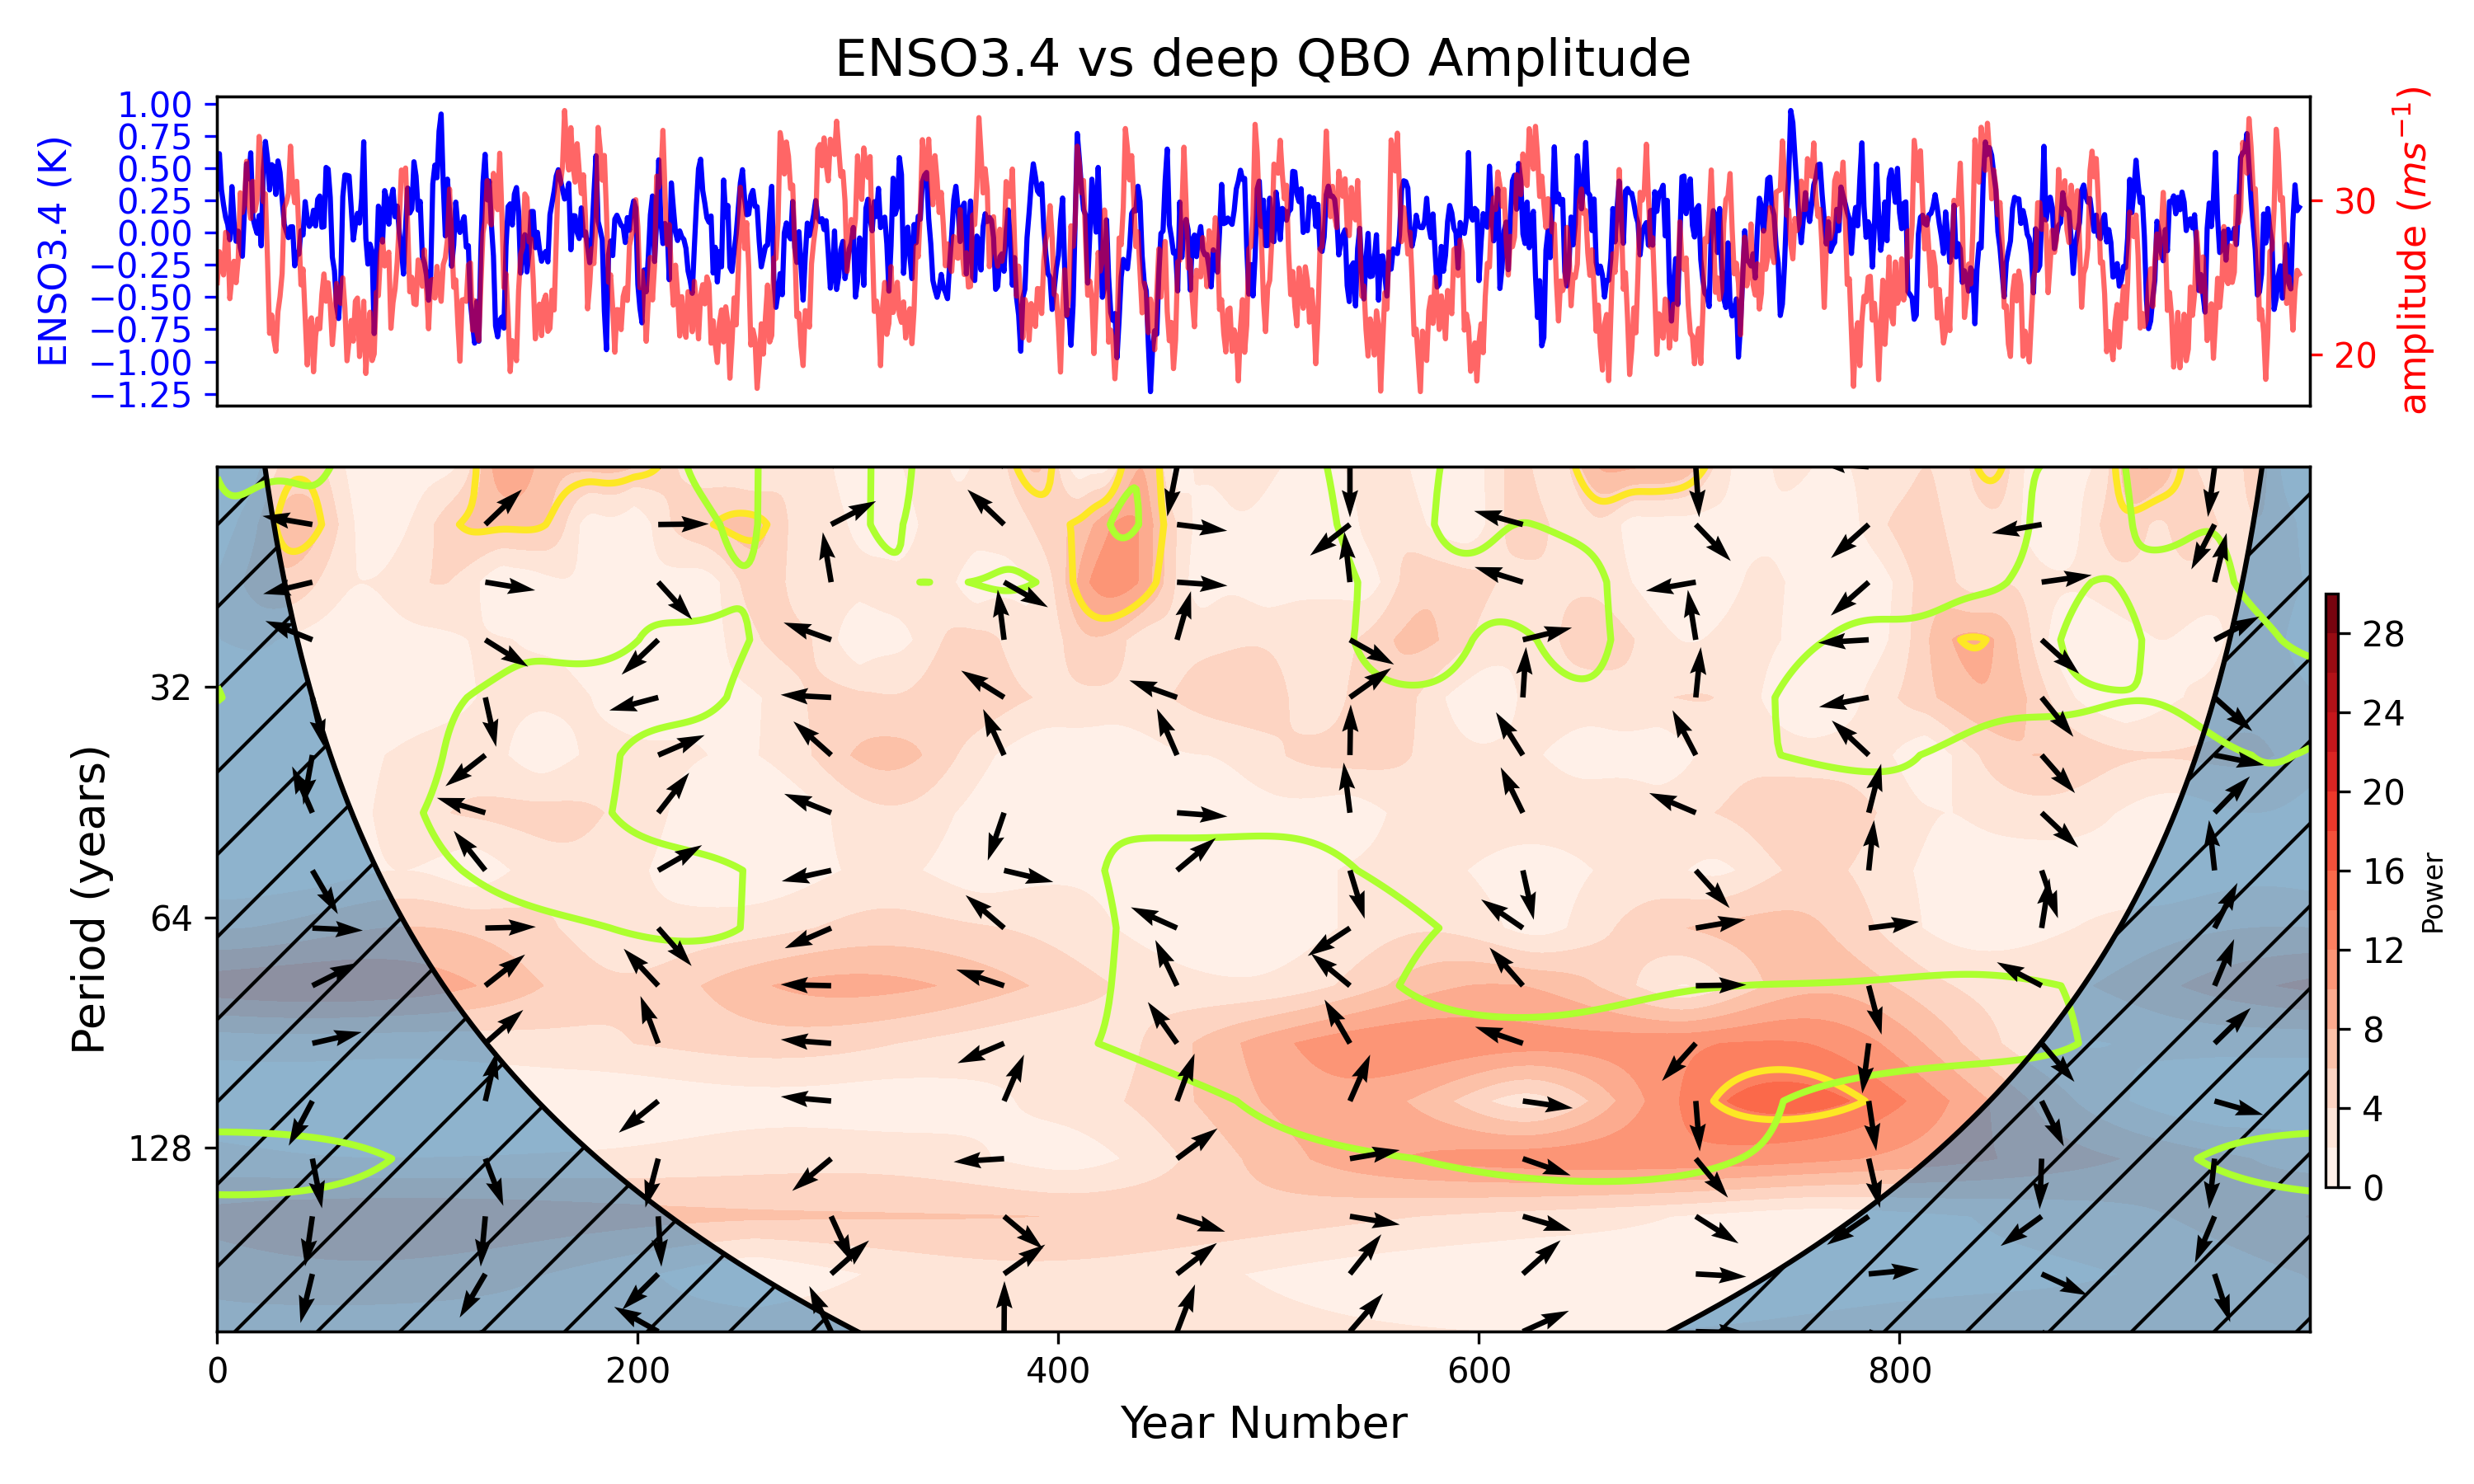
\includegraphics[width = 0.8\linewidth]{new_changed_figures/cross_power_ENSO_vs_deep_QBO_amp_5yr_mean_new_levels.png}
\caption{\textbf{Top}: Sep-Nov ENSO3.4 index  mean (blue) and Sep-Nov deep QBO Hilbert Amplitude index smoothed with a 5 year window (red). \textbf{Bottom}: Cross wavelet power spectrum between the two time series.}
\label{fig1}
\end{figure}
\end{center}

\begin{center}
\begin{figure}[h!]
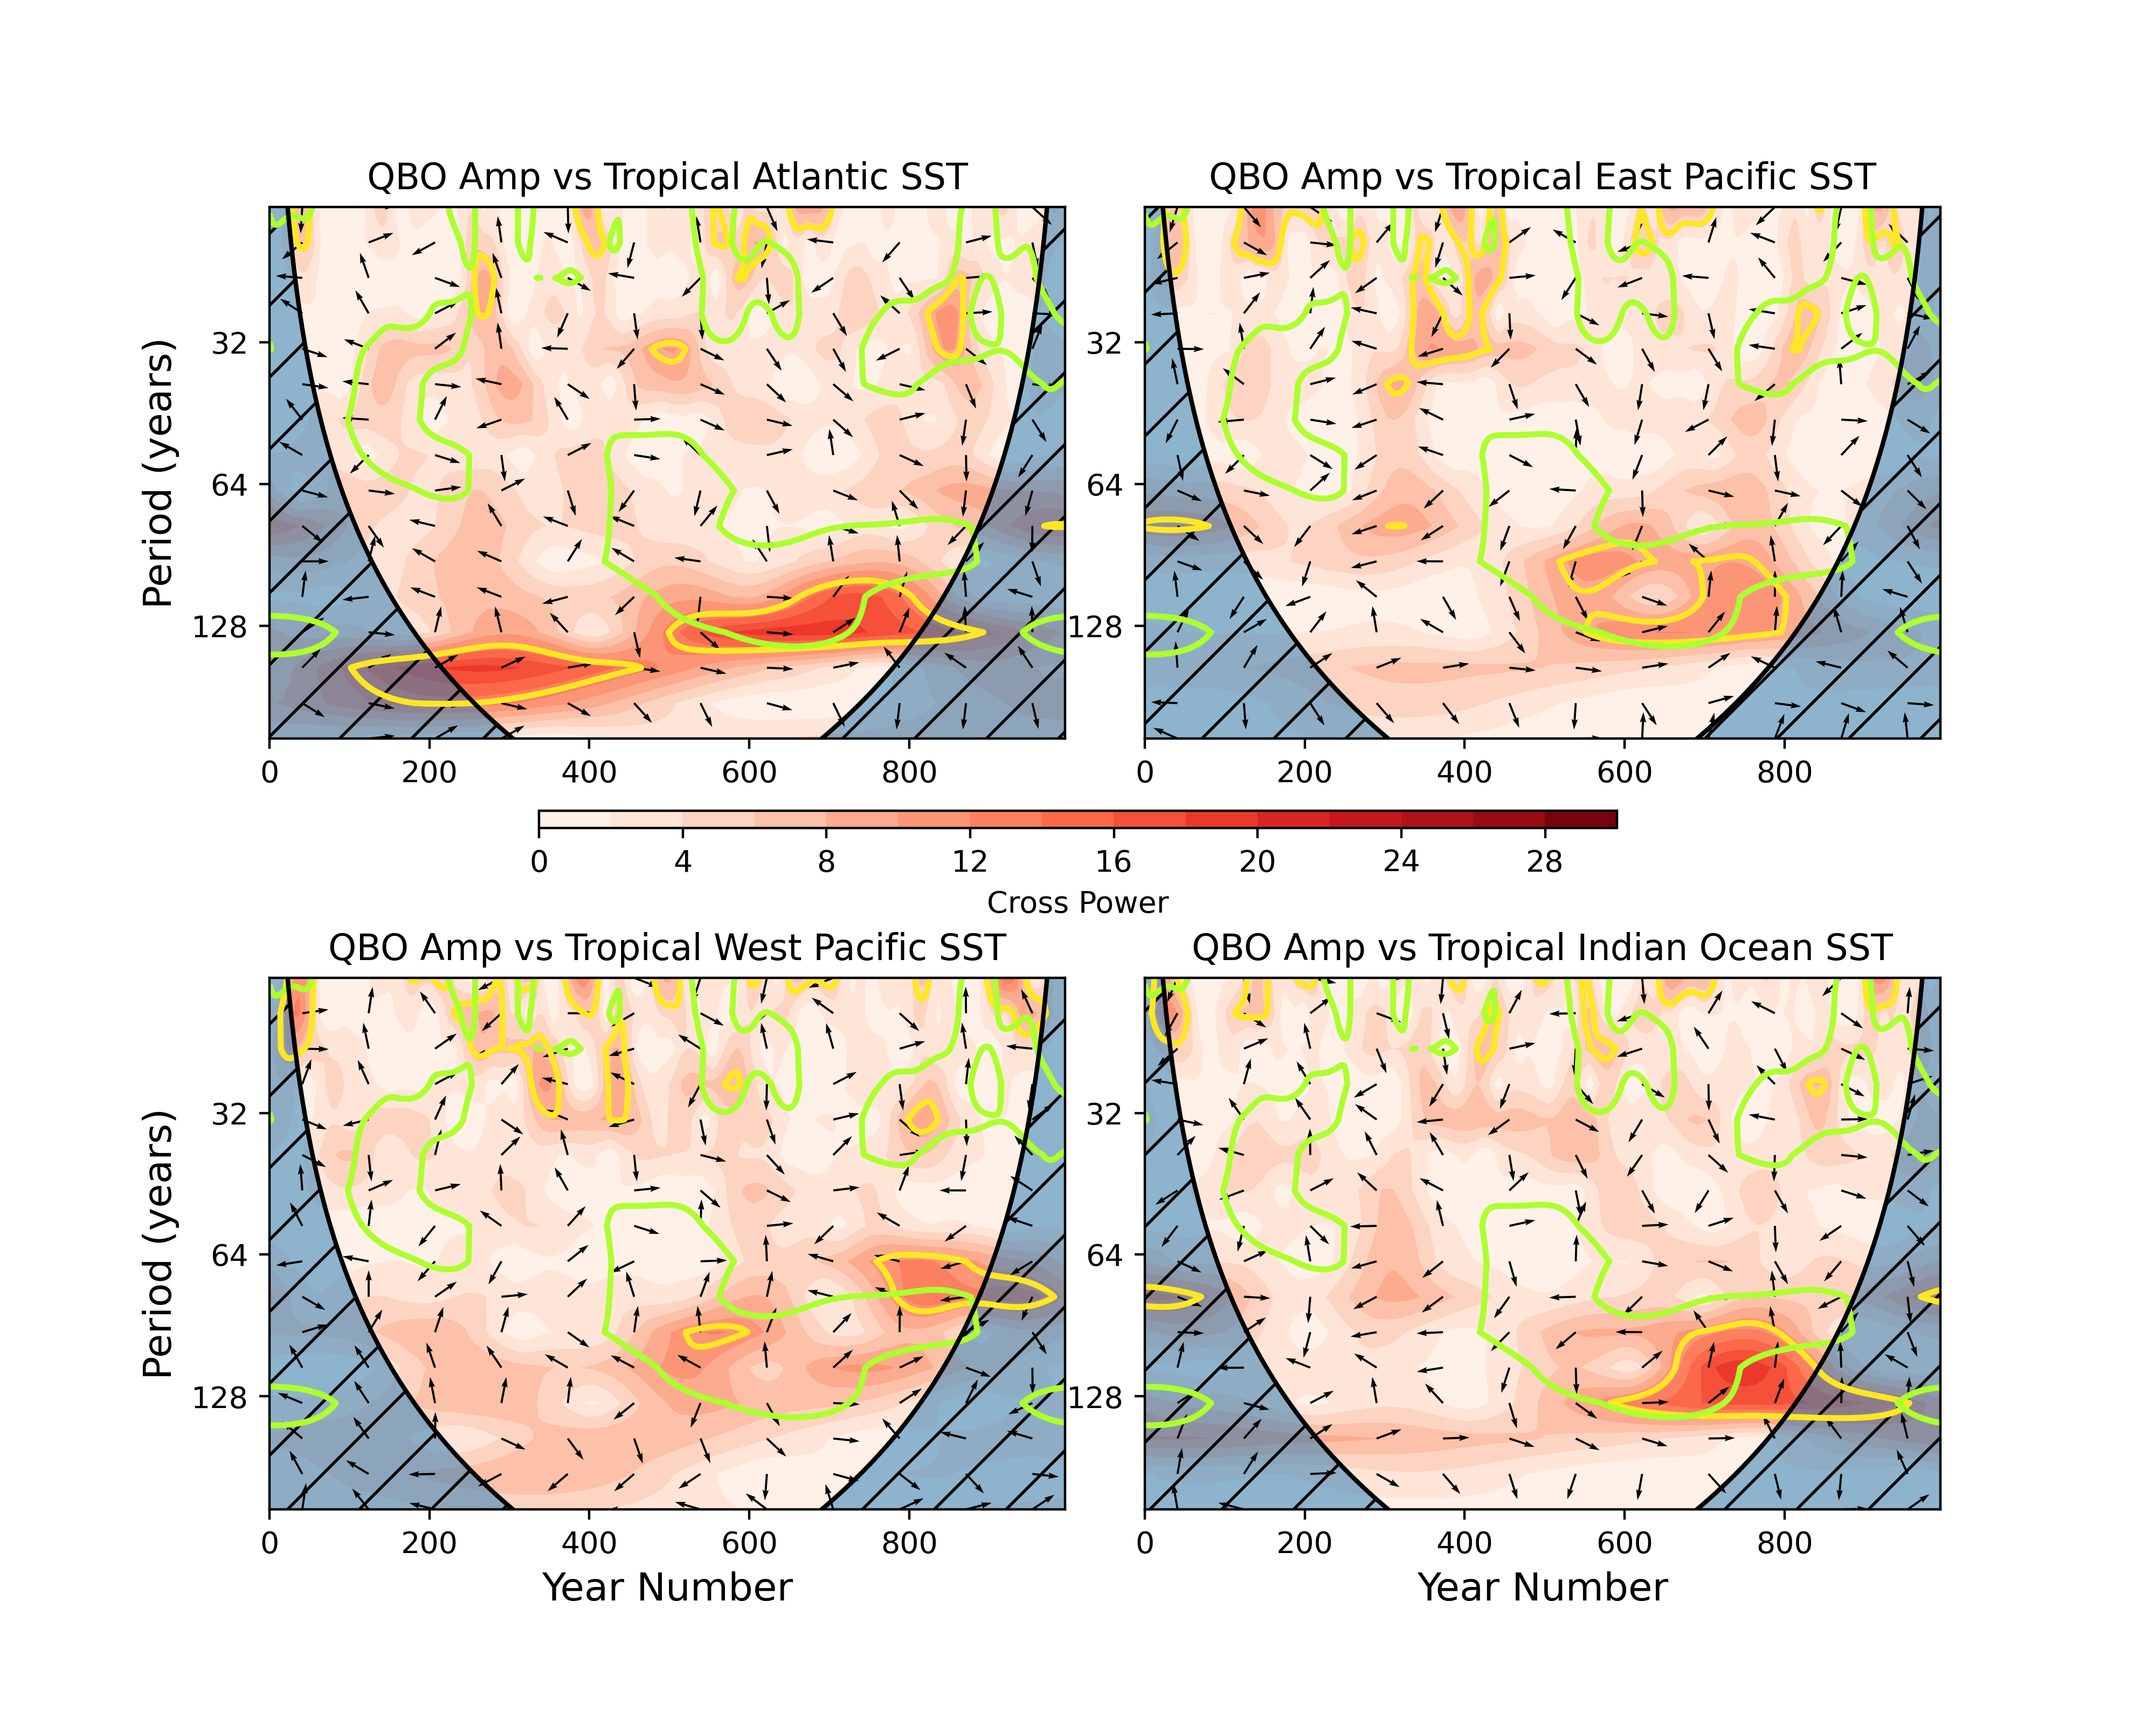
\includegraphics[width = \linewidth]{new_changed_figures/QBO_amp_vs_trop_SSTs_crosspower_new_levels.png}
\caption{Cross wavelet power spectra between Sep-Nov deep QBO amplitude modulation and Sep-Nov SST anomaly in each Tropical basin.}
\label{fig1}
\end{figure}
\end{center}


\end{document}


Unchanged text from here: ....... 

There are a number of supporting results for this hypothesis. First, we are able to show that the deep QBO metric which we consider in our spectral analysis exhibits strong coupling with the vortex when considering ZMZW composites (figure 3). This suggests coherent signals in QBO and SSW series may lead to a causal connection through a HT like relationship such as that studied in \cite{Gray2018}. Second, the multi-decadal signals in the deep QBO we find in the UKESM simulation is supported somewhat by previous works based on reanalysis which show that measures of QBO vertical coherence vary on such timescales \citep{Anstey2008, Yang2016}. Novel elements to our hypothesis such as the consideration of deep QBO amplitude modulation as the driver of SSW variability are not corroborated by previous work and will therefore require further study (outlined below). The Aleutian low has been shown in previous work \citep{Woo2015} to modulate planetary wave propagation into the stratosphere which is consistent with a possible link between signals in the AL metric and $SSW_{5yr}$ found here. However, coherence in these signals, while accounting for some power in $SSW_{5yr}$'s spectra, are far less persistent than those with the QBO. as a result, we refrain from making definitive statements regarding the AL-SSW link but recommend connections on this timescale be studied further. 

Despite the novel and potentially important results presented here, our analysis has a number of limitations which we intend to address in a body of further work. First, while we have identified statistically coherent signals in the QBO and SSWs, this does not confirm causal connections between them. A possible natural approach to determining connections could be to apply multi-linear regression techniques to the SSW and QBO time series while also incorporating the surface metrics mentioned above to evaluate the portion of $SSW_{5yr}$ variance accounted for by other variables. We expect however, that this method may suffer from a number of pitfalls, namely the non-stationary nature of signals we are considering as well as the potential non-orthogonality of explanatory variables (ENSO, QBO, AL). Instead of using such methods, we propose to test the robustness of our result by designing a set of sensitivity experiments in which QBO variability is fixed. These experiments will take the form of a set of GCM simulations in which the amplitude of the deep QBO is either allowed to evolve freely (as is the case in the PI control) or is nudged towards a constant value (i.e. with no amplitude variation). Comparison of multi-decadal signals in SSWs from these runs could confirm the key causal link between deep QBO amplitude and the vortex which is suggested by results in this study. Second, our result is derived from a single simulation of a single GCM - UKESM. The model exhibits biases in its mean SSW rate, which we attempt to allow for by only considering Dec-Mar SSWs, as well as a lengthened period of the QBO compared to ERA-Interim \citep{Bushell2020}. This could lead to an over-inflated HT strength due to longer persistence of QBO phases altering the mid-latitude waveguide through NH winter. As a result, teleconnections found in UKESM may not be fully representative of the real atmosphere. Recent work has also shown a large degree of inter-model variability exists in representations of the QBO as well as SSWs \citep{Bushell2020,ayarzag2020} so it is possible the result from this study is model dependant. Further work could consider a set of CMIP6 models and examine the signals in QBO and SSW time series. 

Open questions also remain regarding the role of signals in SSW time series in the earth system. If, as we propose here, amplitude modulation in a deep QBO metric is responsible for driving SSW signals, a natural area of further research could focus on understanding the cause of such amplitude variability. Categorising whether QBO signals are externally driven by features such as tropical upwelling, ENSO (as well as other tropical SST variability) and deep convection or internally generated would likely be key for this understanding. Cross power between QBO amplitude and ENSO3.4 index (supp figure A8) shows few significant signals with little coincidence in time-period space with SSW signals. The same is apparent for signals in QBO amplitude and other SST basins (supp figure A9). The true role of SST-QBO interactions in SSW variability may be determined with sensitivity runs similar to those outlined above but with prescribed SST patterns. Comparison of QBO features in prescribed and coupled SST simulations may indicate origins of QBO variability. 

Furthermore, while we suggest a set of drivers for periodic signals in SSWs, we do not assess the influence of hiatuses on the surface and particularly the NH Ocean basins which may be significant given the timescale of variability considered in this study. Further work could examine the interaction between signals in SSW time series and key modes of Atlantic and Pacific variability such as SSTs (the Atlantic Multi-decadal Variability index and Pacific Decadal Oscillation), circulation (the Atlantic Meridional Overturning Circulation index) as well as sea ice coverage. 

despite the possible shortcomings of this analysis, findings may point to a novel source of understanding and predictability in SSW emergence. This in turn could impact decadal predictability of NH winter surface climate (given SSWs' role in stratosphere-troposphere coupling), an area in which significant improvement can be made on current capabilities \citep{Zhang2019}. This work also suggests the possible importance of a new QBO metric, the deep QBO amplitude modulation, which couples with vortex variability. This points towards the need to include such metrics in future work analysing HT mechanisms in observations and model data. \textbf{(I am not sure about this final paragraph, seems a little weak at the moment)}
